\documentclass [4pt,a4paper,oneside,openany]{book} %Classe del documento, formato carta, singola facciata, apertura capitoli pag destra/sinista (ininfluente se impostato oneside). Formato libro
\usepackage{lmodern}
\usepackage[T1]{fontenc}
\usepackage[utf8]{inputenc}
\usepackage{cite}
\usepackage[italian]{babel} %Lingua Documento (da impostare per la sillabazione)
\usepackage{graphicx} %Pacchetto necessario per la gestione delle immagini
\usepackage{listings} %Per inserire codice
\usepackage[usenames]{color} %Per permettere la colorazione dei caratteri
\usepackage{subfigure}
\usepackage{Pacchetti/algpseudocode} %Pacchetto per l'immissione di pseudocodice
\usepackage[boxed]{Pacchetti/algorithm} %Pacchetto per l'immissione di pseudocodice
\usepackage{amsmath} %Simboli matematici
\usepackage{amsfonts} %Simboli matematici
\usepackage{amssymb} %Simboli matematici
%%\usepackage{Pacchetti/mcode}  %Pacchetto per l'immissione di codice matlab
%%\lstloadlanguages{C}
\usepackage {fancyhdr} %Pacchetto per la gestione accurata della pagina
\usepackage {setspace} %Pacchetto necessario per i comandi successivi onehalfspacing, singlespacing....
\usepackage{longtable} %Pacchetto per la gestione delle tabelle grandi
\usepackage[colorlinks=true]{hyperref} %Segnalibri nel pdf finale, sotto relativi parametri
\hypersetup{
	bookmarksnumbered=true,
	linkcolor=black,
	citecolor=black,
	urlcolor=black,
}
\lstset{
	language=C,
	basicstyle=\small\ttfamily,
	keywordstyle=\color{green}\bfseries,
	commentstyle=\color{red},
	stringstyle=\color{blue},
	showstringspaces=false
}
\usepackage{geometry} % Dimensione pagina
\geometry{a4paper} % Formato carta
\addtolength{\textheight}{75pt} %Margini
\oddsidemargin 30pt

\begin{document} %Inizio Documento

%%FRONTESPIZIO%%=========================================
\begin{titlepage}
 \begin{center}
     
\includegraphics[width=6cm]{Immagini/logo.png}\\ %Logo dell'Università, cambiare il percorso, se necessario
     \vspace{1em}
     {\Large \textsc{Universit\`a degli studi di Perugia}}\\
     \vspace{1em}
     {\Large \textsc{Facolt\`a di Ingegneria}}\\
     \vspace{5em}
     {\LARGE \textbf{Appunti di Sicurezza Informatica}}\\
 \end{center}
 
 \vskip 2.5cm
  \begin{center}
	\Large{\textit{Alessio Burani}}\\
	\Large{\textit{Silvia Cascianelli}}\\[0.4cm]
  \end{center}

\vskip 2.5cm
\begin{center}
{\normalsize Anno Accademico 2014/2015}
\end{center}
\end{titlepage}


%%INTESTAZIONI PAGINA%%====================================
\pagestyle{fancy}
\renewcommand{\chaptermark} [1]{\chaptername\ \thechapter.\ #1}{} 
\renewcommand{\chaptermark}[1]{\markboth{\thechapter.\ #1}{}} 
\renewcommand{\sectionmark}[1]{\markright{\thesection\ #1}}
\fancyhf{}
\fancyhead[LE,RO]{\bfseries\thepage} 
\fancyhead[LO,RE]{\bfseries\leftmark} 
\fancypagestyle{plain}{%
\fancyhead{} % leva l'intestazione
\renewcommand{\headrulewidth}{0pt} % e la linea
}

%%INDICE%%==============================================
\tableofcontents


%%CAPITOLI===============================================
\chapter{Introduzione alla sicurezza informatica}


\section{Premessa}

\subsection{Definizione}
Che cosa significa sicuro? La parola sicurezza e l’aggettivo sicuro vengono sempre associati a beni che si desidera proteggere da possibili danni, danneggiamenti, perdita, e via dicendo. In particolare un bene è al sicuro se è ben protetto, e la sua messa in sicurezza non deve impedirne l'utilizzo. Esistono molteplici definizioni di sicurezza informatica, ad esempio:
\begin{itemize} 
  \item Security is the degree of protection against danger, damage, loss, and criminal activity ~\cite{wikiSecurity}.
  \item Security is a form of protection where a separation is created between the assets and the threat ~\cite{isecomSecurity}.
\end{itemize}
La parola sicurezza deriva dal latino sine cura: senza preoccupazione. La sicurezza di un sistema può essere definita come la conoscenza del fatto che l’evoluzione del sistema non produrrà stati indesiderati. Le cause che possono minare la sicurezza sono molteplici e spesso
non prevedibili, quindi non si può parlare di sicurezza in senso assoluto, ma solo relativo (\textit{"L'unico computer sicuro è un computer spento"}).

\textbf{Trasversalità della tematica:} Le problematiche di sicurezza interessano molteplici campi (attività lavorative, vita domestica, hobby, giochi, sport, etc.). Di fatto, ogni settore della vita moderna ha delle implicazioni relative alla sicurezza. Il livello di sicurezza di un'organizzazione dipende dai livelli di sicurezza di tutti i suoi comparti/settori. Il livello di sicurezza di un sistema è determinato dal livello di sicurezza dal suo comparto meno sicuro (principio dell'anello debole).


\section{Concetti fondamentali}

\subsection{Sistema informativo e informatico}
\begin{itemize} 
  \item Per sistema informativo (information system) di un’organizzazione si intende l’insieme delle informazioni prodotte ed elaborate e delle risorse umane, materiali e immateriali, coinvolte nel processo di elaborazione di tali informazioni
  \item Per sistema informatico (information and communication technology system) s'intende l'insieme delle varie tecnologie coinvolte nel sistema informativo (il sistema informativo è parte del sistema informatico).
\end{itemize}
Questo corso verterà sulla sicurezza dei sistemi informativi. Tuttavia, si approfondiranno maggiormente questioni inerenti la sicurezza
dei sistemi informatici. Per sicurezza di un sistema informativo si intende il grado di protezione contro qualsiasi minaccia ai suoi asset.
Richiede il soddisfacimento dei seguenti requisiti:
\begin{itemize} 
  \item \textbf{confidenzialità, integrità e disponibilità}
  \item \textbf{assicurazione, autenticità e anonimato}
\end{itemize}
Quando si parla di \textbf{attacco} solitamente si intende la violazione di uno o più di questi requisiti.

\subsection{Vulnerabilità, Minacce, Attacchi, Difesa}
\subsubsection{Vulnerabilità}
Una vulnerabilità (o falla o breccia) è una \textbf{debolezza intrinseca} di un sistema, che potrebbe essere sfruttata per provocare perdite o danni. Scaturisce spesso da errate procedure di sicurezza e/o da errori di progettazione/implementazione, e  in alcuni casi è intimamente legata alla natura del sistema. Ad esempio:
\begin{itemize} 
  \item un sistema potrebbe essere vulnerabile alla manipolazione non autorizzata dei dati causa un bug nella procedura di autenticazione dell’utente
  \item un calcolatore è vulnerabile all'acqua
\end{itemize}
Nel primo caso (vulnerabilità scaturite da errate procedure di sicurezza) l'insorgenza delle vulnerabilità può essere mitigata adottando adeguati standard e norme di qualità.

\subsubsection{Minacce (Threats)}
Per minaccia (threat) ad un sistema informatico/informativo si intende quell’insieme di circostanze che potrebbero arrecare danni ai suoi asset: eventi potenziali, accidentali o deliberati, che, nel caso accadessero, produrrebbero perdite e danni. il realizzarsi di una minaccia generalmente avviene sfruttando una o più vulnerabilità del sistema.  Si parla quindi di situazioni ipotetiche che potrebbero avvenire in determinate circostanze. Ad esempio:
\begin{itemize} 
  \item esecuzione di codice malevole che invia dati sensibili ad un'organizzazione criminale
  \item accesso a dati riservati da parte di entità non autorizzate
  \item perdita di dati a causa della rottura di un apparato hardware o al crash di uno specifico software
\end{itemize}

\subsubsection{Attacchi (Attacks)}
Un attacco (attack) è un atto deliberato teso ad arrecare un danno al sistema. Consiste, di fatto, nella realizzazione di una \textbf{minaccia}. Generalmente, un attacco viene perpetrato attraverso lo sfruttamento di una o più vulnerabilità. Spesso si classificano in base all’entità del danno:
\begin{itemize} 
  \item \textbf{attacco attivo (active attack)}: altera le risorse o ne modifica il processo di gestione/elaborazione
  \item \textbf{attacco passivo (passive attack)}: ottiene le informazioni/dati senza alterarli e senza modificare il relativo processo di
gestione/elaborazione
\end{itemize}
Un’altra importante classificazione è in base "al luogo" da cui viene iniziato l’attacco:
\begin{itemize} 
  \item \textbf{attacco dall’interno (inside attack)}: attacco iniziato da un'entità all’interno del perimetro di sicurezza di un sistema informativo di una data organizzazione
  \item \textbf{attacco dall’esterno (outside attack)}: attacco iniziato da un'entità all’esterno del perimetro di sicurezza
\end{itemize}
Ovviamente, è molto più difficile prevenire e rilevare gli attacchi interni di quelli esterni. Ciò anche a causa del fatto che le misure di prevenzione per questo tipo di attacchi limita notevolmente l'usabilità del sistema (si pensi, ad esempio, alla struttura gerachica in ambiente militare, in cui ogni risorsa conosce il minimo indispensabile per svolgere i propri compiti. In questo modo nel caso la risorsa venga compromessa, si limita il danno. Ovviamente tutto ciò rallenta il processo di funzionamento del sistema).

\subsubsection{Tecniche di difesa}
Diverse contromisure (o misure protettive) possono essere attuate per proteggere un sistema informativo da eventi accidentali e da
attacchi deliberati. Tali misure devono essere strutturate all’interno di un piano di sicurezza redatto dopo un’attenta analisi costi/benefici (textit{cost-effective solutions}).
Le tecniche di difesa possono essere di tipo:
\begin{itemize} 
  \item \textbf{preventivo}: effettuano una serie di \textbf{controlli} per evitare \textbf{a priori} che attacchi noti o immaginabili possano essere sferrati con successo (e.g. controlli aeroportuali, controllo di accessi e permessi negli OS).
  \item \textbf{a posteriori}: sono tese a ridurre gli effetti di un attacco che è riuscito a eludere le misure preventive di cui sopra; devono monitorare un sistema ed essere in grado di \textbf{rivelare} comportamenti anomali.
\end{itemize}

Un \textbf{meccanismo di sicurezza} è un qualsiasi metodo, strumento, o procedura teso a rilevare, prevenire o porre rimedio agli effetti di un attacco alla sicurezza del sistema. La strategia di difesa, qualunque essa sia, combina in modo opportuno
uno o più meccanismi di sicurezza. molti meccanismi di sicurezza consistono in controlli hardware/software.

\subsection{Sicurezza informatica: definizione classica e requisiti CIA}
La sicurezza informatica si fonda sulla protezione dei seguenti macro-requisiti di un sistema informativo (informatico):
\begin{itemize} 
  \item \textbf{Confidenzialità (Confidentiality)}
  \item \textbf{Integrità (Integrity)}
  \item \textbf{Disponibilità (Availability)}
\end{itemize}
Spesso si utilizza l’acronimo C.I.A. per denotarli in modo compatto.
\begin{figure}[htbp]
	\centering%
	\subfigure%
	{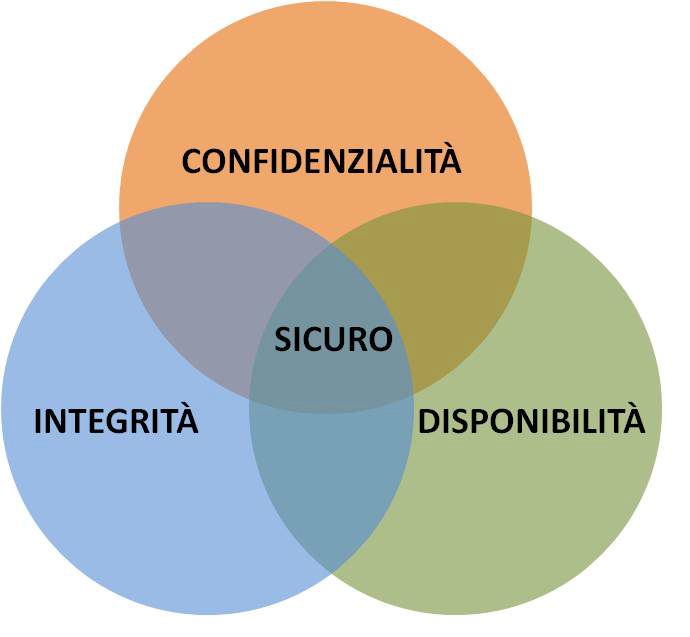
\includegraphics[height=7cm, width=7cm, keepaspectratio]{Immagini/Capitolo1/venn_security}}
	\caption{Diagramma di Venn dei macro-requisiti di sicurezza \label{fig:venn_security}} 	
\end{figure}
Ovviamente, come si può notare dal diagramma di Venn in \figurename ~\ref{fig:venn_security} spesso vengono richiesti contemporaneamente più di questi requisiti, cosi come un attacco può violare più requisiti.

\subsubsection{Confidenzialità (Confidentiality)}
Def. \textbf{Confidentiality}: the property that information is not made available or disclosed to unauthorized individuals, entities, or processes. Per confidenzialità si intende quindi la garanzia che alle risorse informatiche accedano solo le parti autorizzate ad accedervi. E' talvolta denominata segretezza, riservatezza o privacy. Nota bene: per accesso non si intende solo la lettura, ma anche la visualizzazione, la stampa o la semplice consapevolezza dell’esistenza di una data risorsa nel sistema.\newline

\textbf{Attacchi alla confidenzialità:} Si ha un attacco alla confidenzialità quando una entità (persona, processo o risorsa) tenta di accedere senza autorizzazione a informazioni protette (mentre queste sono memorizzate, oppure durante l’elaborazione, oppure ancora durante una comunicazione). La protezione della confidenzialità avviene utilizzando in modo appropriato i seguenti strumenti (meccanismi) di sicurezza informatica:
\begin{itemize} 
  \item \textbf{Cifratura (Encryption)}
  \item \textbf{Controllo degli accessi (Access Control)}
  \item \textbf{Sicurezza fisica (Physical security)}
\end{itemize}

\subsubsection{Integrità (Integrity)}
 Def. \textbf{Integrity}: safeguarding the accuracy and completeness of information and processing methods.\newline
 Def. \textbf{Integrity}: the property of safeguarding the accuracy and completeness of assets.\newline


Per integrità si intende quindi la garanzia che le risorse possano essere modificate solo dalle parti autorizzate e solo nei modi prestabiliti. Le modifiche comprendono la scrittura, la variazione, il cambiamento dello stato, l’eliminazione e la creazione. Nel caso di file, conviene includere anche i metadati associati (proprietario, ultimo utente ad averlo letto, data ultima modifica,data di creazione), in modo che un accesso non autorizzato al contenuto possa essere rivelato da un controllo di integrità applicato ai metadati.\newline

\textbf{Attacchi all'integrità:} Si ha un attacco all'integrità quando una entità (persona, processo o risorsa) tenta di modificare senza autorizzazione una o più risorse del sistema informativo.

 La protezione della confidenzialità avviene utilizzando in modo appropriato i seguenti strumenti (meccanismi) di sicurezza informatica (tutti basati su un uso corretto della ridondanza):
\begin{itemize} 
  \item \textbf{Backup}
  \item \textbf{Somma di controllo o Checksum}
  \item \textbf{Codici a correzione di errore (Corruzioni non deliberate ma accidentali, possono essere facilmente elusi da attacchi intelligenti)}
  \item \textbf{Codici di autenticazione dei messaggi o Message Authentication Code MAC} 
\end{itemize}


\subsubsection{Disponibilità (Availability)}
 Def. \textbf{Availability}: ensuring that authorized users have access to information and associated assets when required. \newline

Per disponibilità (availability) si intende quindi che le risorse siano accessibili, nei tempi e nei modi prestabiliti, alle parti autorizzate ogni volta che le richiedono: se una persona o un sistema dispone dei diritti di accesso ad una risorsa, l’accesso non deve essergli impedito. Spesso la disponibilità viene citata tramite il suo opposto: la \textbf{negazione di servizio} (\textbf{Denial of Service} o \textbf{DoS}). La disponibilità può assumere significati/sfumature diverse; una risorsa può trovarsi in uno stato intermedio tra i due opposti stati di piena disponibilità e di piena indisponibilità.

\subsection{Conflittualità requisiti CIA}

\subsection{Requisiti AAA}

\subsubsection{Assicurazione (Assurance)}

\subsubsection{Autenticità (Authenticity)}

\subsubsection{Anonimato (Anonymity)}

\subsection{Tipologie di Minacce e Attacchi}

\subsubsection{Intercettazione (Eavesdropping)}

\subsubsection{Alterazione (Alteration)}

\subsubsection{Interruzione (Denial-of-service)}

\subsubsection{Falsificazione (Masquerading)}

\subsubsection{Ripudio (Ripudiation)}

\subsubsection{Inferenza (Inference), Correlation and traceback}
Per inferenza o attacco inferenziale si intendono un insieme di tecniche che utilizzando la statistica e l’algebra permettono di ricavare/stimare \textbf{informazioni sensibili} a partire da dati non sensibili. Rappresenta un attacco alla confidenzialità, e spesso è attuato nel contesto dei databases. Similmente, per correlation and traceback si intendono un insieme di tecniche basate sulla statistica e sull’algebra che permettono di determinare la sorgente di una particolare informazione o di un particolare flusso di dati.\newline \newline
\textbf{N.B.:} C'è una differenza, in senso giuridico, tra dati personali e dati sensibili. Tale distinzione dipende dalla giurisdizione dei paesi. In particolare in Italia il dato personale viene indicato come un'informazione che permette di identificare un individuo (anagrafica), mentre un dato sensibile rappresenta un'informazione su aspetti della vita privata dell'individuo (orientamento sessuale, opinione politica, credo religioso, etc.)

\subsection{Principi della Sicurezza Informatica}

\subsubsection{Mediazione completa (Complete mediation):} Ogni accesso ad una risorsa deve essere controllato verificando che sia conforme alle politiche di sicurezza stabilite; diffidare da miglioramenti nell’efficienza ottenuti salvando autorizzazioni precedentemente acquisite, poiché i permessi possono variare nel tempo.

\subsubsection{Struttura aperta (Open design):}  L’architettura, il progetto e l'implementazione dei meccanismi di sicurezza di un sistema devono essere resi pubblici.
\begin{itemize} 
  \item la sicurezza deve fondarsi sulla segretezza di pochi elementi chiave
  \item maggior feedback favoriscono l’individuazione di bug, falle e vulnerabilità, aumentando la robustezza e la sicurezza del sistema
  \item un meccanismo di protezione ritenuto sicuro da molti è preferibile ad uno noto solo a pochi. E' quindi bene evitare meccanismi di sicurezza basati sulla segretezza (security by obscurity).
\end{itemize}

\subsubsection{Separazione dei privilegi (Separation of privilege):} Più condizioni dovrebbero essere richieste per concedere l’accesso a risorse limitate o ottenere il permesso di effettuare una data azione. In genere questo principio comporta una separazione logico/funzionale delle componenti di un sistema.

\subsubsection{Minimo privilegio (Least privilege):} Ogni parte di un sistema deve avere i privilegi minimi necessari allo svolgimento dei propri compiti. Per attività inusuali che richiedono maggiori privilegi conviene assegnare autorizzazioni temporanee fortemente limitate nel tempo. In questo modo si riduce il rischio di attacchi basati sulla scalata di privilegi.

\subsubsection{Minimo meccanismo comune (Least common mechanism):} I meccanismi di sicurezza che per l’accesso e la gestione di risorse condivise non dovrebbero essere a loro volta condivisi o dovrebbero essere condivisi il meno possibile. E' quindi buona norma adottare tecniche di isolamento quali la virtualizzazione e il sandboxing (e.g. browser web: nessuna applicazione web può agire sul filesystem, eccetto attraverso i cookies). In questo modo vengono mitigati rischi derivanti da comportamenti malevoli di utenti cui spetta comunque l’accesso a una data risorsa condivisa.

\subsubsection{Usabilità (Usability, Psychological acceptability):} 

\section{Fondamenti di Crittografia} 
\chapter{Secret Key Cryptography} \label{ch:secretkey}

\section{Introduzione}
La crittografia a chiave segreta richiede l'uso di una sola chiave: dato un messaggio (il testo in chiaro) e la chiave, la cifratura produce
dati non intellegibili (il testo cifrato). Il testo cifrato ha circa la stessa lunghezza di quello in chiaro e la decifratura è l’inverso della cifratura, ed usa la stessa chiave. La crittografia a chiave segreta è talvolta chiamata crittografia \textbf{convenzionale} o crittografia \textbf{simmetrica}.
\begin{figure}[htbp]
	\centering%
	\subfigure%
	{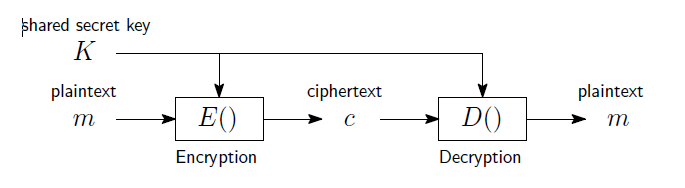
\includegraphics[height=13cm, width=13cm, keepaspectratio]{Immagini/Capitolo2/segreta_schema_blocchi.png}}
	\caption{Schema a blocchi crittografia a chiave segreta \label{fig:segreta_schema_blocchi}} 	
\end{figure}

\subsection{Impieghi crittografia a chiave segreta}
La crittografia a chiave segreta è alla base di molti meccanismi di sicurezza, i suoi principali impieghi sono: 
\begin{itemize}
  \item protezione della \textbf{confidenzialità} (l'uso classico di queste tecniche è rappresentato dalle \textbf{comunicazioni su un canale insicuro}, uno degli usi più moderni invece dalla \textbf{memorizzazione sicura su supporto insicuro})
  \item protezione dell'\textbf{integrità}: tramite queste tecniche possono essere eseguiti test per rilevare eventuali modifiche non consentite.
  \item autenticazione: tramite l'implementazione di protocolli per verificare l'identità di persone e/o processi.
\end{itemize}

\subsubsection{Comunicazioni su un canale insicuro}
In molte circostanze, due entità devono comunicare attraverso un canale insicuro correndo il rischio di essere ascoltate da una terza parte. Questo contesto è molto comune: si pensi alle reti LAN, che trasmettono dati in broadcast. La crittografia a chiave segreta permette a due entità che condividono un segreto (la chiave) di comunicare attraverso un canale insicuro, ove non può essere garantita l’assenza di intercettazioni/ascoltatori (eavesdropper), avendo la garanzia che il contenuto della comunicazione rimarrà confidenziale.

\subsubsection{Memorizzazione sicura}
Si supponga di disporre di un supporto di memorizzazione non protetto (ad esempio accessibile a molti utenti). Se si desidera salvare i dati proteggendone la confidenzialità si può definire una chiave segreta, salvare i dati dopo averli crittografati con tale chiave e custodire la chiave segreta in un luogo protetto. Il rischio dell'uso di questa tecnica consiste nella possibilità di smarrimento della chiave. In tal caso i dati sarebbero irrevocabilmente persi.

\subsubsection{Autenticazione forte}
Per \textbf{autenticazione forte (strong authentication)} si intende che si è in grado di provare la conoscenza di un segreto, che contraddistingue l'identità di una data entità, senza rivelarlo. L'autenticazione forte è ottenibile utilizzando la crittografia a chiave segreta, ed è particolarmente utile quando due processi devono comunicare su una rete insicura. A rigore il segreto che contraddistingue l'identità che si desidera autenticare dovrebbe essere noto solo a quest'ultima. Nella crittografia chiave segreta tale requisito non può essere soddisfatto. Il segreto in questione è una chiave crittografica che deve essere nota anche all'entità autenticante.

\subsubsection{Esempio}
Si supponga che Alice e Bob condividano una chiave segreta $K_{AB}$ e che vogliano autenticarsi reciprocamente, cioè ciascuno vuole accertarsi dell'identità dell'altro. \newline \textbf{ipotesi:} $K_{AB}$ è nota solo ad Alice e Bob. Alice deve dimostrare a Bob di conoscere $K_{AB}$ senza rivelarla e viceversa. \newline \textbf{Strategia a sfida e risposta:} ciascuno dimostra di conoscere $K_{AB}$ rispondendo ad una sfida posta dall'altro. La \textbf{sfida} è un numero/stringa random \textbf{r} non prevedibile e sempre diversa. La \textbf{risposta} alla sfida è la sfida stessa cifrata \textbf{$E(K_{AB},R)$}. In \figurename ~\ref{fig:strong_auth_sec} è riportato un possibile schema di autenticazione a sfida e risposta (challenge-response) a chiave segreta. La procedura segue i seguenti passi:
\begin{itemize}
  \item Alice genera un numero random $r_{A}$ (la sfida) e la invia al presunto Bob
  \item il presunto Bob critta la sfida con la sua chiave segreta $K'_{AB}$ e restituisce ad Alice la risposta $E(K'_{AB}, r_{A})$
  \item Alice riceve la risposta del presunto Bob e la decritta con la chiave $K_{AB}$, cioè calcola $D(K_{AB},E(K'_{AB}, r_{A}))$. Se ottiene $r_{A}$, allora il presunto Bob è realmente Bob poiché con elevatissima probabilità, se $D(K_{AB},E(K'_{AB}, r_{A})) = r_{A}$, allora $K'_{AB} = K_{AB}$. In caso negativo deduce invece che il presunto Bob è un impostore. In modo analogo Bob verifica l'identità di Alice.
\end{itemize}
\begin{figure}[htbp]
	\centering%
	\subfigure%
	{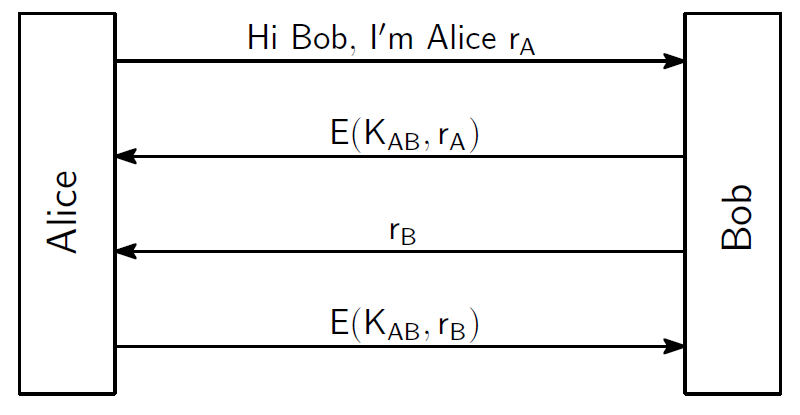
\includegraphics[height=13cm, width=13cm, keepaspectratio]{Immagini/Capitolo2/strong_auth_secret.png}}
	\caption{Schema a blocchi crittografia a chiave segreta \label{fig:strong_auth_sec}} 	
\end{figure}
La sicurezza del precedente protocollo si fonda sulle seguenti condizioni che non devono venire meno:
\begin{itemize}
  \item solo e soltanto Alice e Bob devono conoscere la chiave segreta $K_{AB}$
  \item le sfide generate devono essere \textbf{randomiche}, e di conseguenza non prevedibili, e \textbf{non ripetibili}, cioè la probabilità che due sfide si ripetano deve tendere a zero. L'attaccante potrebbe infatti collezionare molte coppie testo in chiaro/testo cifrato.
  \item è importante quindi che il numero di bit di una sfida sia superiore ad una data soglia (almeno 64 bit)
\end{itemize}

\subsubsection{Controllo di integrità}
La verifica dell’integrità di un messaggio inviato o di un file è un problema ricorrente in telecomunicazioni e in informatica. Per rilevare eventuali modifiche accidentali si fa uso generalmente di codici (somme) di controllo, detti anche \textbf{checksum}. Un \textbf{checksum} associa ad un qualsiasi messaggio $\textbf{m} \in \{0,1\}^*$ un codice di lunghezza prefissato di $b$ bit (generalmente $b = 32,64,128$ bit): $ck(\textbf{m}) \in \{0,1\}^b$. Un buon \textbf{checksum} dovrebbe variare in modo significativo anche a fronte di iminime variazioni dell'input. \newline \newline 
La sorgente del messaggio $m_{s}$ rende pubblico/invia il corrispondente checksum $ck(m_{s})$. Chi riceve il messaggio $m_{r}$ calcola il checksum e verifica se vale l'uguaglianza $ck(m_{s}) = ck(m_{r})$. In caso affermativo, conclude che $m_{s} = m_{r}$. Si noti tuttavia che, seppur improbabile, è possibile ottenere dei falsi positivi, cioè $ck(m_{s}) = ck(m_{r} )$ anche se non è vero.

\subsubsection{Checksum segreti e non segreti}
I codici di controllo servono per proteggere l’hardware da difetti e da inevitabili errori/guasti. Esistono codici di controllo molto sofisticati come i \textbf{CRC (Cyclic Redundancy Check)} per i quali la probabilità di falsi positivi è estremamente ridotta. Esistono anche i codici \textbf{FEC (Forward Error Correction)} che permettono di correggere eventuali errori oltre che a rilevarli (aggiungendo ulteriore ridondanza). Tuttavia entrambe queste tecniche \textbf{non} sono utilizzabili per la protezione contro attacchi intelligenti. Essendo pubblici, infatti, un avversario intelligente che vuole cambiare un messagio potrebbe modificare anche il codice di controllo in maniera coerente.\newline \newline
Per la protezione contro modifiche maliziose ad un messaggio, è richiesto un codice di controllo (checksum) segreto. Se l'algoritmo non è noto, nessuno può calcolare il checksum corretto per il messaggio modificato. Chiaramente, come nel caso degli algoritmi di cifratura, anziché un
algoritmo segreto conviene avere un algoritmo noto a tutti che richiede la conoscenza di una chiave segreta per il calcolo di un codice di controllo (Vedi pagina ~\pageref{sec:openStruct}, principio \textbf{Open Structure}). \newline \newline
In ciò consiste appunto un checksum cifrato, detto anche \textbf{MIC (Message Integrity Code)}. Il funzionamento del MIC è il seguente:
\begin{itemize}
  \item l'algoritmo produce un codice di autenticazione di lunghezza fissa $MIC(K,m)$, denominato anche \textbf{MAC (Message Authentication Code)}
  \item il codice MIC MIC(K,m) viene trasmesso insieme al messaggio m stesso
  \item formalmente l’input è una coppia $(K,m) \in \{0, 1\}^k \times \{0, 1\}^*$, dove $k$ denota il numero di bit della chiave segreta K, mentre l'output è sempre una stringa binaria di lunghezza prefissata, cioè $MIC(K,m) \in \{0, 1\}^b$
\end{itemize}

\subsection{Cifrari a blocchi e cifrari a flusso}
Un \textbf{cifrario a blocchi} elabora un blocco di elementi in ingresso per volta, producendo un blocco di uscita per ciascun blocco di ingresso. Questa metodologia implica quindi che:
\begin{itemize}
  \item il testo in chiaro deve essere preliminarmente suddiviso in blocchi
  \item il testo cifrato si ottiene combinando i vari blocchi cifrati
\end{itemize}
DES, IDEA e AES sono esempi di cifrari a blocchi simmetrici. Un \textbf{cifrario a flusso}, invece, elabora continuamente gli elementi in ingresso, producendo in uscita un "flusso" di elementi cifrati. Gli elementi cifrati vengono prodotti singolarmente, uno alla volta, man mano che la cifratura procede.

\section{Cifratura a blocchi}

\subsection{Introduzione e concetti generali}
L’algoritmo di cifratura converte un blocco di testo in chiaro in un blocco di testo cifrato. La chiave K non deve essere troppo corta (e.g. se K ha lunghezza 4 bit, sono sufficienti $2^4 = 16$ tentativi per individuarla). Analogamente la lunghezza (fissata) di un blocco non deve essere troppo piccola (e.g. se un blocco ha lunghezza 8 bit, ottenendo delle coppie plaintext - ciphertext si potrebbe costruire una tabella di $2^8 = 256$ coppie utilizzabile per la decfiratura).\newline 
D'altra parte, avere blocchi esageratamente lunghi oltre a non essere necessario dal punto di vista della sicurezza, comporta una gestione più complicata e può degradare le prestazioni. \textbf{64 bit è una lunghezza ragionevole per un blocco}: 
\begin{itemize}
  \item è improbabile ottenere ordine di $2^{64}$ coppie $\langle plaintext, ciphertext \rangle$ per costruire una tabella di decifratura, e
  \item anche se fosse possibile, la sua memorizzazione richiederebbe una spazio enorme ($2^{64}$ record da 64 bit),
  \item come pure l’ordinamento per consentire ricerche efficienti
\end{itemize}
Il modo più generale per cifrare un blocco da 64 bit è definire una \textbf{biiezione} $\gamma :\{0,1\}^{64} \rightarrow \{0,1\}^{64}$. Tuttavia, memorizzare la definizione della \emph{biiezione} in una struttura dati è impraticabile: sarebbero richiesti $2^84 \times 64 = 2^{70}$ bit. Ad essere precisi ce ne vogliono un po' di meno, trattandosi di un \textbf{biiezione}, comunque almeno $2^{69}$ bit sono richiesti \textcolor{red}{(perché?!?!)}. Inoltre, così facendo la chiave è incorporata nella biiezione: per renderla parametrica rispetto alla chiave è necessario memorizzare una biiezione per ogni possibile chiave.\newline \newline
I sistemi di crittografia a chiave segreta sono concepiti per usare una chiave ragionevolmente lunga (ad esempio 64 bit e generare una \textbf{biiezione} che appare, a chi non conosce la chiave, completamente \underline{random}. Se la biiezione fosse realmente random due input $i$ e $i'$ nei quali cambia un solo bit (uno qualunque) sarebbero \textbf{statisticamente indipendenti}: non può succedere, ad esempio, che il terzo bit dell'output cambia \textbf{sempre} quando il dodicesimo bit dell'input cambia. Gli algoritmi crittografici sono pensati per \textbf{diffondere/spargere} in tutti i bit dell'output il valore di ogni bit dell'input: si cerca di far si che ogni bit dell'output dipenda allo stesso modo da tutti i bit dell'input.

\subsection{Sostituzione e Permutazione}
Sostituzioni e permutazioni sono due trasformazioni base applicabili ad un blocco di dati.\newline \newline
Si assuma di dover cifrare un blocco di $k$ bit. Una \textbf{sostituzione} specifica, per ciascuno dei $2^k$ possibili valori dell'input, i $k$ bit dell'output. Per specificare una sostituzione \textbf{"completamente random"} sono necessari circa $k2^k$ bit. E' quindi impraticabile implementare una sostituzione per blocchi di $64$ bit, mentre è fattibile per blocchi di lunghezza di $8$ bit. Esempio di crittografia per sostituzione è il \textbf{Cifrario di Cesare}.\newline \newline
Una \textbf{permutazione} specifica, per ciascuna delle $k$ posizioni dei bit in input, la posizione del corrispondente bit nell'output. Per specificare una permutazione \textbf{"completamente random"} per un blocco di
lunghezza $k$ bit sono necessari $k\log_2 k$ bit. Infatti per ciascuno dei k bit va specificata la sua posizione nell'output; ogni posizione richiede $k\log_2 k$. Ad esempio: essendo $2^6 = 64$, sono necessari $6 = \log_2 {64}$ bit per specificare la nuova posizione che l'i-esimo bit in input avrà in output. \newline \newline
Si noti che una \textbf{permutazione} è un caso particolare di \textbf{sostituzione} in cui ogni bit dell'output ottiene il suo valore da esattamente un bit dell'input.

\subsection{Cifrario a blocchi – schema generale}
Un algoritmo di cifratura a chiave segreta può funzionare come segue:
\begin{itemize}
  \item scompone il blocco in input in pezzi più piccoli (e.g. blocchi da 8 bit)
  \item applica una sostituzione (tramite una \textbf{rete combinatoria}) a ciascun pezzo da 8 bit (la sostituzione dipenderà dal valore della chiave)
  \item gli output delle sostituzioni vengono riuniti in un unico blocco (64 bit)
  \item tale blocco viene permutato in un permutatore a 64 bit (che ha il compito di diffondere le modifiche eseguite nelle sostituzioni)
  \item il processo viene ripetuto un certo numero di volte riportando l'output in ingresso
\end{itemize}
%%La scomposizione in blocchi e la ricomposizione vanno effettuate in maniera saggia, al fine di ottimizzare %%efficacia e efficienza del \textbf{cifrario}.
\subsection{Cifrario a blocchi – esempio}
Ogni attraversamento del cifrario viene detto \textbf{round}. In riferimento alla \figurename ~\ref{fig:block_chipher} si fanno le seguenti considerazioni. Con un solo round, un bit $b_x$ di input può influenzare soltanto 8 bit $b_{x1}, b_{x2}, …, b_{x8}$ dell'output, poiché $b_x$ ha attraversato soltanto un blocco di sostituzione. In generale i bit $b_{x1}, b_{x2}, …, b_{x8}$ non sono consecutivi essendo stati mescolati nel permutatore. Alla fine del secondo round, assumendo che i bit $b_{x1}, b_{x2}, …, b_{x8}$ siano smistati in blocchi di sostituzione distinti, il bit $b_x$ iniziale influenza tutti i bit in output.
\begin{figure}[htbp]
	\centering%
	\subfigure%
	{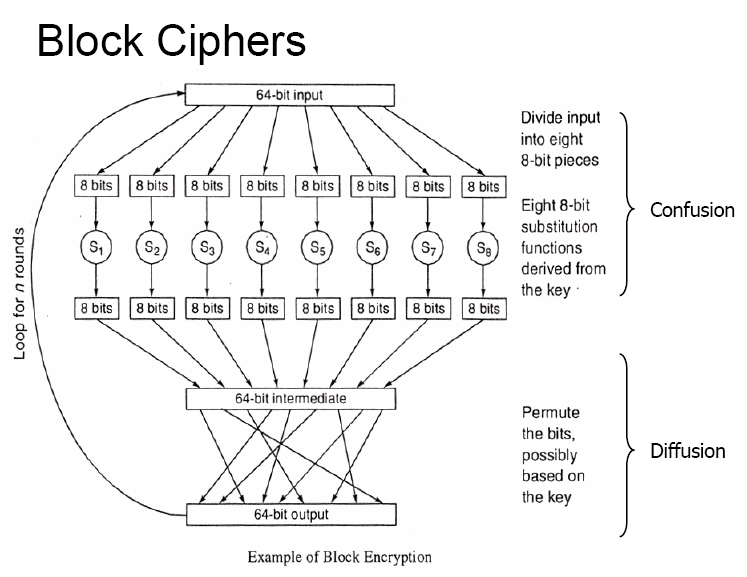
\includegraphics[height=13cm, width=13cm, keepaspectratio]{Immagini/Capitolo2/block_cipher.png}}
	\caption{Schema a blocchi crittografia a chiave segreta \label{fig:block_chipher}} 	
\end{figure}

\section{Data Encryption Standard - DES}
DES fu pubblicato nel 1977 dal \textbf{National Bureau of Standards}, ora rinominato \textbf{N}ational \textbf{I}nstitute of \textbf{S}tandards and \textbf{T}echnology (\textbf{NIST}), per usi commerciali e "altre" applicazioni del governo statunitense. Progettato da IBM, si basa sul precedente cifrario \textit{Lucifer} ed è frutto della collaborazione con consulenti della NSA. DES usa una chiave di 56 bit, e mappa un blocco di input da 64 bit in un blocco di output da 64 bit (l'algoritmo è quindi abbastanza rigido, al contrario di altri cifrari a blocchi). La \textbf{chiave} è in realtà costituita da una sequenza di 64 bit, ma un bit in ogni ottetto (il blocco da 64 bit è formato da 8 sequenze di 8 bit dette ottetti) è usato come \textbf{odd parity} su ciascun ottetto. Di fatto, soltanto 7 bit in ogni ottetto sono quindi veramente significativi come chiave. \newline \newline

DES è efficiente se realizzato in hardware, ma relativamente lento se implementato in software. Sebbene l'essere difficilmente implementabile come software non fosse un requisito specificato nel progetto molti sostengono che in realtà questa mancanza fosse voluta, forse per limitarne l'uso ad organizzazioni in grado di realizzare sistemi hardware, o forse perché rese più facile controllare l'accesso alla tecnologia. Ad ogni modo, l'aumento delle capacità di calcolo delle CPU rese possibile realizzare una versione software di DES. Una 500-MIPS (Million Instruction Per Second) CPU può infatti cifrare ad un tasso di circa 30 KB/s e forse più, a seconda dei dettagli architetturali della CPU e dell'intelligenza dell'implementazione. Un processore Intel Core i7 Extreme Edition i980EE ha una capacità di calcolo di circa 150 MIPS, quindi può cifrare ad un tasso di circa 9 KB/s (per cifrare 1 MB impiega circa 110 secondi). L’implementazione software è pertanto attualmente adeguata a molte applicazioni.\newline \newline


\subsection{Violabilità e sicurezza di DES}

\subsubsection{Perché chiavi da 56 bit?}
La scelta di una chiave da 56 bit causò molte controversie. Prima che DES fu adottato, le persone al di fuori della \textit{intelligence community} lamentavano che 56 bit non offrivano una sicurezza adeguata. Perché solo 56 dei 64 bit di una chiave DES sono effettivamente usati nell'algoritmo? Lo svantaggio di usare 8 bit della chiave per un controllo di parità è che ciò rende DES molto meno sicuro (256 volte meno sicuro contro una ricerca esaustiva). Ma qual è il vantaggio di usare 8 bit per un controllo di parità? Una possibile risposta è che permette di verificare che la chiave non sia corrotta. Tuttavia questa spiegazione non regge. Se si considerassero infatti 64 bit a caso invece della chiave, c'è una probabilità su 256 che il controllo di parità dia esito positivo. La probabilità che la chiave sia comunque errata (nonostante il controllo di parità dia esito positivo) è troppo alta. Inoltre avere una chiave corrotta non comporta un problema di sicurezza, semplicemente la cifratura/decifratura non viene eseguita correttamente. Chiaramente è anche ridicolo sostenere che la scelta di 56 bit sia stata fatta per risparmiare memoria. \newline La risposta ormai condivisa è che il governo statunitense abbia deliberatamente indebolito la sicurezza di DES di una quantità appena sufficiente da consentire alla NSA di violarlo.

Gli avanzamenti tecnologici dell'industria dei semiconduttori hanno reso ancora più critico il problema della lunghezza della chiave di DES. la velocità dei chip e un po' di furbizia permettono di violare (individuare) le chiavi DES con approcci a forza bruta in tempi ragionevoli. Il rapporto prestazioni/prezzo dell'hardware cresce del
$40\%$ per anno. La lunghezza delle chiavi dovrebbe aumentare di 1 bit ogni 2 anni. Assumendo che 56 bit erano appena sufficienti nel 1979 (quando DES fu standardizzato), 64 bit erano adeguati nel 1995, e 128 bit dovrebbero essere sufficienti fino al 2123. \newline \newline Ragioniamo ora sulla sicurezza di DES. Se si dispone di un singolo blocco $\langle plaintext,ciphertext \rangle$ quanto è difficile trovare la chiave? Un approccio a forza bruta dovrebbe provare ordine di $2^{56} \approx 10^{17}$ chiavi. Se ogni tentativo richiede una singola istruzione sono necessarie ordine di 1000 MIPS-year istruzioni.
\begin{itemize}
  \item 1 MIPS = 1 Milionef di Istruzioni Per Secondo
  \item 1 MIPS-year = numero di istruzioni eseguite in un anno ad un tasso pari a 1 MIPS
  \item 1 MIPS-year = 1 MIPS $\times(365 \times 86400)$ secondi in un anno = $3,1536 \times 10^{13}$ istruzioni
  \item $2^{56} \approx 10^{17} \approx 10^{3}$ MIPS-year
\end{itemize}
Questo vale tuttavia \textbf{SOLO} per effettuare una ricerca esaustiva. Dopo di che entra in gioco il fatto che io sappia riconoscere o meno il testo in chiaro.
\subsubsection{Violabilità DES - esempio}
Anche nell'ipotesi più scomoda per l'avversario di disporre solo di testo cifrato (in ragionevole quantità), un attacco a forza bruta è ancora possibile. Se ad esempio l'avversario sa soltanto che il testo in chiaro è ASCII a 7 bit ogni volta che prova una chiave deve verificare se sono nulli tutti i bit nelle posizioni $8, 16, 24, ..., n \times 8, ...$. Per ogni blocco di 64 bit, vanno esaminati solo 8 bit; i bit in posizione 8, 16, 24, 32, 40, 48, 56, 64. Se almeno uno di questi bit vale 1 la chiave è sicuramente errata. in caso contrario nulla si può dire; \textbf{la probabilità di errore è pertanto 1 su 256 ossia la probabilità che tutti questi bit valgano 0}. Se l'avversario esamina diversi blocchi, ad esempio 10, e verifica che si tratta sempre di ASCII a 7 bit la probabilità che la chiave scelta sia errata si riduce a 1 su 2560. Si noti che gli attuali chip commerciali che implementano DES non si prestano a ricerche esaustive della chiave: sono pensati per cifrare molti dati con una stessa chiave. Infatti il caricamento di una chiave è un'operazione lenta se confrontata con la velocità con la quale viene eseguita la cifratura dei dati. Tuttavia è sempre possibile costruire un chip ottimizzato ad eseguire ricerche esaustive della chiave.

\subsubsection{Violabilità DES - cifratura multipla}
Per ovviare a tali problemi di sicurezza è possibile cifrare più volte e con diverse chiavi lo stesso blocco di dati. Si parla di \textbf{cifratura multipla (multiple encryption)}. Si ritiene che una cifratura con un triplo DES sia
$2^{56}$ volte più difficile da violare.

\subsection{Funzionamento DES}
\subsubsection{Struttura base}
\begin{figure}[htbp]
	\centering%
	\subfigure%
	{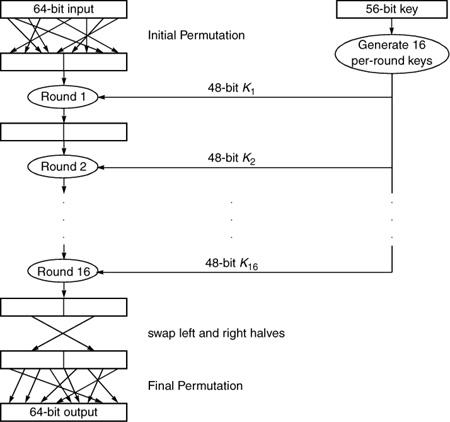
\includegraphics[height=10cm, width=13cm, keepaspectratio]{Immagini/Capitolo2/des_structure.png}}
	\caption{Schema a blocchi DES \label{fig:des_struct}} 	
\end{figure}
La struttura di base dell'algoritmo DES è descritta in \figurename ~\ref{fig:des_struct}. In estrema sintesi:
\begin{itemize}
  \item L'input di 64 bit è sottoposto ad una permutazione iniziale;
  \item La chiave da 56 bit viene usata per generare 16 per-round chiavi da 48 bit; una chiave per ciascuno dei 16 round, prendendo 48 differenti sottoinsiemi dei 56 bit della chiave
  \item Ogni round riceve in input l'output di 64 bit del round precedente e la chiave da 48 bit di quel round
  \item Ogni round restituisce un output di 64 bit
  \item Dopo il 16-esimo round, le due metà dell'output di 64 bit vengono scambiate e il risultato viene sottoposto ad un’altra permutazione (inversa a quella iniziale)
  \item La decifratura consiste semplicemente nell’eseguire la cifratura DES all’indietro
  \item Per decifrare un blocco è necessario applicare la permutazione iniziale (ciò annulla l’effetto della permutazione finale), generare le 16 chiavi di round, che andranno usate in ordine inverso (prima $K_{16}$, l'ultima chiave generata), seguire 16 round esattamente come nella cifratura, scambiare le due metà dell'output e sottoporle a un'altra permutazione (che annulla l'effetto della permutazione iniziale)
\end{itemize}
Per descrivere DES è quindi sufficiente discutere le permutazioni iniziale e finale, come le chiavi di round sono generate, e cosa succede durante un round.


\subsubsection{Permutazioni dei dati}
L'operazione di permutazione è molto importante in quanto diffonde la dipendenza dei bit in/out. Nel caso di DES però le permutazioni finale e iniziale non hanno effetto. Dimostriamo tale affermazione. \newline
\begin{figure}[htbp]
	\centering%
	\subfigure%
	{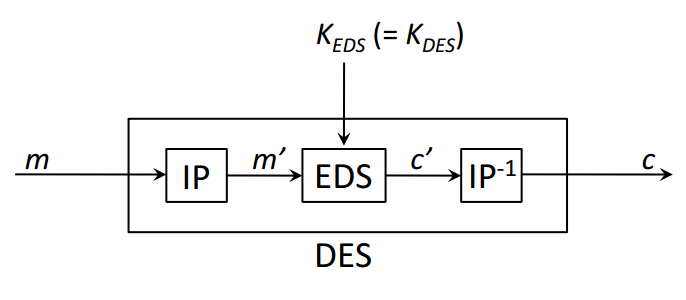
\includegraphics[height=10cm, width=8cm, keepaspectratio]{Immagini/Capitolo2/des_perm_3.png}}
	\caption{Inutilità delle permutazioni iniziale e finale \label{fig:des_perm_3}} 	
\end{figure}
Supponiamo di non averle. Se assumiamo per assurdo che il cifrario cosi ottenuto sia facile da violare, vogliamo dimostrare che anche DES è facile da violare. Chiamiamo il cifrario senza permutazione EDS. Se posso violare EDS (disponendo, ad esempio, di una coppia $\langle plaintext, ciphertext \rangle$), basta permutare ciò che ottengo e violo DES. Infatti, sia $\langle m, c \rangle$ una coppia $\langle plaintext, ciphertext \rangle$ di DES. Si consideri allora la coppia $\langle m', c' \rangle$, dove m' e c' sono ottenuti applicando la permutazione iniziale ad m e c. Allora, la chiave $K_{EDS}$ che si ottiene violando EDS per la
coppia $\langle m', c' \rangle$ coincide con la chiave $K_{DES}$ di DES per la
coppia $\langle m, c \rangle$ (vedi \figurename ~\ref{fig:des_perm_3}). L'ipotesi è che tali permutazioni siano state introdotte per rendere più complicata una possibile implementazione software.
\begin{figure}[htbp]
	\centering%
	\subfigure%
	{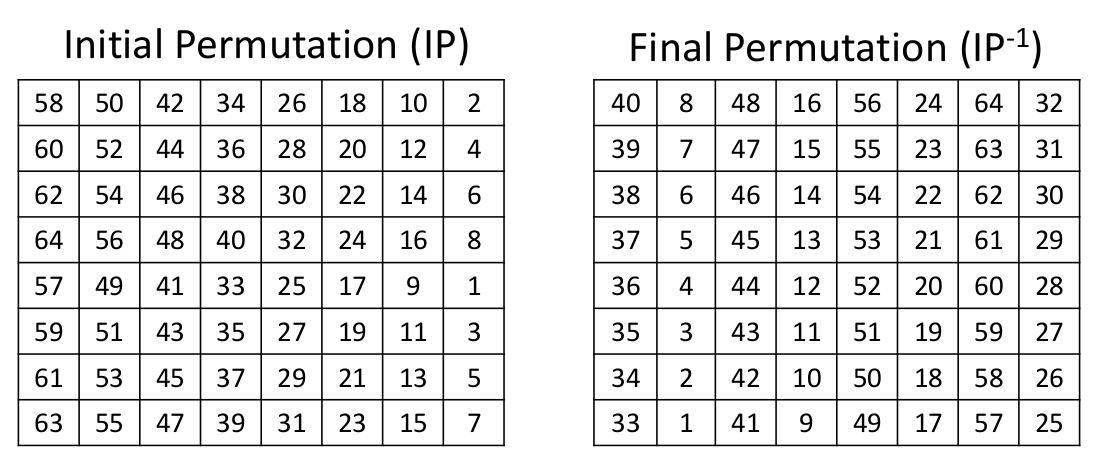
\includegraphics[height=10cm, width=13cm, keepaspectratio]{Immagini/Capitolo2/des_perm.png}}
	\caption{Tabella permutazioni DES \label{fig:des_perm}} 	
\end{figure}
Come sono state definite quindi le permutazioni iniziale e finale? E' di fatto una permutazione regolare, come è mostrato in \figurename ~\ref{fig:des_perm}. Le tabelle vanno interpretate nel seguente modo: i numeri, da 1 a 64, riportati in tabella rappresentano le posizioni dei bit in input alla permutazione, mentre l’ordine (per righe da sx verso dx) dei numeri nella tabella rappresenta la corrispondente posizione dei bit in output. Ad esempio, la permutazione iniziale sposta il 58-esimo bit in input nel primo bit in output, e il 50-esimo bit in input nel secondo bit in output. Non si tratta di permutazioni generate in modo random, in quanto presenta delle evidenti regolarità, come è evidenziato in \figurename ~\ref{fig:des_perm_2}.
\begin{figure}[htbp]
	\centering%
	\subfigure%
	{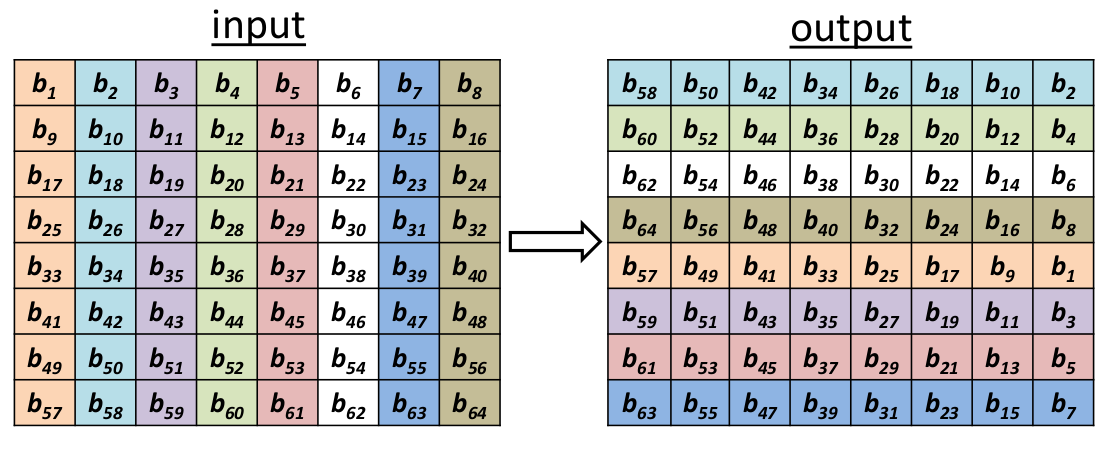
\includegraphics[height=10cm, width=10cm, keepaspectratio]{Immagini/Capitolo2/des_perm_2.png}}
	\caption{Regolarità tabella permutazioni DES \label{fig:des_perm_2}} 	
\end{figure}
\subsubsection{Generazione chiavi di round}
DES genera sedici chiavi di round da 48 bit a partire dalla chiave principale K di 64 bit nominali, di cui solo 56 effettivi. I bit di parità di K non vengono infatti considerati. Denoteremo con $K_{1}$,$K_{2}$,...,$K_{16}$ le sedici chiavi di round. Il procedimento è il seguente:
\begin{itemize}
  \item viene prima effettuata una permutazione iniziale sui 56 bit effettivi di K
  \item i 56 bit in output vengono divisi in due metà $C_{0}$ e $D_{0}$
  \item Le sedici chiavi vengono generate in sedici round, i.e. nell'i-esimo round viene generata la chiave di round $K_{i}$
\end{itemize}
\subsubsection{Permutazione iniziale}
\begin{figure}[htbp]
	\centering%
	\subfigure%
	{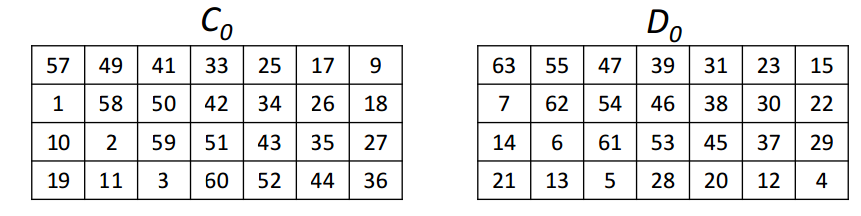
\includegraphics[height=10cm, width=10cm, keepaspectratio]{Immagini/Capitolo2/des_perm_keys.png}}
	\caption{Permutazione iniziale della chiave \label{fig:des_perm_keys}} 	
\end{figure}
\begin{figure}[htbp]
	\centering%
	\subfigure%
	{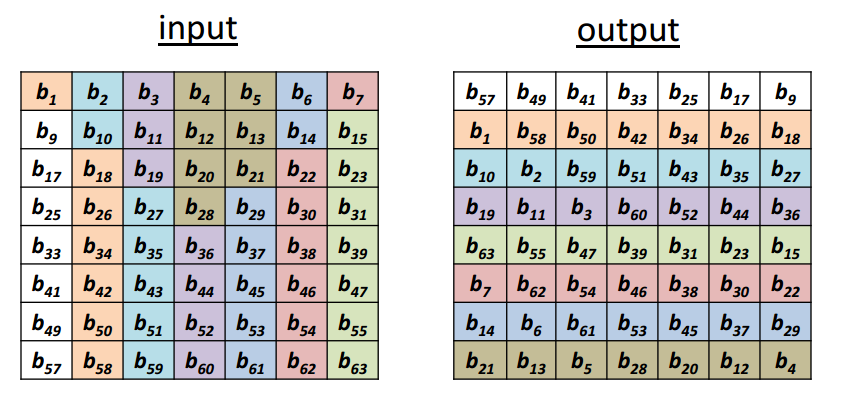
\includegraphics[height=10cm, width=10cm, keepaspectratio]{Immagini/Capitolo2/des_perm_keys_2.png}}
	\caption{Regolarità tabella permutazioni delle chiavi DES \label{fig:des_perm_keys_2}} 	
\end{figure}
La struttura della permutazione iniziale della chiave è illustrata in \figurename ~\ref{fig:des_perm}. Il valore numerico di un elemento della tabella rappresenta la posizione del bit in input, mentre l’ordine nella tabella rappresenta la posizione del bit in output (come per le permutazioni dei dati). Anche in questo caso non è random, in quanto presenta delle evidenti regolarità, come è evidenziato in \figurename ~\ref{fig:des_perm_keys_2}. Come nel caso delle permutazioni iniziale e finale dei dati, non apportano alcun miglioramento alla sicurezza.
\newpage
\subsubsection{Generazione $K_{i}$ nell'i-esimo round}
\begin{figure}[htbp]
	\centering%
	\subfigure%
	{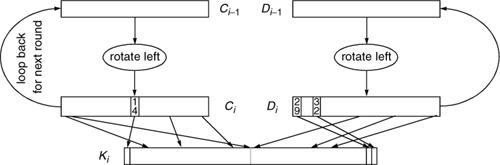
\includegraphics[height=10cm, width=10cm, keepaspectratio]{Immagini/Capitolo2/round_i.png}}
	\caption{generazione di Ki: round i \label{fig:round_i}} 	
\end{figure}
Trattiamo ora la generazione della chiave $K_{i}$ che avviene nell'i-esimo round. La procedura avviene seguendo questi passi (come mostrato in \figurename ~\ref{fig:round_i}):
\begin{itemize}
  \item i bit delle due metà $C_{i-1}$ e $D_{i-1}$ della (i-1)-esima chiave $K_{i-1}$ vengono ruotati (traslazione ciclica) a sinistra. L'entità della traslazione a dipende dal round: nei round 1, 2, 9 e 16 si ha una rotazione a sinistra di un solo bit (i.e. il primo bit diventa l’ultimo bit a destra), mentre negli altri round si ha una rotazione a sinistra di due bit.
  \item la permutazione di $C_{i}$ che produce la metà sinistra di $K_{i}$ è illustrata sotto. Si noti che i bit in posizione 9, 18, 22, e 25 sono scartati.
  	\begin{table}[h]
  	\centering
	\begin{tabular}{llllll}
	14 & 17 & 11 & 24 & 1  & 5  \\
	3  & 28 & 15 & 6  & 21 & 10 \\
	23 & 19 & 12 & 4  & 26 & 8  \\
	16 & 7  & 27 & 20 & 13 & 2 
	\end{tabular}
	\end{table}
  \item la permutazione di $D_{i-1}$ ruotato, cioè di $D_{i}$ , che produce la metà destra di $K_{i}$ è illustrata sotto. Si noti che i bit in posizione 35, 38, 43, e 54 sono scartati; rimangono così 24 bit anziché 28.
  	\begin{table}[h]
  	\centering
	\begin{tabular}{llllll}
	41 & 52 & 31 & 37 & 47 & 55  \\
	30 & 40 & 51 & 45 & 33 & 48 \\
	44 & 49 & 39 & 56 & 34 & 53  \\
	46 & 42 & 50 & 36 & 29 & 32 
	\end{tabular}
	\end{table}
\end{itemize}
\subsubsection{Un round di DES}
\begin{figure}[htbp]
	\centering%
	\subfigure%
	{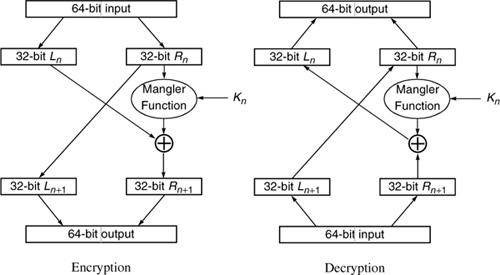
\includegraphics[height=10cm, width=9cm, keepaspectratio]{Immagini/Capitolo2/round_des.png}}
	\caption{Struttura di un round di DES \label{fig:round_des}} 	
\end{figure}
La struttura di un round di des è illustrata in \figurename ~\ref{fig:round_des}). I 64 bit in input sono divisi in due metà da 32 bit: $L_{n}$, la metà sinistra dopo l'(n-1)-esimo round, e $R_{n}$, la metà destra dopo l'(n-1)-esimo round. L'output di 64 bit del round si ottiene concatenando le due metà: $L_{n + 1}$, la metà sinistra dopo l'n-esimo round, e $R_{n + 1}$, la metà destra dopo l'n-esimo round. $L_{n+1}$ è semplicemente $R_{n}$, mentre $R_{n + 1}$ è ottenuto come segue:
\begin{itemize}
  \item $R_{n}$ e $K_{n}$ sono posti in input alla mangler function; la mangler function viene anche detta funzione di Feistel
  \item l'output della mangler function, $mangler(R_{n}, K_{n})$, è una quantità di 32 bit; si noti che $R_{n}, K_{n}$ sono composti da
32 e 48 bit rispettivamente
  \item l'output $mangler(R_{n}, K_{n})$ viene poi sommato (XOR) con $L_{n}$
  \item il risultato ottenuto è $R_{n+1} = mangler(R_{n}, K_{n}) \oplus L_{n}$
\end{itemize}
Si noti che ogni round di DES è facilmente invertibile: noti $L_{n+1}$ , $R_{n+1}$ e $k_{n}$ è facile ottenere $L_{n}$ e $R_{n}$. Infatti $R_{n} = L_{n+1}$ e, poiché $R_{n+1} = mangler(R_{n}, K_{n}) \oplus L_{n}$, risulta $R_{n+1} \oplus mangler(R_{n}, K_{n}) = L_{n}$ (in virtù della proprietà dello XOR secondo cui $x \oplus y \oplus y = x$). La mangler function non è quindi mai utilizzata in senso inverso. DES è elegantemento progettato in modo da essere facilmente invertibile senza richiedere l'invertibilità della mangler function. Esaminando attentamente la \figurename ~\ref{fig:round_des}), si evince che la decifratura è di fatto identica alla cifratura, tranne per il fatto che le due metà da 32 bit sono invertite. In altre parole, fornendo $R_{n+1} \mid L_{n+1}$ in input al round n si ottiene $R_{n} \mid L_{n}$ in uscita
\subsubsection{Mangler Function}
\begin{figure}[htbp]
	\centering%
	\subfigure%
	{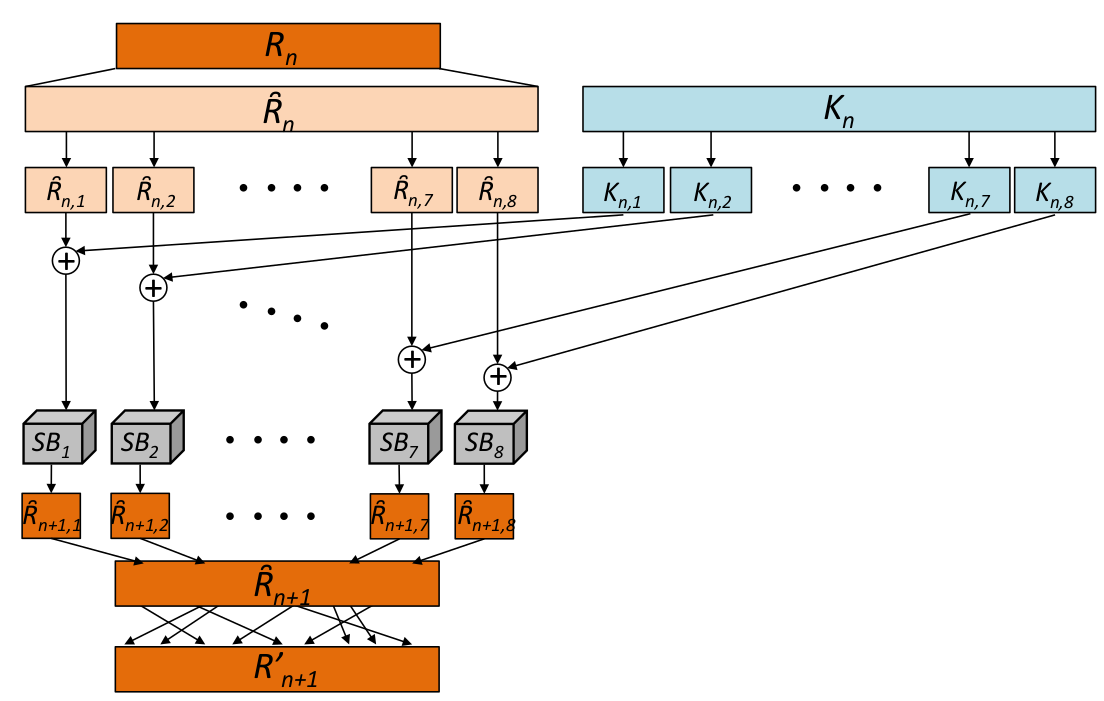
\includegraphics[height=11cm, width=11cm, keepaspectratio]{Immagini/Capitolo2/mangler.png}}
	\caption{Mangler function \label{fig:mangler}} 	
\end{figure}
La mangler function prende in input i 32 bit di $R_{n}$, o R per semplificare, e i 48 bit della chiave $K_{n}$ , o K per semplificare. Produce un output da 32 bit che sommato (XOR) con $L_{n}$ permette di ottenere $R_{n+1}$ (il prossimo R).\newline
La prima operazione è l’espansione di R, da 32 bit a 48 bit. R è scomposto in otto pezzi da 4 bit $R = \lbrace r_{1} , r_{2}, ..., r_{8} \rbrace$. L’i-esimo pezzo $r_{i}$ viene espanso a 6 bit aggiungendo in testa e in coda rispettivamente l’ultimo bit di $r_{i-1}$ e il primo bit di $r_{i+1}$. $r_{1}$ e $r_{8}$ sono considerati adiacenti, cioè $r_{0} = r_{8}$ e $r_{9} = r_{1}$. (Fare riferimento alla \figurename ~\ref{fig:mangler_exp})).
\begin{figure}[htbp]
	\centering%
	\subfigure%
	{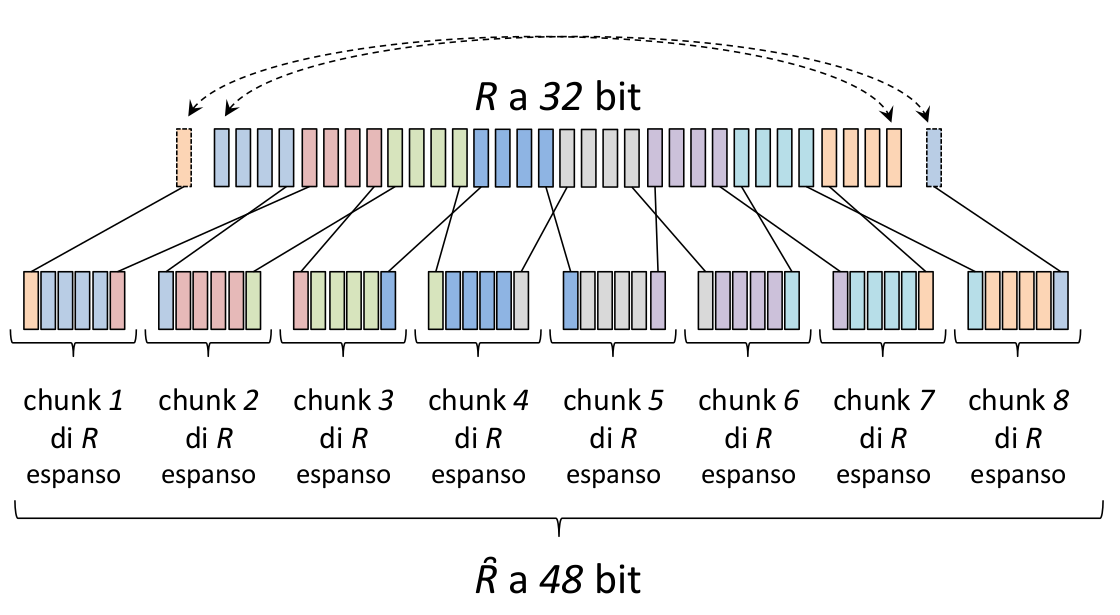
\includegraphics[height=11cm, width=11cm, keepaspectratio]{Immagini/Capitolo2/mangler_exp.png}}
	\caption{Mangler function - espansione \label{fig:mangler_exp}} 	
\end{figure}
\newline
la chiave K($K_{n}$) viene scomposta in otto chunk (pezzi) da 6 bit. L'i-esimo chunk di R($R_{n}$) espanso viene sommato (XOR) all’i-esimo chunk di K. L'output a 6 bit ottenuto viene sottoposto ad una sostituzione \textbf{S-box} che produce un output di 4 bit. Vi sono in tutto otto S-box distinte; l’i-esima S-box elabora la somma dell’i-esimo chunk di K e di R. Ogni S-box ha 64 possibili input e 16 possibili output. Ovviamente input diversi possono essere mappati nello stesso output (sto riducendo lo spazio). Le S-box sono definite in modo tale che esattamente quattro
input distinti sono mappati in ciascun output possibile. Ogni S-box può riguardarsi come quattro S-box separate aventi 4 bit sia in input che in output: i quattro bit in input corrispondono ai bit interni (dal secondo al quinto) dell'input globale, e i due bit esterni (primo e sesto) dell’input globale servono a selezionare quale dei quattro output ottenuti rappresenta l'output globale.
\begin{figure}[htbp]
	\centering%
	\subfigure%
	{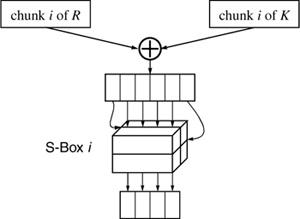
\includegraphics[height=7cm, width=7cm, keepaspectratio]{Immagini/Capitolo2/sbox.png}}
	\caption{S-Box \label{fig:sbox}} 	
\end{figure}
Infine gli otto output, da 4 bit, delle otto S-box sono riuniti in un unico output a 32 bit che viene sottoposto ad una permutazione. Tale permutazione aumenta il livello di sicurezza perché le sostituzioni fatte in ciascuna S-box in un round di DES vengono diffuse negli input di più S-box nel round seguente. Senza tale permutazione, un bit nella parte sinistra dell'input influenzerebbe principalmente alcuni bit della parte sinistra dell'output. Tale permutazione è mostrata in \figurename ~\ref{fig:sbox_perm}).
\begin{figure}[htbp]
	\centering%
	\subfigure%
	{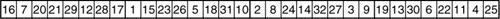
\includegraphics[height=2cm, width=10cm, keepaspectratio]{Immagini/Capitolo2/sbox_perm.png}}
	\caption{Permutazione output S-Box \label{fig:sbox_perm}} 	
\end{figure}
	
\section{Advanced Encryption Standard - AES}
AES fu introdotto perché DES aveva una chiave troppo corta, 3DES (triplo DES) era troppo lento e IDEA era protetto da un brevetto, ed era in parte sospetto e lento. Il NIST si impegnò quindi a sviluppare un nuovo standard. Non si trattava di un problema solo tecnico, ma anche di un problema politico, poiché alcuni rami del governo avevano ostacolato il più possibile la diffusione e l'esportazione della crittografia sicura, e il fatto che il governo appoggiasse il NIST era visto con scetticismo, e molti non si fidavano. Il NIST voleva realmente creare un nuovo standard di sicurezza eccellente, cioè efficiente, flessibile, sicuro e free (non protetto). \newline

Nel 1997 il NIST annunciò una gara per la selezione di un nuovo standard di cifratura destinato a proteggere informazioni governative sensibili. Dopo molti anni di studio e discussioni, il NIST scelse l'algoritmo \textbf{Rijndael}, proposto da due crittografi belgi Joan Daemen e Vincet Rijmen. Rijndael prevede diverse lunghezze per i blocchi e
per la chiave: 128, 160, 192, 224, e 256 bit. La lunghezza di un blocco e quella della chiave possono differire. Il 26 Novembre 2001, viene emanato \textbf{AES}, una standardizzazione di Rijndael. AES quindi consiste in \textbf{un'implementazione di Rijndael} con determinati parametri. Lo standard AES, infatti:
\begin{itemize}
  \item fissa la lunghezza dei blocchi a 128 bit
  \item la chiave può essere di 128, di 192 o di 256 bit. Si parla di \textbf{AES-128}, \textbf{AES-192} e \textbf{AES-256}
\end{itemize}

Nel seguito si descriverà Rijndael, specificando di volta in volta i parametri di AES. A grandi linee, Rijndael somiglia a DES e a IDEA. Ci sono più round che "strapazzano" un blocco di testo in chiaro per ottenere il corrispondente cifrato, e c'è un algoritmo per l'espansione della chiave; a partire dalla chiave segreta genera le chiavi da usare nei vari round.

\subsubsection{Rijndael/AES - parametri}
Rijndael ha una struttura flessibile grazie all'uso di due parametri indipendenti, e di un terzo parametro derivato dai primi due:
\begin{itemize}
  \item $N_{b}$ \textbf{dimensione di un blocco}: numero di parole (word) da 32 bit (colonne da 4 ottetti) in un blocco da cifrare. In AES $N_{b = 4}$, ovvero un blocco ha lunghezza 128 bit, ovvero 4 parole da 32 bit (4 colonne da 4 ottetti).
  \item $N_{k}$ \textbf{dimensione della chiave}: numero di parole (word) da 32 bit (colonne da 4 ottetti) in una chiave di cifratura. In AES-128 $N_{k} = 4$, In AES-192 $N_{k} = 6$, In AES-256 $N_{k} = 8$. In Rijndael $N_{k}$ può essere un qualsiasi intero tra 4 e 8.
  \item $N_{r}$ \textbf{numero di round}: questo parametro dipende da $N_{b}$ e da $N_{k}$. Come idea generale, più lunga è la chiave più round sono necessari per rendere la violazione della cifratura difficile quanto un attacco a forza bruta sulla chiave. Inoltre il numero di round deve aumentare all'aumentare della lunghezza di un blocco (e della chiave); ogni bit del testo in chiaro (e della chiave) deve influenzare (in modo complesso) ciascun bit del testo cifrato. Rijndael specifica che $N_{r}$ = 6 + max($N_{b}$ ,$N_{k}$). In AES-128 $N_{r} = 10$, in AES-192 $N_{r} = 12$, in AES-256 $N_{r} = 14$.
\end{itemize}
  
\subsubsection{Array di stato}
Rijndael mantiene un array di stato rettangolare durante il funzionamento. Ogni elemento dell'array è un ottetto. Complessivamente ci sono $N_{b}$ colonne da 4 ottetti. Lo stato iniziale è ottenuto popolando l’array, colonna per colonna, mediante le $N_{b}$ colonne da 4 ottetti che costituiscono il blocco di input. \\

Durante gli $N_{r}$ round lo stato viene modificato e il blocco di output dell'algoritmo si ottiene leggendo colonna per colonna lo stato finale. \\

La struttura base di Rijndael è mostrata in \figurename ~\ref{fig:Rij_struct}.Prima del primo round, tra i vari round, e dopo il round $N_{r}$ viene eseguito l'or-esclusivo ($\oplus$ XOR) del contenuto dell'array di stato, con i prossimi $4\cdot N_{b}$ ottetti della \textbf{chiave espansa}. Gli ottetti della chiave espansa vengono letti per colonna in modo da formare un matrice di $N_{b}$ colonne da 4 ottetti ciascuna. I primi $N_{r} – 1$ round comprendono una sequenza di operazioni identiche, mentre il round $N_{r}$ ne omette una.

\begin{figure}[htbp]
	\centering%
	\subfigure%
	{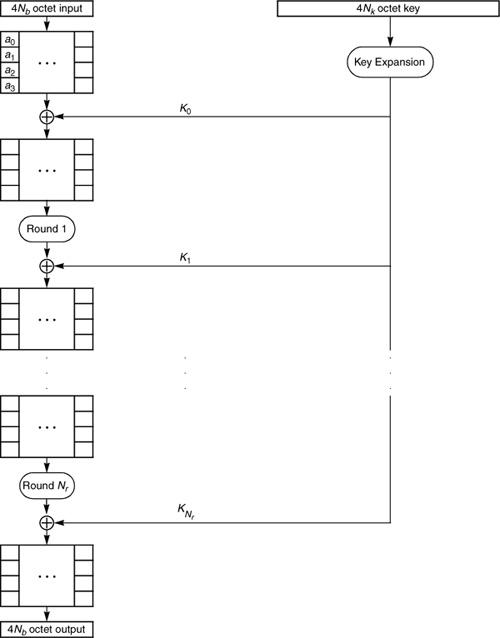
\includegraphics[height=13cm, width=10cm, keepaspectratio]{Immagini/Capitolo2/rijndael_struttura.png}}
	\caption{Struttura di base di Rijndael \label{fig:Rij_struct}} 	
\end{figure}

\subsubsection{Espansione della chiave}
La chiave segreta di Rijndael è un blocco formato da $4 \cdot N_{k}$ ottetti ($N_{k}$ word da 32 bit). L'algoritmo di espansione della chiave scandisce la chiave in modo da ottenere $N_{k}$ colonne da 4 ottetti, poi espande la matrice ottenuta introducendo delle colonne (da 4 ottetti) aggiuntive (avvalendosi dello stesso tipo di operazioni primitive usate durante i round, che verrano descritte in seguito). L'espansione si arresta quando si hanno complessivamente $(N_{r} + 1)N_{b}$ colonne, ovvero l'esatta quantità di chiavi espanse. Non tratteremo qui nel dettaglio come avviene l'espansione, per l'approfondimento si rimanda a testi dedicati.\\

\textbf{Numerazioni}: righe, colonne, e chiavi di round sono numerate a
partire 0, mentre i round sono invece numerati a partire da 1.

\subsubsection{Operazioni primitive}
Rijndael utilizza quattro operazioni primitive, sia nell'espansione della chiave che all'interno dei round:
\begin{itemize}
  \item \textbf{OR-esclusivo ($\oplus$ XOR)}, in cui sono coinvolte le chiavi espanse
  \item \textbf{sostituzione di byte}, chiamata \textbf{S-box}. Si tratta di una sostituzione ottetto-per-ottetto (byte-per- byte) definita da una specifica tabella, che specifica, per ciascuno dei possibili 256 byte in input il corrispondente byte in output tra i 256 possibili. Per la rappresentazione della tabella fa comodo usare la notazione esadecimale in cui, ad esempio, FC rappresenta il 252-esimo byte. Un'esempio di S-box è mostrato in \figurename ~\ref{fig:Rij_sbox}.
  \item \textbf{scorrimento circolare di ottetti (byte)} di una riga o di una colonna pari a un qualche numero di celle
  \item mescolamento colonne, \textbf{MixColumn}. Consiste nella sostituzione di una colonna di 4 ottetti con un'altra colonna di 4 ottetti. MixColumn può essere implementata con una singola tabella contenente 256 colonne di 4 ottetti: ciascuno dei 4 ottetti in una colonna di input è usato come un indice per recuperare una colonna dalla tabella. Ogni colonna recuperata dalla tabella è ruotata (scorrimento verticale circolare dall'alto in basso) verticalmente in modo tale che il suo ottetto in cima sia posto nella stessa riga dell’ottetto di input, e le quattro colonne ruotate sono sommate XOR per produrre la colonna di output. Un esempio di quest'operazione è mostrata in \figurename ~\ref{fig:Rij_mixcol} e \figurename ~\ref{fig:Rij_mixcol_lookup}.
\end{itemize}

\begin{figure}[htbp]
	\centering%
	\subfigure%
	{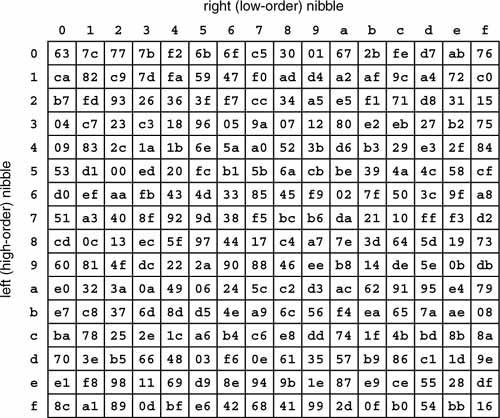
\includegraphics[height=10cm, width=10cm, keepaspectratio]{Immagini/Capitolo2/rijndael_sbox.png}}
	\caption{il 97-esimo byte è il numero 61 HEX in esadecimale, quindi è mappato nel byte nella riga 6 e colonna 1 che è EF HEX che corrisponde
al 239-esimo byte. In binario si ha che $(1100001)_{2} = (97)_{10}$
è mappato in $(11101111)_{2} = (239)_{10}$ \label{fig:Rij_mixcol}} 	
\end{figure}

\begin{figure}[htbp]
	\centering%
	\subfigure%
	{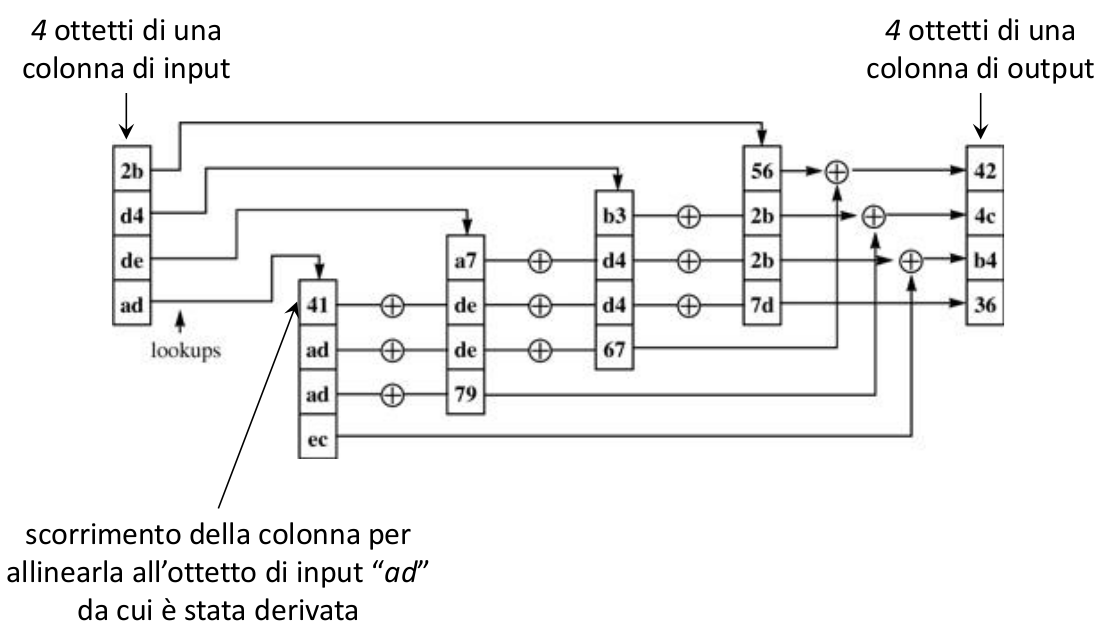
\includegraphics[height=13cm, width=13cm, keepaspectratio]{Immagini/Capitolo2/rijndael_mixcol.png}}
	\caption{MixColumn \label{fig:Rij_mixcol}} 	
\end{figure}

\begin{figure}[htbp]
	\centering%
	\subfigure%
	{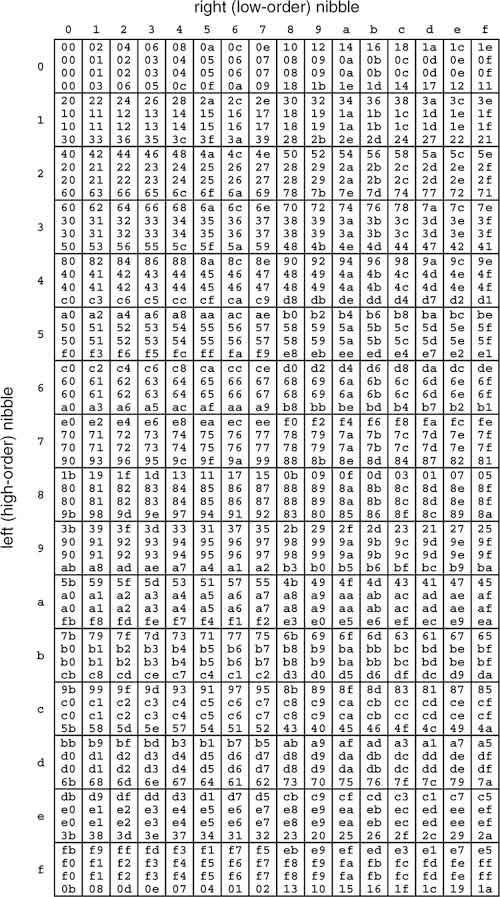
\includegraphics[height=13cm, width=13cm, keepaspectratio]{Immagini/Capitolo2/rijndael_mixcol_lookup.png}}
	\caption{All'ottetto "2b" corrisponde la colonna di 4 ottetti che si trova all’incrocio della riga "2" e della colonna "b", cioè la colonna ["56";"2b";"2b";"7d"] \label{fig:Rij_mixcol_lookup}} 	
\end{figure}

\subsubsection{Invertibilità delle operazioni primitive e decifratura di Rijndael}
\begin{itemize}
  \item L'or-esclusivo è chiaramente invertibile, come discusso nel capitolo dedicato a DES
  \item L'inversa della S-box si ottiene considerando semplicemente una tabella diversa (ovviamente la tabella inversa)
  \item L'inversa dello scorrimento circolare di una riga o colonna si ottiene semplicemente eseguendo lo stesso scorrimento, ma in direzione opposta
  \item L'inversa di MixColumn, detta InvMixColumn, è esattamente come MixColumn, ma con una tabella di lookup diversa
\end{itemize}

Il cifrario inverso di Rijndael può pertanto implementarsi applicando le inverse delle operazioni primitive, eseguite in sequenza opposta rispetto quella di cifratura. Tuttavia si può mostrare che, grazie alle proprietà matematiche di cui gode Rijndael, il cifrario inverso ha una struttura molto simile al cifrario diretto, ma con operazioni invertite, e con le chiavi di round non soltanto in ordine inverso, ma con InvMixColumn applicato a tutte tranne la prima e l'ultima colonna.

\subsubsection{Funzionamento di un Round}
Ogni round di Rijndael è costituito da una sequenza identica di tre operazioni::
\begin{enumerate}
  \item Ogni ottetto della matrice di stato viene sottoposto alla S-box
  \item Vengono effettuati una serie di scorrimenti circolari:
  		\begin{itemize}
  			\item la riga 1 dello stato viene fatta scorrere a sx di una colonna
  			\item la riga 2 dello stato viene fatta scorrere a sx di $2 + \lfloor \frac{N_{b}}{8} \rfloor$ colonne (2 se $N_{b} < 8$, 3 altrimenti)
  			\item la riga 3 dello stato viene fatta scorrere a sx di $3 + \lfloor \frac{N_{b}}{7} \rfloor$ colonne (3 se $N_{b} < 7$, 4 altrimenti)
		\end{itemize}
		(in AES si semplifica in scorrimento a sx di i colonne della riga i)
  \item Ogni colonna dello stato viene sottoposta alla MixColumn; il round $N_{r}$ omette questa operazione
\end{enumerate}

\subsubsection{Round invertito}
Essendo ogni operazione invertibile la decifratura può effettuarsi applicando in ordine inverso l'inversa (in senso matematico) di ogni operazione, e usando le chiavi di round in ordine inverso. Tuttavia la decifratura può avere la stessa struttura della cifratura: è necessario usare le chiavi di round in ordine opposto, e applicare InvMixColumn ad ogni colonna delle chiavi espanse tranne quelle del round iniziale e finale.

\section{Cifrari a flusso e RC4}
Sebbene i cifrari a blocchi siano molto più comuni, in alcune applicazioni i cifrari a flusso sono più adatti. Si pensi ad applicazioni che richiedono la cifratura/decifratura di un flusso di dati (come le trasmissioni di stream audio/video). Di seguito sarà esaminato il cifrario a flusso più popolare: \textbf{RC4} e  preliminarmente sarà discussa la struttura generale diun cifrario a flusso.

\subsection{Struttura di un cifrario a flusso}
\begin{figure}[htbp]
	\centering%
	\subfigure%
	{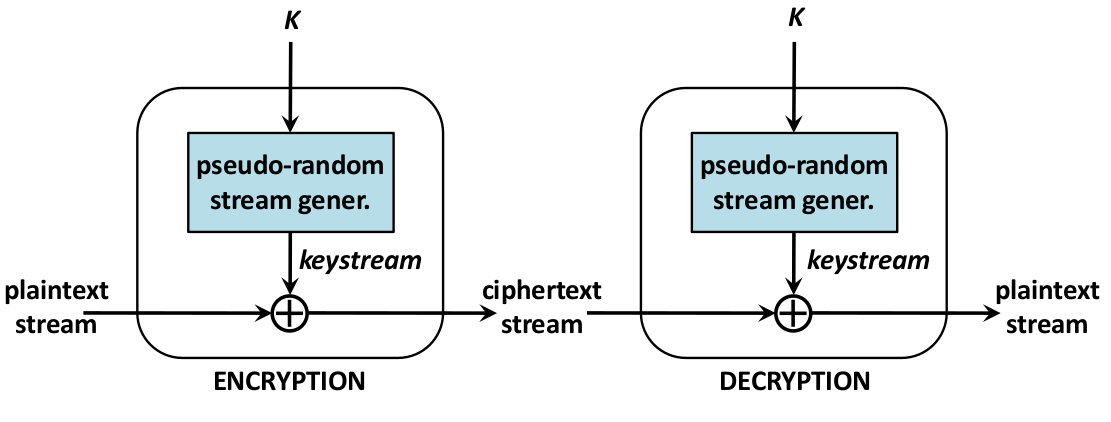
\includegraphics[height=13cm, width=13cm, keepaspectratio]{Immagini/Capitolo2/flusso_struct.png}}
	\caption{Struttura di un cifrario a flusso \label{fig:flusso_struct}} 	
\end{figure}

Un tipico cifrario a flusso cifra il testo in chiaro un byte per volta (sebbene possa essere progettato per agire su unità più grandi di un byte). La chiave segreta \textbf{K} (di lunghezza finita) è l'ingresso di un generatore \textbf{pseudo-casuale} di bit che produce un flusso (di lunghezza arbitraria) di byte apparentemente casuale, chiamato chiave di flusso (\textbf{keystream}). La chiave di flusso è un flusso "\textbf{impredicibile}" se non si conosce la chiave (nel senso che non presenta regolarità statistiche), ma viene generato in modo deterministico a partire dalla questa. \\

Il keystream è combinato un byte alla volta con il flusso del testo in chiaro mediante un or-esclusivo \textbf{bit a bit}, e il risultato di questo processo è il flusso cifrato. Ad esempio, se $p_{i} = 11001100$ è l'i-esimo byte del flusso del testo in chiaro, e $k_{i} = 01101100$ è l'i-esimo byte del keystream, allora l'i-esimo byte del flusso del testo cifrato è:

\begin{equation}
	c_{i} = p_{i} \oplus k_{i} = 10100000
\end{equation}

La decifratura richiede l'uso della stessa sequenza pseudo-casuale (keystream) combinata un byte alla volta con il testo cifrato mediante or-esclusivo \textbf{bit a bit}. Ad esempio, se $c_{i} = p_{i} \oplus k_{i} = 10100000$ è l’i-esimo byte del flusso del testo cifrato, e $k_{i} = 01101100$ è l'i-esimo byte del keystream, allora l'i-esimo byte del flusso del testo in chiaro è: 

\begin{equation}
	p_{i} = c_{i} \oplus k_{i} = (p_{i} \oplus k_{i}) \oplus k_{i} = p_{i} \oplus (k_{i} \oplus k_{i}) = p_{i} = 11001100
\end{equation}

Più è casuale l'aspetto del keystream, più è randomizzato il testo cifrato, rendendo la crittoanalisi più difficile. Pertanto il keystream dovrebbe avere un periodo grande (la funzione deterministica che genera il keystream, a partire dalla chiave segreta, è per forza di cose periodica), e dovrebbe approssimare il più possibile un flusso casuale. Ad esempio, 0 e 1 dovrebbero essere equamente presenti e riguardando il keystream come una sequenza di byte, tutti i 256 possibili byte dovrebbero apparire "disordinatamente" e con una frequenza uniforme. Come nei cifrari a blocchi, è necessario che la chiave sia sufficientemente lunga per proteggersi dagli attacchi a forza bruta (è preferibile una lunghezza della chiave di almeno 128 bit).

\subsection{Cifrari a flusso vs cifrari a blocchi}
\begin{figure}[htbp]
	\centering%
	\subfigure%
	{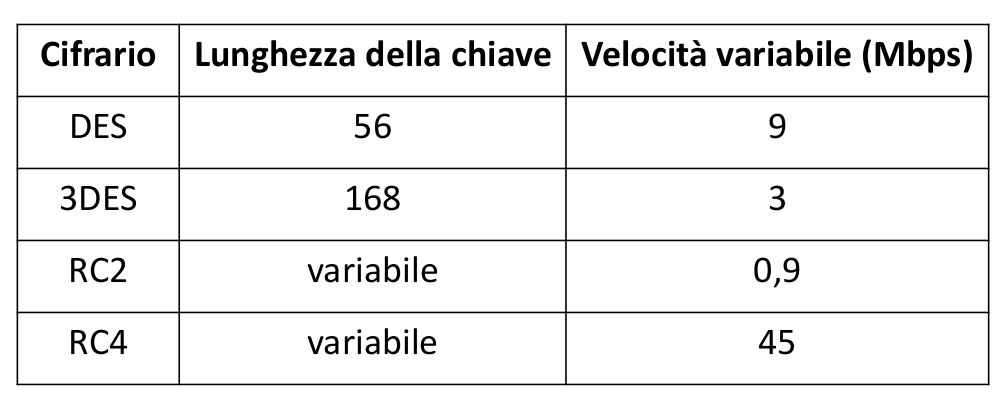
\includegraphics[height=13cm, width=13cm, keepaspectratio]{Immagini/Capitolo2/flusso_vel.png}}
	\caption{Confronto delle velocità di cifrari simmetrici su un Pentium II \label{fig:flusso_vel}} 	
\end{figure}
Se un cifrario a flusso è correttamente progettato, a parità di lunghezza della chiave segreta, può essere sicuro tanto quanto un cifrario a blocchi. Il vantaggio principale di un cifrario a flusso è che è quasi sempre più veloce (vedi \figurename ~\ref{fig:flusso_vel}), ed è facilmente implementabile.\\

Il vantaggio di un cifrario a blocchi è che la chiave segreta è riutilizzabile per più comunicazioni, mentre nei cifrari a flusso è sconsigliato. Infatti, se due testi in chiaro sono cifrati con la stessa chiave segreta, usando un cifrario a flusso, la crittoanalisi è spesso molto semplice: basta sommare XOR i due flussi di testo cifrato per ottenere la somma XOR dei due testi in chiaro. Se i testi in chiaro sono stringhe testuali, numeri di carta di credito o altri flussi di byte con proprietà note la crittoanalisi può aver successo.

\subsection{RC4}
RC4 è un cifrario a flusso progettato nel 1987 da Ron Rivest (RSA Security) con dimensione della chiave variabile e funzionamento orientato al byte. Si basa sull'uso di una permutazione casuale, e dagli studi svolti sembra che il periodo del cifrario sia superire a $10^{100}$. Viene usato negli standard \textbf{SSL/TLS} (\textit{Secure Socket Layer/Transport Layer Security}), nel protocollo \textbf{WEP} (\textit{Wired Equivalent Privacy}) e nel protocollo \textbf{WPA} (\textit{WiFi Protected Access}). L'algoritmo RC4 è molto semplice da spiegare: basta capire come viene generato il
\textbf{keystream}. \\

L’algoritmo mantiene un array di stato monodimensionale \textbf{S} contenente 256 byte. S[0], S[1], ..., S[255] sono i 256 byte, ciascuno dei quali rappresenta un numero da 1 a 255. Una chiave di lunghezza variabile da 1 a 256 byte (da 8 a 2048 bit) viene usata per inizializzare il contenuto dell'array di stato. Quindi \textbf{S} contiene, in ogni momento, una delle 256! permutazioni dei numeri da 0 a 255. Per la cifratura/decifratura viene generato un byte \textbf{k} selezionando da \textbf{S} uno dei 255 elementi in maniera sistematica. Subito dopo la generazione del byte \textbf{k}, gli elementi di \textbf{S} vengono permutati, e l'algoritmo prosegue alternando le ultime due fasi (generazione di k e permutazione) finché il flusso in input non termina.\\

\subsubsection{Inizializzazione}
Gli elementi di \textbf{S} vengono impostati uguali ai valori da 0 a 255 in ordine crescente:
\begin{equation}
	S[0] = 0, S[1] = 1, ..., S[255] = 255
\end{equation}
Un vettore temporaneo \textbf{T}, della stessa lunghezza di \textbf{S}, viene usato per memorizzare temporaneamente la chiave \textbf{K}. Se la lunghezza di \textbf{K} è 256 byte \textbf{K} viene trasferita in \textbf{T}. Altrimenti, \textbf{K} viene copiata più volte in \textbf{T} fino a riempirlo.

\begin{algorithm}
\begin{lstlisting}[caption={Inizializzazione RC4}]
for i = 0 to 255 do {
	S[i] = i;
	T[i] = K[i mod keylen]; // keylen: lunghezza di S
}
\end{lstlisting}
\end{algorithm}

\subsubsection{Permutazione iniziale}
successivamente si userà T per produrre la \textit{permutazione iniziale}. Si scandisce \textbf{S} e per ciascun S[i], si scambia S[i] con un altro elemento di S scelto in modo sistematico in base, tra l'altro, al contenuto di T[i]. Poiché la sola operazione su \textbf{S} è lo scambio, il solo effetto è una permutazione (\textbf{S} contiene ancora tutti i numeri da 0 a 255).

\begin{algorithm}
\begin{lstlisting}[caption={Permutazione iniziale RC4}]
j = 0;
for i = 0 to 255 do {
	j = (j + S[i] + T[i]) mod 256;
	scambia(S[i], S[j]);
}
\end{lstlisting}
\end{algorithm}

\subsubsection{Generazione del flusso}
Una volta che \textbf{S} è inizializzato, la chiave segreta \textbf{K} (quindi anche l'array \textbf{T}) non viene più utilizzata. Il keystream viene generato facendo una
scansione ciclica di \textbf{S}. Ciascun elemento S[i] viene scambiato con un altro byte di \textbf{S} a secondo di uno schema che dipende dalla configurazione corrente di \textbf{S}, dopodiché viene generato un singolo byte \textbf{k} del keystream sempre in base alla configurazione corrente di \textbf{S}.

\begin{algorithm}
\begin{lstlisting}[caption={Generazione flusso}]
i, j = 0;
while (true) {
	i = (i + 1) mod 256;
	j = (j + S[i]) mod 256;
	scambia(S[i], S[j]);
	t = (S[i] + S[j]) mod 256;
	k = S[t];
}
\end{lstlisting}
\end{algorithm} 
\chapter{Modes of Operation}

\section{Introduzione}
Si illustrerà come usare gli algoritmi di crittografia a chiave segreta, DES, IDEA e AES, in applicazioni reali: è stato visto soltanto come usare tali algoritmi per cifrare blocchi di lunghezza prefissata (64 bit per DES e IDEA, 128 bit per AES), come si procede se è necessario cifrare dei messaggi di lunghezza arbitraria/diversa? \newline \newline
Si vedrà inoltre come si generano dei MAC (\textbf{M}essage \textbf{A}uthentication \textbf{C}ode) sfruttando la crittografia a chiave segreta.

\section{Cifrare messaggi di grandi dimensioni}
Come è possibile cifrare messaggi di dimensioni superiori a 64 bit? \newline
Sono state proposte diverse \textbf{modalità operative dei cifrari a blocchi}, cioè ci si è interrogati su come utilizzare i cifrari a blocchi nel caso di messaggi di lunghezza maggiore di quella di un singolo blocco.\newline \newline
Le modalità più conosciute e che verranno descritte di seguito sono:
\begin{itemize}
  \item \textbf{E}lectronic \textbf{C}ode \textbf{B}ook (ECB)
  \item \textbf{C}ipher \textbf{B}lock \textbf{C}haining (CBC)
  \item k-Bit \textbf{C}ipher \textbf{F}eed\textbf{B}ack Mode (CFB)
  \item k-Bit \textbf{O}utput \textbf{F}eed\textbf{B}ack Mode (OFB)
  \item \textbf{C}oun\textbf{T}e\textbf{R} Mode (CTR)
\end{itemize} 
Si noti che nel seguito si farà riferimento a cifrari a blocchi con blocchi di 64 bit (tutte le considerazioni valgono anche nel casi di cifrari con blocchi di dimensione diversa da 64 bit).
\subsection{Electronic Code Book (ECB)}
Questa modalità consiste nel fare la cosa più ovvia, ma corrisponde, in genere, alla soluzione peggiore, cioè:
\begin{itemize}
\item il messaggio viene decomposto in blocchi da 64 bit (inserendo eventualmente dei bit di padding nell'ultimo blocco al fine di riempirlo)
\item ciascun blocco da 64 bit viene cifrato con la chiave segreta
\item ciascun blocco cifrato viene decifrato
\item il messaggio viene ricomposto a partire dai singoli blocchi decifrati
\end{itemize}
Come illustrato nella figure \figurename ~\ref{fig:ECB_enc} e \figurename ~\ref{fig:ECB_dec}
\begin{figure}[htbp]
	\centering%
	\subfigure%
	{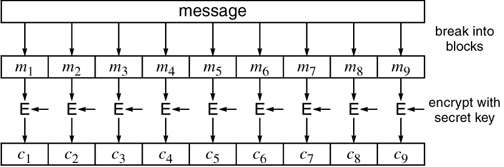
\includegraphics[height=4cm, width=12cm, keepaspectratio]{Immagini/Capitolo3/ECB_enc.png}}
	\caption{Schema di crittografia ECB \label{fig:ECB_enc}} 	
	\subfigure%
	{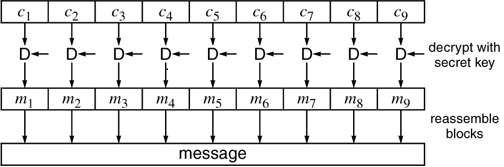
\includegraphics[height=4cm, width=12cm, keepaspectratio]{Immagini/Capitolo3/ECB_dec.png}}
	\caption{Schema di decrittografia ECB \label{fig:ECB_dec}} 
\end{figure}
\subsubsection{Problemi di sicurezza in ECB}
La modalità operativa ECB introduce una serie di problemi non presenti nel cifrario a blocchi: se il messaggio contiene due blocchi di 64 bit identici, allora anche i corrispondenti blocchi cifrati saranno identici e ciò fornisce delle informazioni aggiuntive sul testo in chiaro che un ascoltatore può sfruttare.
\begin{figure}
\centering%
	\subfigure%
	{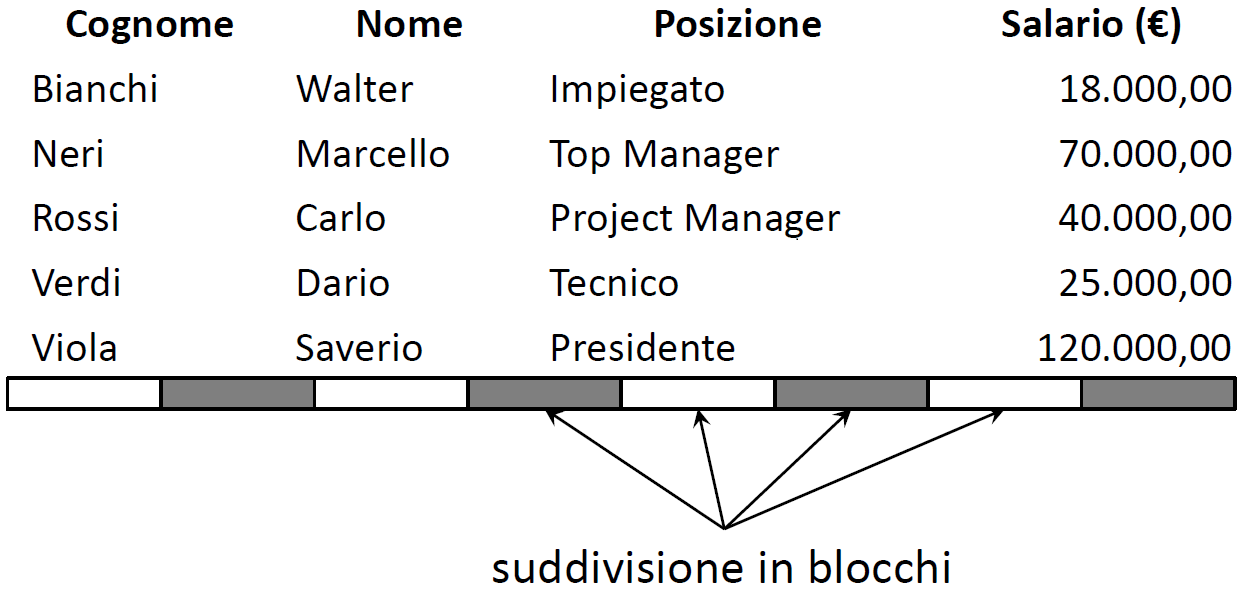
\includegraphics[height=6cm, width=10cm, keepaspectratio]{Immagini/Capitolo3/File_salari.png}}
	\caption{File con i salari, oggetto di attacco \label{fig:File_salari}} 	
\end{figure}
Si consideri ad esempio lo scenario della \figurename ~\ref{fig:File_salari}: supponiamo che l'ascoltatore sappia che il testo in chiaro contiene l'elenco, ordinato alfabeticamente, degli impiegati e dei relativi salari inviato dall'amministrazione all'ufficio paghe, supponiamo inoltre che ogni riga del file sia lunga esattamente 64 byte (8 blocchi da 8 byte) e che i vari blocchi risultino suddivisi in modo tale che alcuni contengono la codifica della cifra decimale più significativa del campo salario (migliaia di dollari/euro). Comparando i testi cifrati, l'ascoltatore, oltre a dedurre quanti dipendenti hanno lo stesso salario, può anche dedurre quanti dipendenti hanno uno stipendio nello stesso range (ordine di 10 euro/dollari); se ci sono complessivamente pochi range salariali, l'ascoltatore può dedurre a quale categoria di dipendente corrisponda un dato blocco cifrato; inoltre, se l'ascoltatore è un impiegato, può sostituire il blocco cifrato di un altro dipendente (un manager) al suo blocco cifrato (dedotto in base all'ordine e alla
numerosità della sua classe salariale).\newline \newline
ECB quindi ha due serie debolezze, legate al fatto che qualcuno, analizzando diversi blocchi cifrati potrebbe:
\begin{itemize}
\item dedurre (inferire) informazioni sfruttando le ripetizioni di alcuni blocchi
\item riarrangiare/modificare i blocchi cifrati a proprio vantaggio
\end{itemize}
Per tali ragioni ECB è raramente usato.
\subsection{Cipher Block Chaining (CBC)}
CBC non presenta i problemi di ECB: a due blocchi in chiaro identici non corrispondono
due blocchi cifrati identici.
\subsubsection{Idea base}
Per comprendere CBC conviene prima considerare il seguente esempio, in riferimento alla \figurename ~\ref{fig:rand_ele_cb_enc} che ne condivide l’idea base:
\begin{itemize}
\item per ogni blocco di testo in chiaro mi viene generato un numero random a 64 bit $r_{i}$
\item $m_{i}$ e $r_{i}$ vengono sommati ($\oplus$ XOR)
\item il risultato viene cifrato con la chiave segreta
\item i blocchi cifrati $c_{i}$ e i numeri random, in chiaro, $r_{i}$ vengono trasmessi
\end{itemize}
E per riottenere il testo in chiaro:
\begin{itemize}
\item vengono decifrati i blocchi $c_{i}$ con la chiave segreta 
\item i blocchi risultanti vengono sommati ($\oplus$ XOR) con i numeri random $r_{i}$
\end{itemize}
\begin{figure}
\centering%
	\subfigure%
	{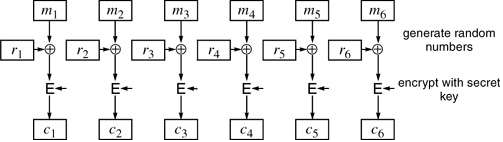
\includegraphics[height=5cm, width=10cm, keepaspectratio]{Immagini/Capitolo3/rand_ele_cb_enc.png}}
	\caption{Randomized Electronic Code Book Encryption\label{fig:rand_ele_cb_enc}} 	
\end{figure}
L'esempio appena visto è molto inefficiente, infatti l'informazione da trasmettere è duplicata perché per ogni blocco va trasmesso il corrispondente numero random. \newline
Un altro problema è che un avversario può riarrangiare i blocchi in modo da ottenere un effetto predittivo sul testo in chiaro, ad esempio:
\begin{itemize}
\item se la coppia $r_{2}|c_{2}$ fosse rimossa il corrispondente blocco in chiaro $m_{2}$ scomparirebbe 
\item se la coppia $r_{2}|c_{2}$ fosse scambiata con la coppia $r_{7}|c_{7} \Rightarrow$ $m_{2}$ e $m_{7}$ risulterebbero scambiati
\item se l’avversario conosce ciascun  $m_{i}$, può modificare  $m_{i}$ in modo predittivo cambiando il corrispondente numero random $r_{i}$
\end{itemize}
\subsubsection{Funzionamento}
CBC genera i “propri” numeri random usando $c_{i}$ come numero random $r_{i+1}$, cioè usa il precedente blocco cifrato come numero random da sommare ($\oplus$ XOR) al blocco di testo in chiaro successivo.\newline
Per evitare che due testi in chiaro inizialmente identici diano luogo a dei blocchi cifrati inizialmente identici CBC genera un singolo numero random, detto vettore di inizializzazione (\textbf{Initialization Vector $IV$}), che viene sommato ($\oplus$ XOR) con il primo blocco di testo in chiaro. \newline
Il risultato viene trasmesso dopo la cifratura a chiave segreta. \newline
La decifratura è semplice essendo l'or-esclusivo un'operazione che coincide con la propria inversa.\newline
Quanto detto, rappresentato nelle figure \figurename ~\ref{fig:CBC_enc} e \figurename ~\ref{fig:CBC_dec}, può essere espresso anche algebricamente:
\begin{itemize}
\item CIFRATURA\newline $c_{1} = E(K, (IV \oplus m_{1}))$\newline $c_{i} = E(K, (c_{i-1} \oplus m_{i})) \forall i > 1$
\item DECIFRATURA\newline $m_{1} = E(K,c_{1})\oplus IV$\newline $m_{i} = E(K,c_{i})\oplus c_{i-1}$
\end{itemize}
\begin{figure}[htbp]
	\centering%
	\subfigure%
	{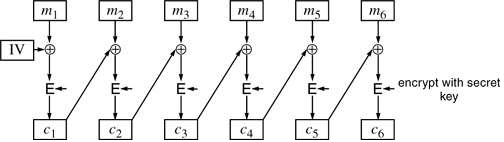
\includegraphics[height=4cm, width=12cm, keepaspectratio]{Immagini/Capitolo3/CBC_enc.png}}
	\caption{Schema di crittografia CBC \label{fig:CBC_enc}} 	
	\subfigure%
	{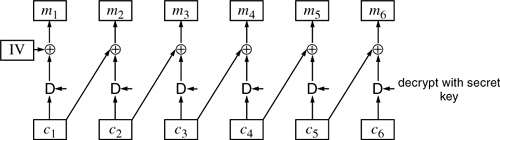
\includegraphics[height=4cm, width=12cm, keepaspectratio]{Immagini/Capitolo3/CBC_dec.png}}
	\caption{Schema di decrittografia CBC \label{fig:CBC_dec}} 
\end{figure}
Si noti che, essendo il costo della somma ($\oplus$ XOR) trascurabile rispetto al costo della cifratura a chiave segreta, la cifratura con CBC ha le stesse prestazioni della cifratura con ECB eccetto il costo delle generazione e trasmissione di $IV$. In molti casi, tuttavia, la sicurezza di CBC non dipende dalla
scelta del vettore di inizializzazione $IV$ (cioè si possono anche porre tutte le cifre di $IV$ pari a 0).\newline \newline
In alcuni casi, tuttavia, l'assenza di $IV$ riduce la sicurezza. Ad esempio, si supponga che il file cifrato contenente i salari dei dipendenti sia trasmesso settimanalmente; in assenza di $IV$, un ascoltatore potrebbe verificare se il testo cifrato differisce da quelle della precedente settimana, e potrebbe determinare la prima persona il cui salario è cambiato. Un altro esempio è quello di un generale che invia
giornalmente delle informazioni segrete dicendo “continue holding your position”; il testo cifrato sarebbe ogni giorno lo stesso, finché il generale decide di cambiare ordine, inviando il messaggio “start bombing”: il testo cifrato cambierebbe immediatamente, allertando il nemico.\newline
Un vettore di inizializzazione scelto randomicamente garantisce che, anche se lo stesso messaggio è inviato ripetutamente, il corrispondente testo cifrato risulta ogni volta differente, e previene attacchi all'algoritmo di cifratura di tipo testo in chiaro selezionato anche quando un avversario può fornire del testo in chiaro al CBC.
\subsubsection{CBC minaccia 1 – Modifica dei blocchi cifrati}
L’uso di CBC non elimina il problema che qualcuno possa modificare il messaggio in transito, semplicemente cambia la natura della minaccia: un avversario non può più vedere ripetizioni di blocchi cifrati, e non può più copiare/spostare blocchi cifrati (ad esempio per scambiare il salario di due dipendenti) ma può ancora modificare il testo cifrato in modo predittivo. \newline
Cosa potrebbe succedere se modificasse un blocco di testo cifrato, ad esempio $c_{n}$?\newline
Da $m_{n+1} = E(K,c_{n+1})\oplus c_{n}$ si evince che una modifica di $c_{n}$ può avere un effetto prevedibile su $m_{n+1}$ (ad esempio, cambiando il terzo bit di $c_{n}$ cambia il terzo bit di $m_{n+1}$);
chiaramente essendo anche $m_{n} = E(K,c_{n})\oplus c_{n-1}$,  l'avversario non può prevedere quale possa essere il nuovo valore di $m_{n}$, molto probabilmente la modifica di $c_{n}$ corrompe completamente il blocco in chiaro $m_{n}$.\newline
Vediamo a tal proposito l'esempio seguente, illustrato in \figurename ~\ref{fig:modifica_blk_cifrati}:
\begin{figure}[htbp]
	\centering%
	\subfigure%
	{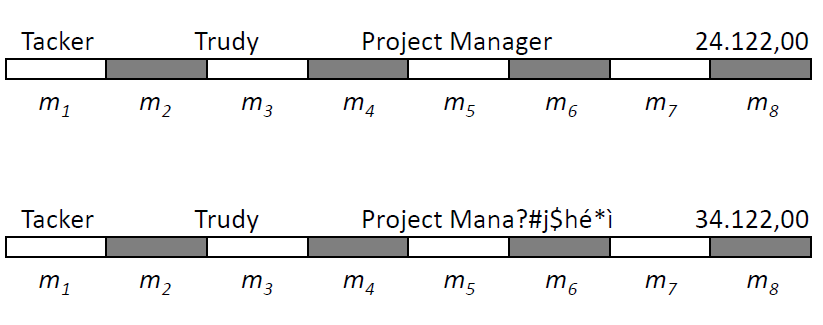
\includegraphics[height=4cm, width=12cm, keepaspectratio]{Immagini/Capitolo3/modifica_blk_cifrati.png}}
	\caption{Modifica dei blocchi cifrati \label{fig:modifica_blk_cifrati}}	
\end{figure}
\newline Supponiamo che un avversario (Trudy) sappia che una data sequenza di blocchi cifrati, del file
dei salari, corrispondano alla riga contenente i suoi dati personali; se Trudy vuole aumentare il suo salario di 10K, e se sa che l'ultimo byte di $m_{7}$ corrisponde alle decine di migliaia nella codifica decimale (00000010), per darsi 10K in più deve semplicemente cambiare il bit meno significativo di $c_{6}$; da $m_{7} = D(K, c_{7}) \oplus c_{6}$ tuttavia, Trudy non sarà più in grado di predire cosa apparirà nella voce “Posizione”, infatti, da $m_{6} = D(K, c_{6}) \oplus c_{5}$, si vede che è impraticabile
prevedere l'effetto della modifica di $c_{6}$ su $m_{6}$. Se il file decifrato fosse letto da una persona umana, questa potrebbe insospettirsi della presenza di simboli strani nel campo “Posizione”, se invece il file decifrato viene elaborato da un programma l'attacco potrebbe non essere rilevato.\newline \newline
Ricapitolando: Trudy è stato in grado di modificare un blocco in modo predittivo con l'effetto collaterale di modificare il blocco precedente senza poter prevedere il risultato finale.
\subsubsection{CBC minaccia 2 – Riarrangiamento blocchi cifrati}
Con riferimento alla \figurename ~\ref{fig:riarrangiamento_blk_cifrati}, si supponga che Trudy conosca il testo in chiaro e, il corrispondente testo cifrato di qualche messaggio, cioè $m_{1}$, $m_{2}$, ..., $m_{n}$ e $IV$, $c_{1}$, $c_{2}$, ..., $c_{n}$; in questo modo Trudy conosce automaticamente anche il blocco decifrato di ciascun $c_{i}$, da $D(K, c_{1}) = c_{i-1} \oplus m_{i}$.
\begin{figure}[htbp]
	\centering%
	\subfigure%
	{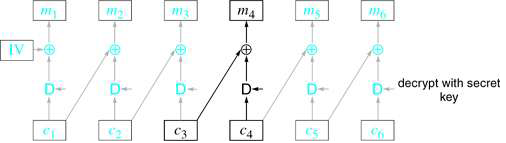
\includegraphics[height=3cm, width=12cm, keepaspectratio]{Immagini/Capitolo3/riarrangiamento_blk_cifrati.png}}
	\caption{Riarrangiamento dei blocchi cifrati \label{fig:riarrangiamento_blk_cifrati}}	
\end{figure}
Da queste informazioni, Trudy può considerare ciascun $c_{i}$ come un "building block" e costruire un flusso cifrato usando ogni combinazione di $c_{i}$ ed essere in grado di calcolare quale sarà il corrispondente testo in chiaro. \newline \newline
Per capire a cosa potrebbe servire questo tipo di attacco si tenga presente che uno dei modi di combattere la minaccia di modifica di blocchi cifrati è includere un \textbf{CRC} (\textbf{C}yclic \textbf{R}edundancy \textbf{C}heck) al testo in chiaro prima di cifrarlo con un CBC, perciò se Trudy modifica qualche blocco cifrato, il CRC consentirà ad un computer di rilevare prontamente l'alterazione del messaggio (e.g. se si fosse scelto un CRC a 32 bit ci sarebbe una possibilità su $2^32$ che il CRC coincida con quello corretto); supponiamo che a Trudy non interessi quale possa essere il nuovo messaggio di testo in chiaro (che potrebbe essere completamente indecifrabile), ma interessi solamente che il nuovo messaggio manomesso sia accettato dal computer ricevente sapendo che viene eseguito un controllo di tipo CRC, Trudy può provare a costruire molti flussi cifrati combinando in modi diversi i blocchi $c_{1}$, $c_{2}$, ..., $c_{n}$ e può calcolare il risultante testo in chiaro per ciascuno di essi, per poi testare se il testo in chiaro risultante ha un CRC corretto (mediamente serviranno $2^31$ tentativi).\newline 
Che male potrebbe fare Trudy modificando un messaggio, senza controllarne il contenuto, in modo
tale che sia accettato dal computer ricevente? Forse Trudy è soltanto maliziosa, e vuole distruggere
alcuni dati che vengono caricati attraverso la rete, ma in realtà, c'è un modo sottile di controllare, seppur in misura ridotta, il contenuto del messaggio modificato: supponiamo che Trudy sposti blocchi contigui, ad esempio, se $c_{n}$ e $c_{n+1}$ vengono spostati in qualche altro posto, allora il blocco originale $m_{n+1}$ apparirà in un'altra posizione; se $m_{n+1}$ contiene il salario del presidente, Trudy
potrebbe scambiare i blocchi in modo da cambiarlo con il suo, ma poi dovrà modificare molto probabilmente gran parte del messaggio restante per garantire che il CRC risulti invariato.\newline \newline
Per prevenire attacchi di questo tipo, basati sul riarrangiamento dei blocchi cifrati e tali da preservare il CRC originario, potrebbe essere usato un CRC a 64 bit: ciò è sicuramente sufficiente se l'attacco al CRC, nell'ambito di un CBC, è di tipo a forza bruta. \newline
Per chi progetta protocolli crittografici sicuri, una modalità di cifratura ad un singolo step che protegga sia la confidenzialità che l'autenticità di un messaggio è stata per molti anni una sorta di "Sacro Graal" da ricercare!
\subsection{Output FeedBack Mode (OFB)}
L’OFB è un cifrario a flusso: la cifratura consiste nel sommare ($\oplus$ XOR) il messaggio con il keystream (o one-time pad) generato da OFB stesso. Supponiamo che il keystream sia ottenuto generando singoli blocchi di 64 bit alla volta; un possibile modo per generarlo è il seguente:
\begin{itemize}
\item viene generato un numero random $IV$ (Initialization Vector) di 64 bit
\item il primo blocco del keystream coincide con $IV$: $b_{0} = IV$
\item i blocchi seguenti $b_{i}$ si ottengono cifrando $b_{i-1}$ con la chiave segreta: $b_{i} = E(K,b_{i-1})$
\end{itemize}
Il one-time pad (keystream) risultante è dato dalla sequenza $OTP = OTP(K, IV) = b_{0}|b_{1}|b_{2}|…|b_{i}|b_{i+1}|…$.
La cifratura con OFB (\figurename ~\ref{fig:OFB_enc}) consiste nel sommare ($\oplus$ XOR) il messaggio $m$ con OTP, se $m$ ha lunghezza $l_{m}$ bit si considereranno soltanto $l_{m}$ bit di OTP.
\begin{figure}[htbp]
	\centering%
	\subfigure%
	{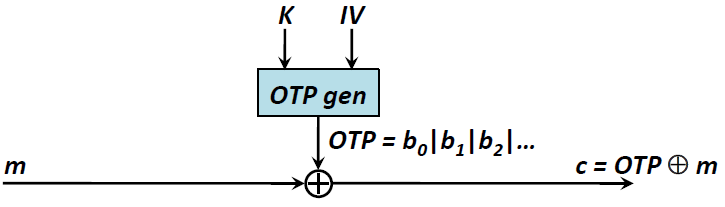
\includegraphics[height=4cm, width=12cm, keepaspectratio]{Immagini/Capitolo3/OFB_enc.png}}
	\caption{Schema di crittografia OFB \label{fig:OFB_enc}} 	
\end{figure}
Il risultato della cifratura $c = OTP \oplus m$ viene trasmesso insieme a $IV$ (la lunghezza $l_{c}$ di c coincide con $l_{m}$).\newline
In decifratura (\figurename ~\ref{fig:OFB_dec}) il destinatario riceve $IV$ e conoscendo $K$ calcola lo stesso onetime pad $OTP = OTP(K, IV)$  il messaggio $m$ si ottiene sommando ($\oplus$ XOR) il flusso cifrato $c$ con $l_{c}$ bit di OTP.
\begin{figure}[htbp]
	\centering%
	\subfigure%
	{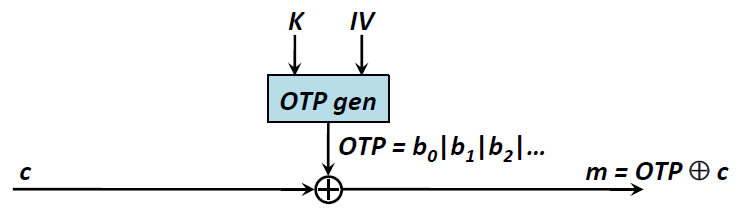
\includegraphics[height=4cm, width=12cm, keepaspectratio]{Immagini/Capitolo3/OFB_dec.png}}
	\caption{Schema di decrittografia OFB \label{fig:OFB_dec}} 	
\end{figure}
\subsubsection{Vantaggi e svantaggi di OFB}
OFB presenta i seguenti vantaggi:
\begin{itemize}
\item visto che il one-time pad OTP può essere generato in anticipo, prima che sia noto il messaggio m da cifrare, una volta ottenuto m è necessario soltanto effettuare la somma ($\oplus$ XOR) con il one-time pad (lo XOR è eseguibile in modo estremamente veloce)
\item se qualche bit del testo cifrato dovesse corrompersi, soltanto i corrispondenti bit del testo in chiaro sarebbero corrotti, diversamente dalla modalità CBC, dove se $c_{n}$ fosse corrotto allora $m_{n}$ sarebbe completamente corrotto e $m_{n+1}$ sarebbe corrotto in corrispondenza dei medesimi bit di $c_{n}$
\item un messaggio m può arrivare a pezzi di lunghezza arbitraria, e, ogni volta che arriva un pezzo, il corrispondente testo cifrato può essere immediatamente trasmesso; in CBC invece, se il messaggio arriva un byte alla volta, per la cifratura è comunque necessario attendere che un blocco di 64 bit (o un multiplo intero di 8 byte) sia completo (ciò può comportare l'attesa di altri 7 byte o l'aggiunta di bit di riempimento, cosa che aumenta la quantità di dati da trasmettere)
\end{itemize}
OTP ha però anche il seguente svantaggio:
\begin{itemize}
\item se un avversario conoscesse il testo in chiaro m e quello cifrato c, potrebbe modificare il testo in
chiaro a piacimento semplicemente sommando il testo cifrato con il testo in chiaro noto, e sommando il risultato con un qualsiasi messaggio $m'$ che desidera sostituire ad m; cioè l'avversario dovrebbe modificare il testo cifrato come $c' = c \oplus m \oplus m'$ e verificare che decifrando $c'$ anziché $c$ si ottiene $m'$ anziché $m$.
\end{itemize}
\subsection{k-bit Output FeedBack Mode (k-OFB)}
In generale la modalità OFB consente di generare flussi di "pezzi" da $k$ bit (quanto visto prima corrisponde al caso in cui $k$ = 64 bit).
La modalità k-bit OFB funziona nel seguente modo (si descriverà la versione data in [DES81]) con riferimento alla \figurename ~\ref{fig:k-bit_OFB}:
\begin{figure}[htbp]
	\centering%
	\subfigure%
	{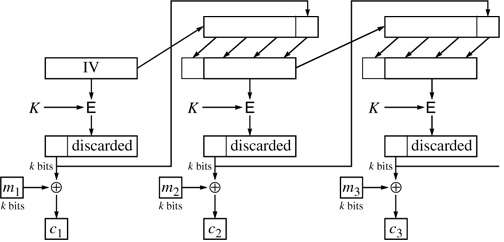
\includegraphics[height=4cm, width=12cm, keepaspectratio]{Immagini/Capitolo3/k-bit_OFB.png}}
	\caption{k-bit OFB \label{fig:k-bit_OFB}} 	
\end{figure}
\begin{itemize}
\item l'input $I_{0}$ al modulo di cifratura DES è inizializzato a $IV$, cioè $I_{0}=IV$: se $IV$ ha meno di 64 bit, vengono inseriti degli 0 di riempimento a sinistra (cifre più significative)
\item il primo pezzo $b_{0}$ di OTP si ottiene selezionando $k$ bit dall’output $O_{0} = E(K, I_{0})$ di DES (una quantità a 64 bit); da un punto di vista crittografico non ha importanza come siano scelti tali bit da $O_{0}$; [DES81] specifica che devono essere i $k$ bit più significativi
\item l’i-esimo pezzo $b_{i}$ si ottiene selezionando i $k$ bit più significativi dell'output $O_{i} = E(K, I_{i})$ di DES, ove l'input $I_{i}$ è stato ottenuto da $I_{i-1}$ eseguendo una traslazione a sinistra di $k$ bit, e un inserimento di $b_{i-1}$ nei $k$ bit meno significativi di $I_{1}$ ($k$ bit più a destra)
\end{itemize}
\subsection{Cipher FeedBack Mode (CFB)}
La modalità CFB è molto simile a OFB, con riferimento alla \figurename ~\ref{fig:k-bit_CFB}:
\begin{figure}[htbp]
	\centering%
	\subfigure%
	{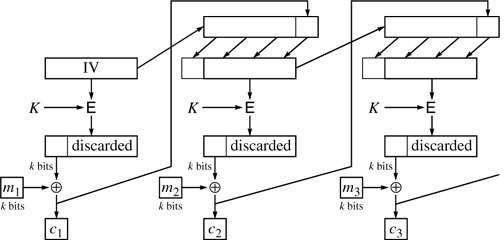
\includegraphics[height=4cm, width=12cm, keepaspectratio]{Immagini/Capitolo3/k-bit_CFB.png}}
	\caption{k-bit CFB \label{fig:k-bit_CFB}} 	
\end{figure}
\begin{itemize}
\item viene prodotto un one-time pad generando, uno alla volta, singoli pezzi di $k$ bit
\item il one-time pad viene sommato ($\oplus$ XOR) con pezzi di $k$ bit del messaggio
\end{itemize}
Si noti che in OFB i $k$ bit meno significativi dell'input $I_{i}$ del modulo di cifratura DES sono i $k$ bit di $b_{i-1}$ (sono parte dell'output $O_{i-1}$ della cifratura DES del blocco precedente; invece, in CFB i $k$ bit di $I_{i}$ sono i $k$ bit di testo cifrato del blocco precedente, cioè i $k$ bit di $c_{i-1}$ (in CFB il one-time pad non può essere generato prima che il messaggio e noto, a differenza di OFB), nella modalità a k-bit è ragionevole assegnare a $k$ un valore diverso da 64 bit (una scelta sensata è $k$ = 8 bit).
\subsubsection{Vantaggi e svantaggi  di CFB}
CBF presenta i seguenti vantaggi:
\begin{itemize}
\item Con OFB o CBC, se si ha una perdita di caratteri in trasmissione (testo cifrato), i.e. se nel flusso cifrato $c_{1}, c_{2}, c_{3}, ... , c_{n}, ...$ si perde il carattere $c_{k}$, allora a destinazione si ottiene la sequenza $c_{1}, c_{2}, c_{3}, ... , c_{k'}, ... , c_{n-1'}$ ove $c_{k'} = c_{k+1}, c_{k+1'} = c_{k+2}, ... , c_{k+i'} = c_{k+i+1}$; oppure, con OFB o CBC, se extra caratteri sono aggiunti al flusso cifrato, i.e. se nel flusso cifrato$c_{1}, c_{2}, c_{3}, ... , c_{n}, ...$ si aggiunge il carattere $c*$ dopo di $c_{k-1}$, allora a destinazione si ottiene la sequenza $c_{1}, c_{2}, c_{3}, ... , c_{k'}, ... , c_{n+1'}$ ove $c_{k'} = c*, c_{k+1'} = c_{k}, ... , c_{k+i'} = c_{k+i-1}$. Quindi l'intera parte restante della trasmissione risulta indecifrabile poiché $m_{i’} = c_{i’} \oplus b_{i}$ e $b_{i} = b_{i}(K, IV)$ cioè bi non dipende dalla sequenza cifrata. Invece, con 8-bit CFB, si ha un effetto risincronizzante: se un byte ci è perso in trasmissione allora corrispondente testo in chiaro mi è perso, e i successivi 8 byte $m_{i+1}, …, m_{i+8}$ risulteranno indecifrabili, ma dal byte $m_{i+9}$ in poi il testo in chiaro sarà corretto, questo perché $b_{i} = b_{i}(K, c_{i-1})$, cioè $b_{i}$ è derivato dalla sequenza di caratteri cifrati. Discorsi analoghi valgono nel caso dell'aggiunta di un byte al flusso cifrato.
\item i messaggi cifrati con CFB offrono più protezione di CBC e di OFB rispetto ad eventuali manomissioni; infatti, nel caso di 8-bit CFB un avversario può modificare ogni singolo byte in modo predittivo, ma con l'effetto collaterale di non poter prevedere/controllare i successivi 8 byte discorsi simili valgono per 64-bit CFB.
\item a differenza di CBC, non sono possibili attacchi basati sul riarrangiamento di blocchi; tuttavia intere sezioni del messaggio possono essere riarrangiate rendendo indecifrabili le parti corrispondenti ai "punti di giuntura".
\end{itemize}
CBF ha anche i seguenti svantaggi:
\begin{itemize}
\item 8-bit CFB ha lo svantaggio che ogni byte di input richiede un'operazione DES. Inizialmente CFB fu concepito per essere utilizzato con un numero arbitrario $k$ di bit per "pezzo", con $k$ minore della dimensione di un blocco completo (64 bit per DES); nella pratica tuttavia $k$ è pari a 1 byte oppure coincide con la dimensione piena (full-block) dei blocchi del modulo di cifratura. Quando utilizzato in modalità full-block le prestazioni di CFB sono comparabili a quelle di ECB, CBC, e OFB.
\item come OFB consente di cifrare ed inviare ciascun byte del messaggio non appena è noto tuttavia, a differenza di OFB non è in grado di anticipare il calcolo del one-time pad in fine, è in grado di rilevare delle alterazioni meglio di OFB, ma non bene quanto CBC.
\end{itemize}
\subsection{CounTeR Mode (CTR)}
CTR (\figurename ~\ref{fig:CTR}) è simile a OFB perché un one-time pad viene generato e sommato ($\oplus$ XOR) con i dati; tuttavia differisce da OFB perché non concatena ciascun blocco di one-time-pad con il precedente, ma incrementa $IV$ e poi cifra quanto ottenuto per ottenere il prossimo blocco di one-time pad. 
\begin{figure}[htbp]
	\centering%
	\subfigure%
	{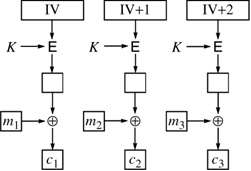
\includegraphics[height=4cm, width=12cm, keepaspectratio]{Immagini/Capitolo3/CTR.png}}
	\caption{CTR \label{fig:CTR}} 	
\end{figure}
\subsection{Vantaggi e svantaggi di CTR}
Il vantaggio principale di CTR è che, come OFB, il one-time pad può essere pre-calcolato, e la cifratura consiste in un semplice XOR; inoltre, come in CBC, la decifratura di un messaggio può iniziare da un qualunque blocco (non e obbligata ad iniziare dal primo blocco). Per questo CRT è l'ideale in applicazioni che richiedono la cifratura di file/memorie ad accesso casuale (sottoinsiemi di dati prelevati ed ordine non prevedibili).\newline \newline
Come in OFB (e in tutti i cifrari a flusso), nella modalità CTR si ha una perdita di sicurezza se messaggi diversi sono cifrati con la stessa coppia $\langle K, IV \rangle$, poichè un avversario potrebbe ottenere la somma ($\oplus$ XOR) dei testi in chiaro se somma ($\oplus$ XOR) due testi cifrati ottenuti con la stessa coppia $\langle K, IV \rangle$.

\section{Generare message authentication code(MAC)}
Un sistema di cifratura a chiave segreta può essere usato per generare un MAC cioè un checksum cifrato: \textbf{MAC} sta per \textbf{M}essage \textbf{A}uthentication \textbf{C}ode. \\
Un sinonimo di MAC è \textbf{MIC} (\textbf{M}essage \textbf{I}ntegrity \textbf{C}ode) e, anche se il termine MAC è più popolare; nella \textbf{PEM} (\textbf{P}rivacy \textbf{E}nhanced \textbf{M}ail) viene usato il termine MIC.\\
\\
Le modalità operative CBC, CFB, OFB, e CTR offrono una buona protezione della confidenzialità, i.e. un messaggio intercettato è difficilmente decifrabile, ma non offrono una buona protezione dell'integrità/autenticità di un messaggio, i.e. non proteggono da ascoltatori che lo modificano in modo non rilevabile.\\
Nel seguito useremo i termini integrità e autenticità in modo intercambiabile visto che se il messaggio é integro allora non è stato modificato dal momento in cui è stato generato, i.e. il messaggio è autentico.
\subsection{Residuo CBC}
Un modo standard per assicurare l'autenticità di un messaggio $m$ (cioè per proteggersi da modifiche di $m$ non rilevabili) è, in riferimento alla \figurename ~\ref{fig:residuo_CBC} :
\begin{itemize}
\item calcolare il CBC di $m$
\item inviare soltanto l'ultimo blocco cifrato (64 bit) e il messaggio $m$ in chiaro; l'ultimo blocco cifrato è detto \textbf{residuo CBC}.
\end{itemize}
\begin{figure}[htbp]
	\centering%
	\subfigure%
	{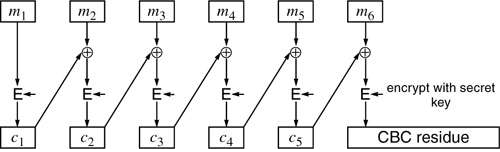
\includegraphics[height=4cm, width=12cm, keepaspectratio]{Immagini/Capitolo3/residuo_CBC.png}}
	\caption{Residuo CBC \label{fig:residuo_CBC}} 	
\end{figure}
Il calcolo del residuo CBC richiede la conoscenza della chiave segreta $K$, quindi se un avversario modifica $m$ in $m’$ allora $res_{CBC}(m’)$ sarà diverso da $res_{CBC}(m)$ (c'è solo 1 possibilità su $2^64$ che siano uguali) perchè l'avversario non è in grado di calcolare $res_{CBC}(m’)$ senza conoscere la chiave segreta $K$. \\
Il destinatario del messaggio calcola il residuo del messaggio in chiaro ricevuto, e verifica che sia uguale al residuo ricevuto; se i residui coincidono deduce che (con elevata probabilità) il residuo ricevuto è stato calcolato da qualcuno che conosce la chiave segreta, i.e. il mittente è autentico.\\
\\
In molte applicazioni non è necessario proteggere la confidenzialità, ma solo l'autenticità; in questi casi si può trasmettere il testo in chiaro più il residuo. Tuttavia, è assai frequente la necessità di
proteggere contemporaneamente confidenzialità e autenticità: se il messaggio $m$ è un singolo blocco, ciò può ottenersi con una semplice cifratura a chiave segreta. Nel caso di un messaggio multi blocco qual è la
trasformazione equivalente?
\subsection{Assicurare confidenzialità e autenticità}
Dato un messaggio $m$:
\begin{itemize}
\item per assicurare la \textbf{confidenzialità} di $m$ basta cifrarlo in modalità CBC
\item per assicurare l'\textbf{autenticità} di $m$ basta inviare $res_{CBC}(m)$ più $m$ in chiaro
\end{itemize}
Allora a prima vista la soluzione riportata in \figurename ~\ref{fig:residuo_CBC_1} sembrerebbe assicurare confidenzialità e autenticità:
\begin{figure}[htbp]
	\centering%
	\subfigure%
	{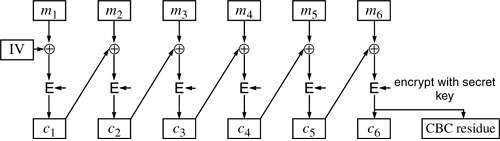
\includegraphics[height=4cm, width=12cm, keepaspectratio]{Immagini/Capitolo3/residuo_CBC_1.png}}
	\caption{Assicurare confidenzialità e autenticità: soluzione 1 \label{fig:residuo_CBC_1}} 	
\end{figure}
In realtà tale soluzione è chiaramente errata, infatti consiste nell'inviare il messaggio cifrato nella modalità CBC ($E_{CBC}(K, IV, m)$) ripetendo soltanto l'ultimo blocco cifrato ($res_{CBC}(m)$); così chiunque voglia alterare il messaggio deve solo modificare uno o più blocchi cifrati con CBC e inviare il nuovo messaggio ripetendo due volte l'ultimo blocco cifrato. \\
Quindi inviare il residuo CBC in aggiunta al messaggio cifrato con CBC non aumenta la sicurezza. \\ 
Si noti infatti che per autenticità (integrità) intendiamo che un calcolatore è in grado di rilevare automaticamente se il messaggio è stato alterato. Usando CBC da solo, allora, non è possibile rilevare in
modo automatico eventuali modifiche di un messaggio, poiché ogni stringa di bit, comunque venga generata, viene decifrata in "qualcosa", e gli ultimi 64 bit di quella stringa sono il suo residuo CBC corretto; in questo modo chiunque intercetti il testo cifrato può modificarlo, e un computer a destinazione decifrerà il risultato, che potrebbe essere assolutamente privo di senso, senza essere consapevole che quanto ottenuto è di fatto spazzatura. \\
Un utente umano si renderebbe conto che il testo cifrato è stato alterato, a meno che la modifica non sia stata eseguita da un avversario in modo "pulito", ma un computer non è in grado di farlo se non si
aggiunge un controllo di integrità.\\ \\
Un'alternativa potrebbe essere calcolare il residuo CBC del messaggio $res_{CBC}(m)$, allegarlo al testo in chiaro $m$, e cifrare con CBC la concatenazione $m|res_{CBC}(m)$ (\figurename ~\ref{fig:residuo_CBC_2})
\begin{figure}[htbp]
	\centering%
	\subfigure%
	{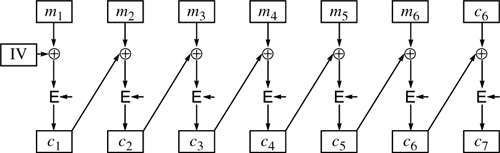
\includegraphics[height=4cm, width=12cm, keepaspectratio]{Immagini/Capitolo3/residuo_CBC_2.png}}
	\caption{Assicurare confidenzialità e autenticità: soluzione 2 \label{fig:residuo_CBC_2}} 	
\end{figure}
In realtà neanche questa soluzione funziona, infatti: $c_{7} = res_{CBC}(m) = E(K, c_{6} \oplus c_{6}) = E(K, 000 … 0)$, cioè il residuo CBC è una stringa ottenuta cifrando con la chiave segreta una stringa di 64 bit a 0, quindi il residuo CBC non dipende da $m$ e non può offrire alcune protezione di integrità.\\ \\
Come altra alternativa, supponiamo di calcolare un checksum non crittografico $CRC(m)$ (ad esempio, un CRC) del messaggio $m$ e di appenderlo alla fine di $m$, e di cifrare con CBC il tutto: $m| CRC(m)$, secondo lo schema in \figurename ~\ref{fig:residuo_CBC_3}
\begin{figure}[htbp]
	\centering%
	\subfigure%
	{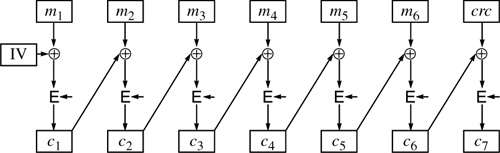
\includegraphics[height=4cm, width=12cm, keepaspectratio]{Immagini/Capitolo3/residuo_CBC_3.png}}
	\caption{Assicurare confidenzialità e autenticità: soluzione 3 \label{fig:residuo_CBC_3}} 	
\end{figure}
Questa soluzione "quasi" funziona: è vulnerabile ad attacchi molto sottili se il CRC è corto, d'altro canto checksum non crittografici più lunghi sono "sospetti". \\ 
\subsubsection{Soluzione sicura}
Viene considerata una soluzione sicura quella che riesce a proteggere la confidenzialità di un messaggio $m$ cifrandolo con CBC, e l'integrità di $m$ con un residuo CBC, a patto che vengano usate due chiavi distinte, $K$ e $K'$:
\begin{itemize}
\item confidenzialità: $E_{CBC}(K, IV, m)$
\item integrità: $res_{CBC}(K', IV, m)$
\end{itemize}
Chiaramente ciò comporta una notevole perdita di efficienza, infatti il costo computazionale è duplicato rispetto al
costo della sola cifratura CBC. \\
Sono state proposte tecniche più rapide, ma generalmente presentano sempre dei "sottili difetti" crittografici (se tali difetti siano seri o meno dipende dal tipo di applicazione e dall'intelligenza dell'avversario); alcune di queste tecniche sono:
\begin{itemize}
\item \textbf{CBC con un Checksum Crittografico Debole}: Visto che l'uso di checksum non crittografici in CBC risulta poco sicuro, e che checksum crittografici di qualità sono computazionalmente dispendiosi, è stato proposto di usare checksum crittografici "deboli". Complessivamente dovrebbe essere una soluzione sicura, infatti lo sforzo computazionale per violare il checksum debole va moltiplicato per le limitazioni derivanti dal fatto che è usato
in una cifratura CBC. Sebbene non ci sono ragioni per sostenere che tale schema sia insicuro, CBC con checksum crittografici deboli non ha riscosso successo (si consideri che Kerberos IV usa un checksum crittografico debole per la protezione d'integrità fuori da uno schema di cifratura e sembra che non sia mai stato violato!)
\item \textbf{Cifratura CBC e Residuo CBC con Chiavi Correlate}: anziché usare due chiavi completamente indipendenti per la cifratura CBC e per il calcolo del residuo, un trucco usato in Kerberos V è impiegare una versione modificata della chiave in una delle due operazioni. Cambiare un singolo bit dovrebbe essere sufficiente, ma Kerberos invece somma ($\oplus$ XOR) la chiave con la costante a 64 bit $F0F0F0F0F0F0F0F0_{16}$; tale soluzione preserva la parità della chiave e non trasforma mai una chiave non-debole in una chiave debole. Il fatto di avere una chiave matematicamente correlata all'altra (in alternativa alla scelta di due numeri random come chiavi) non introduce particolari debolezze, ma non introduce neanche particolari vantaggi (in generale, distribuire una coppia di chiavi non è più difficile di distribuirne solo una, e il fatto che due chiavi siano matematicamente correlate non riduce il carico computazionale, l'unico vantaggio nel derivare una chiave dall'altra lo si ha quando si dispone di un sistema/servizio per la distribuzioni di chiavi singole che non è estendibile al caso di coppie di chiavi).
\item \textbf{CBC con Hash Crittografico}: un altro approccio è concatenare un messaggio m con il suo un hash
crittografico $h(m)$, tipicamente 128 bit, e cifrare con CBC il tutto, $m|h(m)$. Tale soluzione è probabilmente sicura, sebbene non sia stata adeguatamente studiata, visto che gli schemi moderni usano hash cifrati con chiavi richiede due fasi crittografiche (come nel caso della cifratura CBC più il residuo CBC con chiavi distinte), ma è più efficiente se la funzione di hash è più veloce dell'algoritmo di cifratura 
\item \textbf{Offset Codebook Mode (OCB)}: OCB è uno dei molti modi che permette di ottenere cifratura e protezione di integrità effettuando soltanto una singola fase di cifratura. OCB e altre tecniche simili sono molto recenti per
avere un supporto di studi e test, spesso sono gravate da licenze/patenti, ma sembra molto probabile che una o più di
queste tecniche diventi alla fine il modo standard per ottenere protezione di integrità e di confidenzialità.
\end{itemize}

\section{Cifratura multipla DES}
\subsection{Cifratura multipla EDE o 3DES}
In generale, ogni schema di cifratura può essere reso più sicuro ricorrendo alla cifratura multipla.
Nel caso di DES, è universalmente ritenuta sicura la procedura nota come EDE.
\textbf{E}ncrypt-\textbf{D}ecrypt-\textbf{E}ncrypt (o 3DES, \textbf{triplo DES}):
\begin{itemize}
\item $c = E(K_{1},D(K_{2},E(K_{1},m))) = (E_{1} o D_{2} o E_{1})(m)$
\item $m = D(K_{1},E(K_{2},D(K_{1},c))) = (D_{1} o E_{2} o D_{1})(c)$
\end{itemize}
La cifratura multipla EDE è di fatto un meccanismo per incrementare la lunghezza della chiave DES. Sebbene sia stata introdotta per arrivare ad uno standard sicuro basato su DES, in linea di principio è applicabile anche ad altri schemi
di cifratura, ed esempio ad IDEA, ma è più importante nel caso di DES poiché la chiave DES è notoriamente considerata troppo corta.\\ \\
Si è visto che uno schema di crittografia presenta sempre due funzioni, note come cifratura e decifratura; tali funzioni sono l'una l'inversa dell'altra, i.e.: ciascuna prende in input un blocco di dati $m$, e restituisce il corrispondente blocco offuscato $c$ tale che, applicando a $c$ l'altra funzione si ottiene $m$. Ha quindi senso applicare la "funzione di decifratura" $D(K, m)$ al testo in chiaro $m$ per cifrarlo e poi applicare la "funzione di cifratura" $E(K, D(K, m))$ per decifrare quanto ottenuto riottenendo il testo in chiaro $m$; ma in definitiva ha poco senso chiamare $E(K, m)$ "funzione di cifratura", e $D(K, m)$ "funzione di decifratura", poiché i ruoli di tali funzioni sono interscambiabili. Conviene chiamarle semplicemente \textbf{funzione $E()$} e \textbf{funzione $D()$} (tuttavia, spesso si continuerà a chiamarle funzione di cifratura e funzione di decifratura).\\ \\
Realizzare una cifratura multipla non è banale, specie se si desidera anche ottenere un cifrario a flusso a partire da un cifrario a blocchi. \\
Il metodo standard per usare EDE è il seguente: vengono usate due chiavi (e non tre), $K_{1}$ e $K_{2}$ e ogni blocco di testo in chiaro $m_{i}$ è sottoposto prima ad $E_{1}()$ (cioè viene eseguito $E(K_{1}, m)$), poi a $D_{2}()$ (cioè viene eseguito $D(K_{2}, E(K_{1}, m))$) e in fine ancora ad $E_{1}()$ (cioè viene eseguito $E(K_{1}, D(K_{2},
E(K_{1}, m)))$).\\
Quanto ottenuto è di fatto un nuovo schema di cifratura a chiave segreta (\figurename ~\ref{fig:EDE}): un blocco di 64 bit in input è mappato in un altro blocco di 64 bit in output; il processo è invertibile se si conoscono le chiavi, altrimenti è di fatto impraticabile risalire dall'output all'input.
\begin{figure}[htbp]
	\centering%
	\subfigure%
	{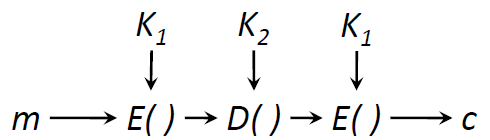
\includegraphics[height=2cm, width=10cm, keepaspectratio]{Immagini/Capitolo3/EDE.png}}
	\caption{Cifratura EDE o 3DES \label{fig:EDE}} 	
\end{figure}
La decifratura EDE è semplicemente il processo inverso (\figurename ~\ref{fig:DED}):
\begin{figure}[htbp]
	\centering%
	\subfigure%
	{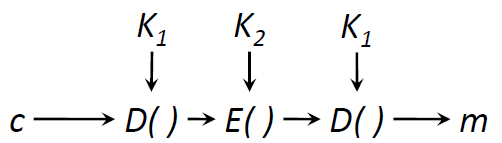
\includegraphics[height=2cm, width=10cm, keepaspectratio]{Immagini/Capitolo3/DED.png}}
	\caption{Decifratura EDE \label{fig:DED}} 	
\end{figure}
\subsection{EDE con CBC Outside/Inside}
Per ottenere un cifrario a flusso (i.e. la corrispondente modalità operativa di flusso) a partire dal cifrario a blocchi EDE, viene usata la modalità operativa \textbf{CBC outside}, i.e. le tre funzioni $E_{1}()-D_{2}()-E_{1}()$ vengono applicate a ciascun blocco, ma il concatenamento CBC viene eseguito soltanto una volta (\figurename ~\ref{fig:EDE_CBC_Out}).\\ 
\begin{figure}[htbp]
	\centering%
	\subfigure%
	{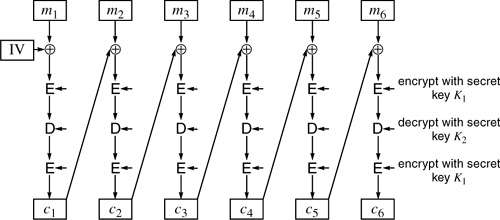
\includegraphics[height=4cm, width=12cm, keepaspectratio]{Immagini/Capitolo3/EDE_CBC_Out.png}}
	\caption{EDE con CBC Outside \label{fig:EDE_CBC_Out}} 	
\end{figure}
Il cifrario a flusso è ottenibile anche con un concatenamento \textbf{CBC inside}, i.e. si considerano una cascata di tre concatenamenti CBC (semplificando alcuni passaggi): prima utilizzando $CBC-E_{1}()$, poi utilizzando $CBC-D_{2}()$ e infine utilizzando ancora $CBC-E_{1}()$ (\figurename ~\ref{fig:EDE_CBC_In}).
\begin{figure}[htbp]
	\centering%
	\subfigure%
	{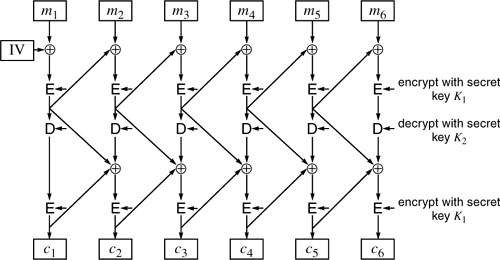
\includegraphics[height=4cm, width=12cm, keepaspectratio]{Immagini/Capitolo3/EDE_CBC_In.png}}
	\caption{EDE con CBC Inside \label{fig:EDE_CBC_In}} 	
\end{figure}
\subsubsection{CBC Outside vs Inside}
Il 3DES comunemente usato nelle applicazioni esegue un concatenamento CBC esterno: ad ogni blocco viene applicata la cifratura tripla e il concatenamento CBC viene fatto una sola volta sui blocchi cifrati. L'alternativa sarebbe cifrare completamente il messaggio con $K_{1}$ e CBC, poi decifrare il risultato con $K_{2}$ e CBC, e in fine cifrare di nuovo quanto ottenuto con $K_{1}$ (CBC interno).\\
Quali sono le implicazioni di queste scelte?\\ \\
Si è visto che con CBC è possibile fare una modifica predittiva sul testo in chiaro $m_{n}$ (ad esempio invertire il bit $x$) invertendo il bit $x$ nel blocco cifrato $c_{n-1}$; ciò comporta però l'effetto collaterale di modificare
in modo imprevedibile il blocco $m_{n-1}$, la possibilità di sfruttare questa debolezza dipende dal tipo di applicazione.\\ \\
Con CBC esterno, un avversario può ancora sferrare questo tipo di attacco (il fatto che la cifratura è fatta con un triplo DES è del tutto ininfluente): un avversario che inverte il bit $x$ di un blocco cifrato $c_{n-1}$ modificherà completamente e in modo imprevedibile il blocco di testo in chiaro $m_{n-1}$ (il blocco di testo in chiaro $m_{n}$ avrà il bit $x$ invertito e tutti i blocchi di testo in chiaro diversi da $m_{n-1}$ e $m_{n}$ saranno invariati.\\ \\
Con CBC interno, una modifica ad un blocco cifrato $c_{n}$ altera in modo imprevedibile tutti i blocchi di testo in
chiaro dal blocco $m_{n}$ fino alla fine del messaggio. Per questo CBC interno è più sicuro di CBC esterno, e forse
dovrebbe essere la scelta migliore; tuttavia, in alcuni casi è preferibile che la modifica di un blocco cifrato non si propaghi completamente nel resto del messaggio, i.e. sarebbe preferibile che lo schema di cifratura sia autosincronizzante (dopo un piccolo numero di blocchi corrotti, il testo in chiaro inizierà ad essere nuovamente decifrato correttamente). \\
Un altro vantaggio di CBC interno riguarda l'efficienza: triplicando l'uso di hardware e pipeline per le cifrature si può ottenere complessivamente una velocità pari a quella di una singola cifratura (con CBC esterno ciò non è possibile).\\
CBC interno presenta comunque delle sottili vulnerabilità se un avversario può esaminare l'output e fornire del testo in chiaro scelto e $IV$.\\ \\
Una ragione per la quale CBC esterno è più usato nonostante i suoi svantaggi è che la cifratura EDE può considerarsi a tutti gli effetti un nuovo schema di cifratura (a chiave segreta) a blocchi che usa una chiave di 112 bit, perciò può essere utilizzata con ciascun metodo di concatenamento (OFB, ECB, CFB, CTR e CBC).
\subsection{Cifrature multiple}
Ovviamente, più volte un blocco è cifrato più elevata è la sua sicurezza, ma ogni cifratura è computazionalmente costosa, perciò è fondamentale che una schema di cifratura sia efficiente oltre che efficace: l'obiettivo è garantire un livello di sicurezza elevato con il minimo sforzo computazionale. \\
Proviamo allora a valutare il rapporto sicurezza / costo computazionale nei seguenti casi:
\begin{itemize}
\item cifratura \textbf{doppia} con la \textbf{stessa chiave}
\item cifratura \textbf{doppia} con \textbf{due chiavi diverse}
\item cifratura \textbf{tripla} con \textbf{due chiavi diverse}
\item cifratura \textbf{tripla} con \textbf{tre chiavi diverse}
\end{itemize}
\subsubsection{Cifratura doppia con una stessa chiave}
Supponiamo di non volere il disagio di leggere in due chiavi, secondo lo schema in \figurename ~\ref{fig:Cif_doppia_stessaK} (o in alternativa secondo uno degli schemi in \figurename ~\ref{fig:Cif_doppia_stessaK_alternative}), ma cifrare due volte consecutive con la stessa chiave aumenta la sicurezza?
\begin{figure}[htbp]
	\centering%
	\subfigure%
	{
\includegraphics[height=2cm, width=10cm, keepaspectratio]{Immagini/Capitolo3/Cif_doppia_stessaK.png}}
	\caption{Schema di cifratura doppia con una stessa chiave \label{fig:Cif_doppia_stessaK}} 
	\subfigure%
	{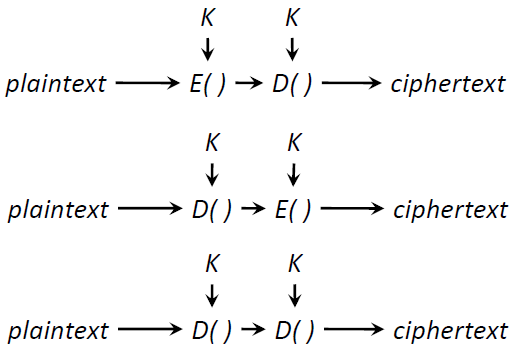
\includegraphics[height=6cm, width=10cm, keepaspectratio]{Immagini/Capitolo3/Cif_doppia_stessaK_alternative.png}}
	\caption{Schemi alternativi di cifratura doppia con una stessa chiave \label{fig:Cif_doppia_stessaK_alternative}} 
\end{figure}
Cifrare due volte con la stessa chiave $K$ risulta non essere molto più sicuro di eseguire una singola cifratura con $K$, poiché una ricerca esaustiva nello spazio della chiave richiede ancora, nel caso peggiore, $2^{56}$ tentativi, dove ogni tentativo ha un costo computazionale duplicato; perciò l'avversario deve eseguire una decifratura doppia, ma raddoppiare lo sforzo computazionale non è considerato in generale un aumento significativo della sicurezza, soprattutto tenendo conto che anche l'efficienza risulta essere dimezzata.
\subsubsection{Cifratura doppia con due chiavi}
Se cifrare due volte consecutive, con due chiavi diverse $K_{1}$ e $K_{2}$, avesse l'effetto di raddoppiare la chiave (da 56
a 112 bit), allora la cifratura doppia sarebbe sufficiente... (scopriremo che non è così)\\
Supponiamo di eseguire una cifratura doppia, con due chiavi $K_{1}$ e $K_{2}$ (secondo lo schema in \figurename ~\ref{fig:Cif_doppia_dueK}), su un singolo blocco da 64 bit (trascuriamo ogni schema di concatenamento e concentriamoci sui cifrari a blocchi); 
\begin{figure}[htbp]
	\centering%
	\subfigure%
	{
\includegraphics[height=2cm, width=10cm, keepaspectratio]{Immagini/Capitolo3/Cif_doppia_dueK.png}}
	\caption{Schema di cifratura doppia con due chiavi diverse \label{fig:Cif_doppia_dueK}} 
\end{figure}
in apparenza, sembra che l'uso di due chiavi diverse equivalga a raddoppiare la lunghezza della chiave (infatti un attacco brute force deve indovinare sia $K_{1}$ che $K_{2}$ per ottenere il testo in chiaro da quello cifrato), tuttavia esiste un attacco più sofisticato che richiede approssimativamente soltanto un raddoppio del costo computazionale necessario a violare DES (singolo). Si tratta di un attacco difficilmente praticabile, ma il fatto che esista spinge a ricercare schemi di cifratura più sicuri: di fatto la cifratura DES con due chiavi non è considerata.
sicura. (Vedremo più avanti l'attacco a DES doppio)
\subsection{Cifratura tripla con solo due chiavi}
3DES effettua una cifratura tripla, ma usa solo due chiavi. \\
Ovviamente con tre chiavi distinte si ha una maggiore, tuttavia, è ormai opinione comune che usare $K_{1}$ due
volte è sufficientemente sicuro, perciò non è necessario generare, trasmettere e memorizzare una terza chiave. Inoltre 112 bit di chiave mettono al riparo da attacchi di tipo brute force e nessun attacco diverso da quello a forza bruta è noto per EDE. Si noti che alcuni sistemi implementano 3DES con tre chiavi indipendenti, ma questo non è lo standard.\\ \\
Una ragione "esoterica" per l'uso di due sole chiavi è la seguente: in molte applicazioni (es. UNIX Password Hash) una proprietà importante di un sistema crittografico è che, data una coppia <plaintext, ciphertext>, deve essere impraticabile trovare qualche chiave che mappa il testo in chiaro in quello cifrato (con blocchi di 64 bit e chiavi di 112 bit ci saranno molte di queste chiavi); usando EDE con tre chiavi diverse, è semplice trovare una tripla di chiavi che mappa un dato testo in chiaro in un dato testo cifrato però, nel caso in cui $K_{1} = K_{3}$ il problema diventa impraticabile.\\
Si noti infine che la chiave $K_{2}$ è usata in modalità di decifratura, cioè nella funzione di decifratura
$D()$ di EDE. Tale scelta non serve ad aumentare il livello di sicurezza (si poteva usare $K_{2}$ in modalità di
cifratura ottenendo uno schema di tipo EEE); una possibile ragione è che se $K_{1} = K_{2}$ allora EDE
equivale ad un semplice DES, quindi è possibile interoperare con un sistema DES semplice.
\section{Attacco a DES doppio}
Si assuma che un avversario disponga di qualche coppia $<plaintext, ciphertext>$: $<m_{1},c_{1}> , <m_{2},c_{2}> , <m_{3},c_{3}> , ...$ dove $c_{i} = E(K_{2}, E(K_{1}, m_{i}))$ è ottenuto eseguendo una cifratura doppia di $m_{i}$ con $K_{1}$ e $K_{2}$ e desideri trovare le chiavi $K_{1}$ e $K_{2}$. \\
Per farlo deve:
\begin{itemize}
\item Costruire una tabella $A$ con $2^56$ entry, di cui ogni entry è una coppia $<K_{i}, r = E(K_{i}, m_{1})>$ e ordinarla in base al valore numerico di $r$;
\item Costruire una tabella $B$ con $2^56$ entry, di cui ogni entry è una coppia $<K_{i}, r = D(K_{i}, c_{1})>$ e ordinarla in base al valore numerico di $r$;
\item Ricercare nelle due tabelle (ordinate) le entry corrispondenti, cioè con lo stesso valore di $r$, e.g. $<K_{A},r>$ dalla tabella $A$ e $<K_{B},r>$ dalla tabella $B$ ($K_{A}$ è la candidata per $K_{1}$ e $K_{B}$ è la candidata per $K_{2}$); questo è necessario perché, essendo $r = E(K_{A}, m_{1})$ e $r = D(K_{i}, c_{1})$, allora $c_{1} = E(K_{B}, E(K_{A}, m_{1}))$;
\item Visto che, in generale, si otterrà più di una coppia candidata per $<m_{1},c_{1}>$, per ciascuna si esegue il test rispetto a $<m_{2},c_{2}>$ e, finchè ci sono più coppie candidate, si eseguono i test con le successive coppie $<m_{i},c_{i}>$: la coppia corretta è quella che passa tutti i test, mentre quelle errate ne dovranno fallire qualcuno (dimostreremo che sono sufficienti tre tentativi per trovare una coppia corretta). 
\end{itemize} 
L'attacco a DES doppio appena descritto è difficilmente praticabile (dover costruire una tabella di $2^56$ entry è sicuramente scoraggiante); tuttavia, l'esistenza di un attacco è una ragione sufficiente per decidere di usare DES triplo (DES doppio potrebbe essere sufficiente, ma DES triplo è più sicuro e non e molto più complesso da realizzare).
\subsection{Stima dei tentativi}
Vediamo quante coppie candidate ci saranno mediamente dopo la prima ricerca nelle due tabelle.\\
Sia $cc_{1}$ il numero atteso di coppie candidate ottenute dopo la prima ricerca.
Visto che i possibili blocchi di 64 bit sono $2^64$ e che le entry in ciascuna tabella sono $2^56$ la probabilità $P_{bt}$ che un blocco sia in una tabella è $P_{bt} = 2^56 / 2^64 = 2^-8$, mentre la probabilità $P_{c1}$ che un blocco sia in entrambe le tabelle (e che quindi identifichi una coppia candidata) è $P_{c1} = 2^-8 \times 2^-8 = 2^-16$. \\
Ora, $cc1 \approx Pc1 ∙ numero blocchi = 2^64 / 2^16 = 2^48$, vale a dire che ci sono $2^48$ coppie candidate errate.\\
Consideriamo adesso la probabilità $P_{c2}$ che una coppia candidata soddisfi anche il secondo test: questa vale $P_{c2} \approx 2^-64$. \\
La probabilità $P_{e2}$ di trovare un coppia candidata errata dopo il secondo test vale $P_{e2} = 2^48 / 2^64$ e al terzo test si avrà $P_{e2} = 2^48 / 2^128 = 2^-80$: quindi la probabilità di trovare un falso positivo dopo tre test
è di fatto nulla e dopo tre test si ottiene un'unica coppia candidata che è quella corretta. 
\chapter{Funzioni Crittografiche di Hash}
\section{Introduzione}
Una funzione di hash (o semplicemente hash o message digest) è una funzione unidirezionale (o one-way), del tipo h: $\{0, 1\}^{*} \rightarrow \{0, 1\}^{b}$, dove:

\begin{itemize}
	\item $\{0, 1\}^{*}$: spazio delle stringhe binarie di lunghezza qualsiasi
	\item $\{0, 1\}^{b}$: spazio delle stringhe binarie di lunghezza b bit
\end{itemize}

La funzione di hash è considerata unidirezionale (one-way) perché in genere è impraticabile capire quale input corrisponda ad un dato output. Sia \textbf{h()} una funzione di hash, allora \textbf{h()} è una \textbf{funzione di hash sicura} se rispetta le seguenti proprietà:

\begin{itemize}
	\item \textbf{resistenza alla preimmagine}: fissato un hash $\hbar$ è computazionalmente impraticabile trovare un messaggio m tale che $h(m) = \hbar$
	\item \textbf{resistenza alle collisioni}: è computazionalmente	impraticabile trovare due messaggi m1 e m2 aventi lo 	stesso digest h(m1) = h(m2), le proprietà precedenti implicano la seguente
	\item \textbf{resistenza alla seconda preimmagine}: dato un messaggio m, è computazionalmente impraticabile trovare un	messaggio m’ avente lo stesso digest $h(m) = h(m’)$
\end{itemize}


Si useranno i termini hash e message digest in modo intercambiabile; la funzione di hash del NIST è chiamata \textbf{SHA-1}: Secure Hash Algorithm mentre l'acronimo MD degli algoritmi \textbf{MD2}, \textbf{MD4} e \textbf{MD5} sta per Message Digest. Tutti gli algoritmi di digest/hash di base fanno la stessa cosa: prendono in input un messaggio di lunghezza variabile, e restituiscono in output una quantità avente lunghezza prefissata. \newline \newline

\subsubsection{Randomicità della funzione}
Dato un messaggio \textbf{m}, il digest \textbf{h(m)} viene calcolato in modo \textbf{deterministico}. Tuttavia, l'output della funzione di hash dovrebbe apparire il più possibile casuale. Dovrebbe essere impossibile, senza applicare la funzione di hash, predire una qualsiasi porzione dell'output: per ogni sottoinsieme (di posizioni) di bit nel digest \textbf{h(m)} dovrebbe essere possibile ottenere due messaggi m1 e m2 tali che h(m1) e h(m2) presentino gli stessi bit in quelle posizioni \textbf{soltanto procedendo in modo esaustivo}. \newline \newline

Chiaramente, ci sono molti messaggi distinti che sono mappati in uno stesso digest h(m); m ha lunghezza arbitraria, mentre il digest h(m) ha una lunghezza prefissata, ad esempio 128 bit. Se m ha una lunghezza di 1000 bit e h(m) di 128 bit ci sono in media 2872 messaggi che sono mappati in uno stesso digest e dopo molti tentativi, due messaggi aventi lo stesso digest si trovano sicuramente. Tuttavia, per "molti tentativi" si intende un numero talmente grande che è di fatto impossibile. Considerando una buona funzione di digest a 128 bit, è necessario provare approssimativamente $2^{128}$ possibili messaggi prima di ottenere un messaggio avente un particolare digest, o $2^{64}$ messaggi prima di trovarne due aventi lo stesso digest (trovare cioè due messaggi che collidono).

\section{Esempio di Applicazioni}
Un’applicazione delle funzioni di hash crittografiche è il calcolo dell’impronta digitale di un programma o di un documento di cui si desiderano monitorare eventuali modifiche : se il message digest h(p) del programma p è noto e se h(p) è memorizzato in modo sicuro (cioè non può essere modificato da utenti non autorizzati) allora nessun utente non autorizzato può modificare p senza essere scoperto perché non sarà in grado di trovare un diverso programma p’ tale che h(p’) = h(p).
Quindi sia h:$\{0, 1\}^{*} \rightarrow \{0, 1\}^{b}$ una funzione di hash siano $m_{1}, m_{2}, ..., m_{N}$ N messaggi arbitrariamente
scelti in ${0, 1}^{*}$. \\
\textbf{DOMANDA}: quanto deve valere N per avere una probabilità di 0.5 che due messaggi $m_{i}, m_{j}$ abbiano lo stesso hash?

Una prima stima di N (affinché ci sia 0.5 di possibilità di collisione), per difetto, è la seguente :
\begin{itemize}
\item $k = 2^{b}$: numero totale di possibili hash
\item $\frac{1}{k}$ : probabilità che una coppia di messaggi collida
\item $\textbf{Ipotesi}$: gli eventi considerati sono mutuamente esclusivi 
	\begin{itemize}
		\item $\Pr\{h(mi) = h(mj) \mbox{ OR } h(mp) = h(mq)\} = \Pr\{h(mi) = h(mj)\} + \Pr\{ h(mp) = h(mq)\}$
	\end{itemize}
\end{itemize}
 
A rigore tale ipotesi non è soddisfatta, molti eventi hanno intersezione non nulla, perciò la stima ottenuta della probabilità è per eccesso e ciò si traduce in una stima per difetto di N $(\Pr\{E1 \mbox{ OR } E2\} = \Pr\{E1\} + \Pr\{E2\} - \Pr\{E1 \bigcap E2\})$.
Si ha una probabilità di 0.5 se si considerano $k/2$ coppie, perciò $N(N - 1)/2 = k/2$ e ipotizzando $N >> 1$ si ha $N = k^{1/2} = 2^{b/2}$.

Una seconda stima, più accurata di N è la seguente:
\begin{itemize}
\item P: probabilità che almeno una coppia di messaggi collida
\item $P^{*}$: probabilità che tutte le coppie di messaggi abbiano digest diversi, quindi $P = 1 - P^{*}$
\item \textbf{Ipotesi}: gli eventi considerati sono indipendenti
	\begin{itemize}
		\item $\Pr\{h(mi) \neq h(mj) \mbox{ AND } h(mp) \neq h(mq)\} = \Pr\{h(mi) \neq h(mj)\} * \Pr\{ h(mp) \neq h(mq)\}$
	\end{itemize}
\end{itemize}

A rigore tale ipotesi non è soddisfatta, gli eventi non sono del tutto indipendenti quindi la stima ottenuta della probabilità P è per difetto e ciò si traduce in una stima per eccesso di N ($\Pr\{E1 \mbox{ AND } E2\} = \Pr\{E1\} * \Pr\{E1|E2\}$).
Nella ipotesi di eventi indipendenti si ha $P = 1 - P^{*} = 1 - (1 - 1/k)^{\frac{N(N - 1)}{2}}$, e ipotizzando che k >> 1 si ottiene che $P \approx 1 - e^{- N(N - 1)/2k}$, ponendo pertanto $P\geq1/2 si ottiene che e^{- N(N - 1)/2k} \leqslant 1/2 = e^{-ln2}$; da cui si ottiene che $N(N - 1)/2 \geq (ln2)k$ e, ipotizzando che N >> 1, $N \geqslant (2ln2)^{1/2} \cdot k^{1/2} = (2ln2)^{1/2} \cdot 2^{b/2}$.

Una terza stima ancor più corretta si può ottenere utilizzando la modalità di calcolo utilizzata anche nel paradosso del compleanno :
\begin{itemize}
\item P: probabilità che almeno una coppia di messaggi collida
\item $P^{*}$: probabilità che tutte le coppie di messaggi abbiano digest diversi, quindi $P = 1 - P^{*}$
\item $k = 2^{b}$: numero di possibili hash
\end{itemize}
Si consideri inoltre la seguente notazione:
\begin{itemize}
\item $P_{2^{*}}$: la probabilità che h(m2) sia diverso da h(m1)
\item $P_{3^{*}}$: la probabilità che h(m3) sia diverso da h(m2) e h(m1)
\item ...
\item $P_{i^{*}}$: la probabilità che h(mi) sia diverso da h(mj), $\forall 1\leq j \leq i-1$
\item ...
\item $P_{N^{*}}$: la probabilità che h(mN) sia diverso da h(mj), $\forall 1\leq j \leq N-1$
\end{itemize}
Da tutto ciò segue che $P^{*}=P_{2^{*}}*P_{3^{*}}*...*P_{i^{*}}*...*P_{N^{*}}=
(k - 1)/k*(k - 2)/k*...*(k - N + 1)/k = \frac{k!}{(k^{N}*(k - N)!)}\Rightarrow P^{*} = \frac{k!}{(k^{N}*(k - N)!)}$.
Questa è la stima esatta di $P^{*}$, si nota che il precedente valore di $P^{*}$ si può approssimare con $1 - e^{- N(N - 1)/2k}$.

\section{Lunghezza di un messaggio di Digest}
Quanti bit deve avere l’output di una funzione di hash in modo tale che nessuno sia in grado di trovare due messaggi aventi lo stesso digest?
Se il digest ha b bit, per trovare due messaggi aventi lo stesso digest, è necessario considerare circa $2^{b/2}$ messaggi, se il digest è lungo 64 bit, la ricerca esaustiva in uno spazio di circa $2^{32}$ elementi può essere fattibile mentre se il digest è lungo 128 bit si ritiene che una ricerca in uno spazio di $2^{64}$ elementi sia impraticabile dato l’attuale stato dell’arte.
Per quale ragione è importante che una funzione crittografica di hash sia resistente alle collisioni?
Il fatto che debba essere resistente alla preeimmagine è scontato, ma la resistenza alle collisioni è veramente necessaria?? Si, dato che in alcune circostanze riuscire a trovare due messaggi con lo stesso digest può comportare dei seri problemi di sicurezza!!
Ad esempio, Alice genera una informazione $x_{A}$ e incarica Bob di calcolare un messaggio $m_{A}$ il cui contenuto deve dipendere da $x_{A}$ secondo criteri prestabiliti.
Una volta che Bob ha calcolato $m_{A}$ lo sottopone ad Alice che ne verifica l'integrità e calcola l'impronta $h(m_{A})$, la firma con la sua chiave privata e invia a Trudy il messaggio in chiaro $m_{A}$ e la sua firma.
Trudy legge il messaggio $m_{A}$ e la firma, controlla che la firma sia quella di Alice e verifica che tutto $m_{A}$ coincida con $h(m_{A})$.
\begin{figure}
	\begin{center}
	{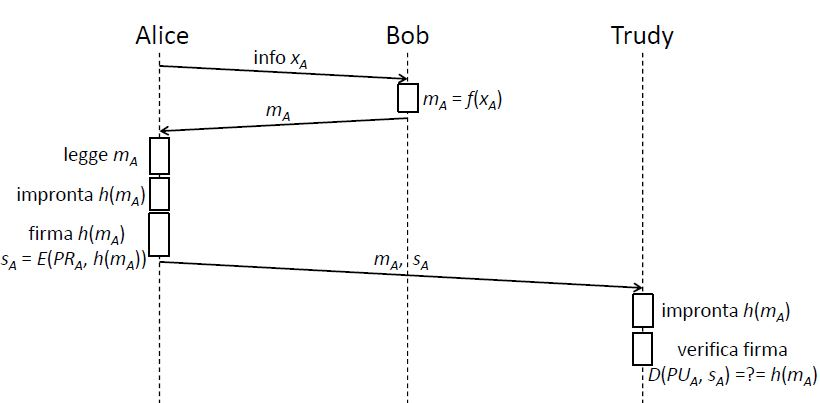
\includegraphics[height=13cm, width=13cm, keepaspectratio]{Immagini/Capitolo4/schema_hash_collisioni.JPG}}
	\end{center}
\end{figure}
Se la funzione non è resistente alla collisioni, Bob potrebbe trovare $m_{A1}$ tale che risulti $h(m_{A})= h(m_{A1})$.
Una volta che Alice ha firmato il messaggio, sostituisce $m_{A}$ con $m_{A1}$ e Trudy non si potrà mai accorgere di nulla.
\begin{figure}
	\begin{center}
	{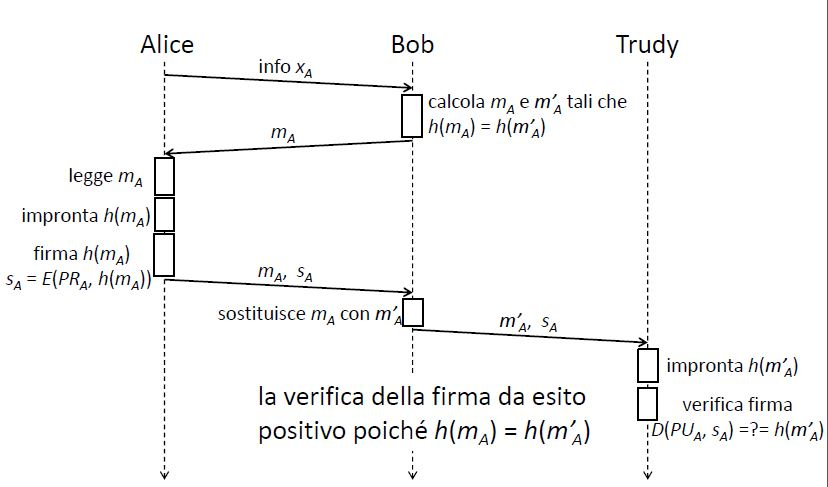
\includegraphics[height=13cm, width=13cm, keepaspectratio]{Immagini/Capitolo4/schema_hash_collisioni_1.JPG}}
	\end{center}
\end{figure}
Ma, per calcolare due messaggi con lo stesso hash, Bob può seguire il seguente approccio a forza bruta:
\begin{itemize}
\item dato $x_{A}$, calcola prima il messaggio $m_{A}$ come desiderato da Alice;
\item genera un messaggio falsato $m_{A^{'}}$;
\item esegue il test $h(m_{A})==h(m_{A}^{'})$;
\item in caso negativo ritorna al punto 2;
\end{itemize}
con questo approccio a forza bruta, però, sono necessari circa $2^{b}$ tentativi, e non $2^{b/2}$!

\section{Impieghi degli Algoritmi di Hash}
Disponendo di un segreto condiviso, l'algoritmo di hash può "sostituire" un algoritmo di crittografia a chiave segreta in ogni suo impiego. (Autenticazione a chiave segreta, Calcolo di MAC, Cifratura e Decifratura).
\subsection{Message Digest per MAC}
Un possibile schema di autenticazione a chiave segreta (composta da "sfide") è il seguente
\begin{figure}
	\begin{center}
	{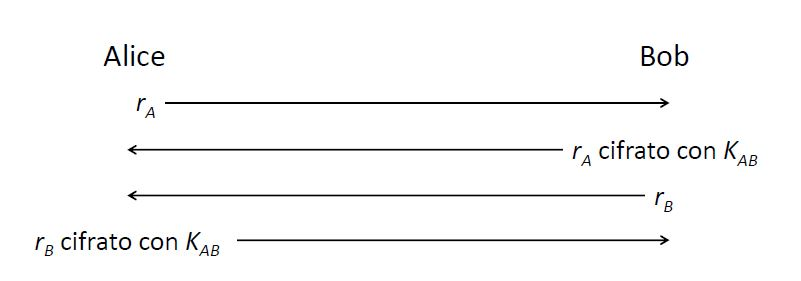
\includegraphics[height=13cm, width=13cm, keepaspectratio]{Immagini/Capitolo4/schema_autenticazione.JPG}}
	\end{center}
\end{figure}
Questo schema, purtroppo, presenta delle vulnerabilità...così come il seguente:
\begin{figure}
	\begin{center}
	{\includegraphics[height=13cm, width=13cm, keepaspectratio]{Immagini/Capitolo4/schema_autenticazione_md.JPG}}
	\end{center}
\end{figure}
Le vulnerabilità degli algoritmi di digest MD, sono note e facilmente attuabili in un possibile attacco.
Infatti, MD(m) è calcolabile da tutti coloro che conoscono m e l’algoritmo di digest MD senza conoscere la chiave 
segreta!!
Poiché, dall’input m si ottiene un messaggio mp avente lunghezza pari ad un multiplo intero di 512 bit ()mediante un opportuno padding che include, tra l’altro, la lunghezza originaria di m), mp viene decomposto in chunk (pezzi) da 512 bit il digest viene ottenuto mediante una procedura iterativa, quindi il digest all’n-esima iterazione dipende esclusivamente dall’n-esimo chunk e dal digest ottenuto all’(n – 1)-esima iterazione...il digest risultante di m è il digest ottenuto all’ultima iterazione.
Se un attaccante intercetta $\langle m, MD(K_{AB}|m) \rangle$ tra Alice e Bob, l'attaccante senza conoscere la chiave segreta $K_{AB}$ può calcolare il MAC di $\langle m^{+}, MD(K_{AB}|m^{*}) \rangle$ (dato che l'algoritmo di hash è noto) tramite l'ultimo messaggio intercettato. \\
Una possibile soluzione è che il segreto $K_{AB}$ sia messo in coda, a patto che l'algoritmo di hash sia molto resistente alle collisioni!! Un altra possibilità è quella di utilizzare come MAC un sottoinsieme arbitrario del digest MD, in questo caso, se il mio MAC è di soli 64 bit (invece di 128), l'attaccante potrebbe sempre ricostruire un messaggio da accodare...ma ha una possibilità su $2^{64}$ che il MAC ottenuto sia quello corretto.
\\
Una terza soluzione è quella di inserire il segreto $K_{AB}$ sia all'inizio che in coda del messaggio da mandare al digest MD, così che $K_{AB}$ in testa fornisca resistenza alle collisioni e $K_{AB}$ rende innocua la vulnerabilità insita negli algoritmi di hash.
Dato che ognuna delle soluzioni è equivalentemente corretta per ovviare al problema della vulnerabilità della funzione MD, per dare una piattaforma condivisa...una soluzione condivisibile da tutti, è stato introdotto il framework \textbf{HMAC} (keyed-Hash Message Authentication Code); l'algoritmo HMAC calcola due volte il digest del messaggio, e ogni volta inserisce in testa il segreto $K_{AB}$.
\subsection{Cifratura/Decifratura} 
Come faccio a cifrare con un algoritmo di hash? Devo utilizzare la funzione di hash potendo rendere tutto il processo invertibile, quindi introducendo lo XOR tra un chunk del messaggio e l' hash della chiave (genero un keypad) e ottengo un cifrario a flusso!!
\begin{figure}
	\begin{center}
	{\includegraphics[height=13cm, width=13cm, keepaspectratio]{Immagini/Capitolo4/schema_cifratura_flusso.JPG}}
	\end{center}
\end{figure}

\subsection{Algoritmi di cifratura come algoritmi di hash}
Se un algoritmo di hash/digest, può essere utilizzato come un algoritmo di cifratura...può accadere il contrario?
In genere, questo principio è utilizzato (ad esempio) per la memorizzazione degli hash delle password in UNIX.
Ma come si modifica un algoritmo di cifratura che sia resistente alle collisioni?\\
Lo schema di funzionamento (minimale) è questa
\begin{figure}
	\begin{center}
	{\includegraphics[height=13cm, width=13cm, keepaspectratio]{Immagini/Capitolo4/schema_des_come_hash.JPG}}
	\end{center}
\end{figure}
Ma questo schema funziona per soli messaggi corti e non è troppo resistente alle collisioni, sebbene $K_{PWD}$ sia ottenuta dalla pwd considerandone i primi 8 caratteri ed espansa con con i bit di parità per ogni gruppo di 8 bit.
Dato s il \textit{salt}, invero il numero di 12 bit ottenuto in modo pseudo randomico dalla pwd di ogni utente, la funzione h(pwd) si ottiene dal DES modificato che dipende dal valore di s (che determina quali bit  devono essere replicati nella fase di espansione di R da 32 a 48 bit). Infine il DES modificato è utilizzato con $K_{PWD}$ pr cifrare una costante 0 a 64 bit. Il risultato della cifratura e il salt, sono memorizzati per poter recuperare pwd.

\subsection{Hash di grandi messaggi con algoritmi di cifratura come hash}
Per l'algoritmo precedente, era stato sottolineato che era valido esclusivamente per messaggi corti.
Come si deve operare per estendere questi algoritmi a messaggi di lunghezza arbitraria?
Si può pensare di suddividere il messaggio $m = m_{1},m_{2},m_{3},...,m_{n}$, ogni $m_{i}$ viene utilizzato come input a un blocco in cascata di cifratura, alla fine della cascata ho realizzato un algoritmo di hash tramite cifratura...per un messaggio di lunghezza qualsiasi.\\
\begin{figure}
	\begin{center}
	{\includegraphics[height=10cm, width=10cm, keepaspectratio]{Immagini/Capitolo4/schema_des_come_hash_1.JPG}}
	\end{center}
\end{figure}
Purtroppo questo sistema soffre degli stessi problemi di cui soffriva il DES doppio, per ovviare ciò, basta rendere l'output di ogni blocco differente diverso dall'input del successivo, una possibile implementazione è la seguente
\begin{figure}
	\begin{center}
	{\includegraphics[height=10cm, width=10cm, keepaspectratio]{Immagini/Capitolo4/schema_des_come_hash_2.JPG}}
	\end{center}
\end{figure}

\subsection{Rainbow Tables (Opzionale)}
Le Rainbow tables sono un meccanismo per l'attacco di reverse hash. Le tables bilanciano memoria e sforzo computazionale, se fosse utilizzata solo memoria si avrebbero dei database troppo grandi per poter mappare tutte le immagini degli hash e se fosse utilizzata solo potenza computazionale servirebbe troppo tempo per poter trovare l'inverso di un hash.\\
Le Rainbow tables utilizzano delle funzioni di riduzione r(), la funzione di riduzione è una applicazione dallo spazio degli Hash allo spazio dei Plaintext, r() non è l'inversa di un algoritmo di hash; per questo, prima di avvicinarmi a una buona inversione dovrò concatenare fino a centinaia di iterazioni di $h(m) = k \longrightarrow r(k) = m^{'}$.
\begin{figure}
	\begin{center}
	{\includegraphics[height=10cm, width=10cm, keepaspectratio]{Immagini/Capitolo4/riduzione.JPG}}
	\end{center}
\end{figure}
Per popolare la table, si memorizzano solo il messaggio iniziale e il messaggio finale della catena. In questo modo, con una catena di 100 iterazioni (dato che le funzioni sono deterministiche) si risparmia uno spazio in memoria di 100 volte la grandezza della table, in confronto a memorizzare solo coppie $\langle plaintext, hash \rangle$.
Per recuperare un plaintext di un hash, si controlla se questo sia un endpoint di una qualsiasi delle catene (fase di lookup), se non lo fosse si controllano gli endpoint intermedi di ogni catena.
Appena recuperato l'hash giusto, si utilizza la catena determinata dall'inizio finchè non si trova l'hash di inizio; il messaggio che ha generato quell'hash sarà ciò che si cercava.
\begin{figure}
	\begin{center}
	{\includegraphics[height=10cm, width=10cm, keepaspectratio]{Immagini/Capitolo4/riduzione.JPG}}
	\end{center}
\end{figure}
%%\chapter{Crittografia a chiave pubblica}
<<<<<<< HEAD

La crittografia a chiave pubblica si basa su alcuni risultati nell'ambito della teoria dei numeri. Si esamineranno i seguenti schemi di cifratura a chiave pubblica: \begin{itemize}
||||||| merged common ancestors

%%Scrivere normalmente, SENZA inserire begin e end document, che sono gi� compresi nel file principale da compilare
La crittografia a chiave pubblica si basa su alcuni risultati nell'ambito della teoria dei numeri. Si esamineranno i seguenti schemi di cifratura a chiave pubblica: \begin{itemize}
=======
La crittografia a chiave pubblica si basa su alcuni risultati nell'ambito della teoria dei numeri. Si esamineranno i seguenti schemi di cifratura a chiave pubblica: 
\begin{itemize}
>>>>>>> 97170125928e81d41229ce7a4b1ea69a00151de4
\item RSA usata per cifrare e per calcolare la firma digitale
\item ElGamal e DSS, usati per la firma digitale
\item Diffie-Hellman, permette di stabilire un segreto condiviso, ma non fornisce alcun algoritmo che usa effettivamente tale segreto
\end{itemize}
<<<<<<< HEAD
L'unico aspetto comune a tutti gli algoritmi di crittografia a chiave pubblica è la presenza di due quantità correlate: una chiave segreta e una chiave pubblica.
||||||| merged common ancestors
L'unico aspetto comune a tutti gli algoritmi di crittografia a chiave pubblica � la presenza di due quantit� correlate: una chiave segreta e una chiave pubblica.
=======

L'unico aspetto comune a tutti gli algoritmi di crittografia a chiave pubblica è la presenza di due quantità correlate: una chiave segreta e una chiave pubblica.
>>>>>>> 97170125928e81d41229ce7a4b1ea69a00151de4
\section{Aritmetica modulare}
La maggior parte degli algoritmi a chiave pubblica si basano sull'aritmetica modulare: fissato un intero $ n>1 $, l'aritmetica modulare considera l'insieme degli interi non negativi minori di
$n: $\{$0, 1, 2,..., n-1$\}, effettua operazioni ordinarie come l'addizione e la moltiplicazione, e sostituisce il risultato $x$ con il resto $r$ della divisione intera di $x$ per $n$. Il risultato finale viene detto modulo n o $mod \, n$. \\
<<<<<<< HEAD
Definiamo l'inverso moltiplicativo di $k$, indicato con $k^{-1}$, come quel numero che moltiplicato per $k$ dà 1, cioè $kk^{-1} \, mod \, n = 1 \, mod \, n$. Fissato n, non tutti i numeri hanno un inverso moltiplicativo $mod \, n$. Si osservi inoltre che, se $k$ ammette un inverso moltiplicativo $mod \, n $, esiste un unico inverso moltiplicativo $k^{-1} < n$. La moltiplicazione $mod \, n$ di per sé non costituisce un cifrario sicuro,ma funziona, nel senso che la moltiplicazione per $k$ produce un mescolamento dell'input; la decifratura può ottenersi moltiplicando per $k^{-1}$.\\ Trovare un inverso moltiplicativo $k^{-1}$ nella aritmetica $mod \, n$, non è affatto banale se $n$ è molto grande. Esiste un modo efficiente per risolvere tale problema, noto come algoritmo di Euclide: \begin{itemize}
\item dati $x$ ed $n$, con $x<n$, l'algoritmo di Euclide trova il
numero $y<n$ tale che $xy \, mod \, n = 1$, ammesso che un siffatto $y$ esista.\end{itemize} 
Quali sono dunque gli inversi moltiplicativi $mod \, n$? E' sufficiente trovare i numeri \textit{relativamente primi} con $n$, cioè tali che se $x$ è uno di questi numeri, si ha che $MCD(x,n) = 1$. Se $n$ è un numero primo, tutti gli interi positivi $x<n$ ammettono un inverso moltiplicativo $mod \, n$, che indichiamo con $x^{-1}$.\\ \\
||||||| merged common ancestors
Definiamo l'inverso moltiplicativo di $k$, indicato con $k^{-1}$, come quel numero che moltiplicato per $k$ d� 1, cio� $kk^{-1} \, mod \, n = 1 \, mod \, n$. Fissato n, non tutti i numeri hanno un inverso moltiplicativo $mod \, n$. Si osservi inoltre che, se $k$ ammette un inverso moltiplicativo $mod \, n $, esiste un unico inverso moltiplicativo $k^{-1} < n$. La moltiplicazione $mod \, n$ di per s� non costituisce un cifrario sicuro,ma funziona, nel senso che la moltiplicazione per $k$ produce un mescolamento dell'input; la decifratura pu� ottenersi moltiplicando per $k^{-1}$.\\ Trovare un inverso moltiplicativo $k^{-1}$ nella aritmetica $mod \, n$, non � affatto banale se $n$ � molto grande. Esiste un modo efficiente per risolvere tale problema, noto come algoritmo di Euclide: \begin{itemize}
\item dati $x$ ed $n$, con $x<n$, l'algoritmo di Euclide trova il
numero $y<n$ tale che $xy \, mod \, n = 1$, ammesso che un siffatto $y$ esista.\end{itemize} 
Quali sono dunque gli inversi moltiplicativi $mod \, n$? E' sufficiente trovare i numeri \textit{relativamente primi} con $n$, cio� tali che se $x$ � uno di questi numeri, si ha che $MCD(x,n) = 1$. Se $n$ � un numero primo, tutti gli interi positivi $x<n$ ammettono un inverso moltiplicativo $mod \, n$, che indichiamo con $x^{-1}$.\\ \\
=======
Definiamo l'inverso moltiplicativo di $k$, indicato con $k^{-1}$, come quel numero che moltiplicato per $k$ dà 1, cioè $kk^{-1} \, mod \, n = 1 \, mod \, n$. Fissato n, non tutti i numeri hanno un inverso moltiplicativo $mod \, n$. Si osservi inoltre che, se $k$ ammette un inverso moltiplicativo $mod \, n $, esiste un unico inverso moltiplicativo $k^{-1} < n$. La moltiplicazione $mod \, n$ di per sé non costituisce un cifrario sicuro,ma funziona, nel senso che la moltiplicazione per $k$ produce un mescolamento dell'input; la decifratura può ottenersi moltiplicando per $k^{-1}$.\\ Trovare un inverso moltiplicativo $k^{-1}$ nella aritmetica $mod \, n$, non è affatto banale se $n$ è molto grande. Esiste un modo efficiente per risolvere tale problema, noto come algoritmo di Euclide: 

\begin{itemize}
\item dati $x$ ed $n$, con $x<n$, l'algoritmo di Euclide trova il numero $y<n$ tale che $xy \, mod \, n = 1$, ammesso che un siffatto $y$ esista.
\end{itemize} 
Quali sono dunque gli inversi moltiplicativi $mod \, n$? E' sufficiente trovare i numeri \textit{relativamente primi} con $n$, cioè tali che se $x$ è uno di questi numeri, si ha che $MCD(x,n) = 1$. Se $n$ è un numero primo, tutti gli interi positivi $x<n$ ammettono un inverso moltiplicativo $mod \, n$, che indichiamo con $x^{-1}$.\\ \\
>>>>>>> 97170125928e81d41229ce7a4b1ea69a00151de4
\textbf{Funzione di Eulero o totiente:} \{$i \in Z, 0 < i < n: MCD(i,n) = 1$\} \\

Se $n$ è primo, tutti gli interi da 1 a $n-1$ sono relativamente primi con $n$, per cui $\phi(x) = n - 1$. Se $n = pq$, dove p e q sono numeri primi maggiori di 1, allora $\phi(n) = (p-1)(q-1)$. \\
Sia adesso $n > 1$ un intero privo di quadrati(cioè dove non compaiono fattori al quadrato nella sua scomposizione in fattori primi), detto anche square free, allora per ogni $y > 0$, si ha: \begin{center}
$x^y \, mod \, n = x^{(y + \phi(n) )} \, mod \, n$
\end{center} Ne segue che, se $ y = 1 \, mod \, \phi(n) $, ovvero se $y = 1 + k \phi(n) $, con $k \in Z$, si ha $x^y \, mod \, n = x \, mod \, n $. Tale risultato è sfruttato dall'algoritmo RSA.

\section{RSA}

RSA è un algoritmo di cifratura(a blocchi) a chiave pubblica, la cui lunghezza è variabile(solitamente si considerano chiavi di lunghezza pari ad almeno 512 bit). Anche la lunghezza dei blocchi è variabile: un blocco di testo in chiaro deve avere lunghezza minore di quella della chiave, mentre un blocco di testo cifrato è lungo come la chiave. \\
RSA è computazionalmente molto più lento degli algoritmi a chiave segreta più popolari come DES, IDEA e AES, per cui difficilmente viene usato per cifrare messaggi lunghi. Generalmente viene usato per cifrare una chiave segreta $K$, utilizzata per cifrare un messaggio usando un algoritmo a chiave segreta. RSA può essere usato dunque sia per cifrare/decifrare messaggi sia per la firma digitale di messaggi. In entrambi i casi bisogna disporre della coppia $<chiave \, pubblica, \,  chiave \, privata>(<PU,PR>)$. \\
I passi da seguire per generare la chiave pubblica e la chiave privata sono: \begin{enumerate}
\item Scegliere due numeri primi $p$ e $q$ molto grandi(circa 256 bit ciascuno) tali che $n = pq$. E' fondamentale che $p$ e $q$ rimangano segreti, cosicchè fattorizzare $n$ sia computazionalmente impraticabile. 
\item Scegliere un numero $e$ che sia relativamente primo rispetto a $\phi(n) = (p-1)(q-1)$.
\item Calcolare l'inverso moltiplicativo $d$ di $e \, mod \, \phi(n)$, cioè tale che sia $(d \cdot e ) \, mod \, \phi(n) \, = 1$.
\item La chiave pubblica è $PU = <e,n>$, mentre la chiave privata è $PR = <d,n>$.
\end{enumerate}
Per quanto riguarda la \textbf{cifratura}/\textbf{decifratura}, siano $PU$ e $PR$ la chiave pubblica e la chiave privata del destinatario, $m$ il messaggio da cifrare. La procedura da seguire è la seguente: \begin{itemize}
\item il mittente, utilizzando la chiave pubblica $PU$ del destinatario, cifra il messaggio ottenendo $c = m^e \, mod \, n$
\item il destinatario, usando la propria chiave privata $PR$, decifra $c$ calcolando $m = c^d \, mod \, n$. \end{itemize}
\textbf{Dimostrazione.} Poste le seguenti proprietà: \begin{itemize}
\item se $m<n$, $ \, m \, mod \, n\,=\,n$
\item $(x^a \, mod \, n)^b \, mod \, n \, = \, x^{ab} \, mod \, n$
\item $(e \cdot d) \, mod \, \phi(n) = 1$
\end{itemize}
Se $c=E(PU,m) = m^e \, mod \, n \, \Rightarrow m=D(PR,c) = c^d \, mod \, n = (m^e \, mod \, n)^d \, mod \, n = m^{ed} \, mod \, n = m^{1 \, mod \, \phi(n)} \, mod \, n = m \, mod \, n = m$. \\ \\
Per la \textbf{firma digitale} invece sia $PR$ la chiave privata del firmatario del messaggio e sia $PU$ la sua chiave pubblica: \begin{itemize}
\item il firmatario, usando la propria chiave privata $PR$, calcola la firma digitale $s = m^d \, mod \, n$;
\item chiunque desideri verificare l'autenticità della firma, può farlo usando la chiave pubblica $PU$ del firmatario e calcolando $m = s^e \, mod \, n$.
\end{itemize}
La dimostrazione è per la firma è analoga alla cifratura. \\

La sicurezza di RSA deriva dal fatto che fattorizzare interi molto grandi è impraticabile. Infatti, identificando i numeri primi $p$ e $q$ tali che $n = pq$, si ottiene $\phi(n) = (p-1)(q-1)$ e quindi si può calcolare $d$ come l'inverso moltiplicativo di $e \, mod \, \phi(n)$, ottenendo la chiave privata $PR = <d,n>$ dalla chiave pubblica $PU = <e,n>$. \\ 
Tuttavia è possibile violare RSA senza ricorrere alla fattorizzazione, se lo si usa in modo improprio. \\
In base al tipo di impiego, RSA svolge le seguenti operazioni molto frequentemente (ad ogni sessione di lavoro): \begin{itemize}
\item cifratura/decifratura
\item generazione/verifica di una firma digitale
\end{itemize}
E' necessario pertanto che tali operazioni siano svolte nel modo più efficiente possibile. Invece, l'operazione di generazione delle chiavi viene eseguita meno frequentemente e quindi si può tollerare una minore efficienza.\\
Le operazioni di cifratura, decifratura, firma e verifica della firma richiedono tutte di dover considerare un intero molto grande, elevarlo ad un esponente(intero) molto grande e trovare il resto della divisione intera per un numero molto grande. Considerando la dimensione dei numeri interi per i quali RSA è ritenuto sicuro, tali operazioni
risulterebbero proibitive se eseguite nel modo più ovvio. \\
\subsection{Generazione delle chiavi RSA}
La generazione delle chiavi RSA è un'operazione poco frequente: in gran parte delle applicazioni della tecnologia a chiave pubblica deve essere eseguita soltanto una volta e non è richiesta la stessa efficienza delle altre operazioni RSA; deve comunque essere garantita un'efficienza ragionevole. \\
Per generare una coppia di chiavi $<PU,PR>$ è necessario trovare due numeri primi $p$ e $q$ molto grandi e trovare due interi $d$ ed $e$ con le proprietà precedentemente descritte. \\ \\
\textbf{Trovare due numeri primi grandi p e q.} Esistono infiniti numeri primi, che diminuiscono all'aumentare di $n$: estraendo un numero a caso, si ha che $Pr \{ n \, primo \} \approx 1/{ln \, n} \approx 1/N_{b}$, dove $N_{b}$ è il numero di bit utilizzato per rappresentare $n$. La densità dei numeri primi è inversamente proporzionale alla loro lunghezza in bit(o in cifre decimali). Ad esempio, per un numero $n$ a cento cifre decimali (dimensione usata in RSA), c'è una possibilità su 230 che esso sia primo. \\ Pertanto, i passi da seguire per generare $p$ e $q$ sono i seguenti: \begin{enumerate}
\item estrai un numero dispari molto grande
\item verifica se tale numero è primo, in caso negativo ritenta(in media, sono necessari 230 tentativi per ottenere un numero primo)
\end{enumerate}
Tale strategia va bene se si dispone di un test di primalità efficiente: come è possibile testare se un intero $n$ è primo? Un metodo banale consiste nel dividere $n$ per tutti gli interi $ \le n^{1/2}$ e verificare che non ci sono divisori $> 1$, ma ciò richiederebbe diverse vite dell'universo! \\ RSA utilizza un test di primalità probabilistico, cioè non si può affermare con certezza che l'esito del test sia corretto. Tuttavia, la probabilità di errore può essere resa
arbitrariamente piccola aumentando il tempo di test. Il test si basa sul teorema di Fermat che fornisce una condizione necessaria affinché un intero $n$ sia primo: \begin{itemize}
\item se $n$ è primo $ \Rightarrow$ per ogni intero $a$ risulta $a^{n-1} = 1 \, mod \, n $;
\item non vale però il viceversa: esistono degli interi $a$ per i quali, l'uguaglianza è verificata anche se $n$ è non primo \end{itemize} 
\textbf{Test di primalità probabilistico}. Dato un intero $n$, un possibile test di primalità può consistere dei seguenti passi: \begin{enumerate}
\item scegliere un intero $a<n$;
\item calcolare $a^{n-1} \, mod \,n$;
\item \begin{enumerate} \item [a.] se il risultato è diverso da 1 $ \Rightarrow n$ è certamente non primo.
\item [b.] se il risultato è pari a 1 $\Rightarrow $ $n$ potrebbe essere primo, anche se non è sicuro(è stato dimostrato che, se $n$ è un intero random di circa cento cifre decimali, la probabilità di un falso positivo è $10^{-13}$).
\end{enumerate}
\end{enumerate}
Si osservi che un errore nel test di primalità può  rendere impossibile la decifratura RSA di un messaggio, più facile l'identificazione della chiave privata. \\Se una probabilità di errore pari a $10^{-13}$ non è ritenuta sufficiente, si possono effettuare più test con diversi valori di $a$: si ha che la $Pr \{falso \, positivo \, dopo \, k \, test \} = (10^{-13})^k$. La probabilità di errore può essere resa arbitrariamente piccola, ma non sempre è facile! Infatti, ci possono essere dei casi veramente sfortunati non rilevabili dal test, ad esempio se $n$ è un numero di Carmichael: un numero $n$ è detto di Carmichael se non è primo e se per ogni $a \le n$ risulta $a^{n-1} = 1 \, mod \, n$. Tuttavia, i numeri di Carmichael sono sufficientemente rari che è estremamente improbabile estrarli a caso. \\ \\
\textbf{Calcolo di d ed e}. Gli interi $d$ ed $e$ sono definiti nel seguente modo: \begin{itemize}
\item $e$ è un qualunque numero relativamente primo rispetto all'intero $\phi(n) = (p-1)(q-1)$;
\item $d$ è l'intero tale che $ed \, mod \, \phi(n) = 1 \Rightarrow$ noto $e$, $d$ si calcola con l'algoritmo di Euclide. 
\end{itemize}
Esistono due strategie per il calcolo di $e$:
\begin{enumerate}
\item una volta ottenuti $p$ e $q$, si sceglie randomicamente $e$ e si testa se esso è relativamente primo con $(p-1)(q-1)$; in caso negativo si ritenta con un altro valore di $e$.
\item Non selezionare prima $p$ e $q$, al contrario, si sceglie prima $e$, per poi scegliere $p$ e $q$ tali che la quantità $(p-1)(q-1)$ sia relativamente prima con $e$.
\end{enumerate}
La sicurezza di RSA non viene messa in crisi se $e$ è scelto sempre allo stesso modo: $d$ continua ad essere imprevedibile se $p$ e $q$ non sono noti. Se $e$ è un intero piccolo o facile da calcolare, le
operazioni di cifratura e di verifica della firma diventano più efficienti, cioè le operazioni che richiedono l'uso della chiave pubblica $PU = <e,n>$ sono più veloci, mentre risulta invariata l'efficienza delle operazioni che richiedono la chiave privata $PR = <d,n>$. Chiaramente, diversamente da $e$, non si può assegnare
a $d$ un valore piccolo, sebbene ciò renderebbe molto più veloci le operazioni che usano la chiave privata $PR$. Infatti, la sicurezza di RSA verrebbe meno: così si renderebbe l'informazione vulnerabile ad attacchi a forza bruta, poichè $d$ è l'esponente privato, a differenza di $e$ che è esponente pubblico.
\\ Di solito si usa $e=3$, poichè è comodo lavorare con esponenti piccoli, in modo che il calcolo di $m^e \, mod \, n$ non sia computazionalmente costoso(il calcolo di $ m^3 \, mod \, n$ richiede soltanto due moltiplicazioni) e la cifratura sia efficiente(così come la verifica della firma). Non si può scegliere $e=2$, in quanto non è relativamente primo con $(p-1)(q-1)$, che è un numero pari. \\
La scelta $e=3$ comporta alcune vulnerabilità: \begin{itemize}
\item se il messaggio $m$ da cifrare rappresenta un intero piccolo, in particolare se $m < n^{1/3} \Rightarrow  c = m^e \, mod \, n = m^3 \, mod \, n = m^3 \Rightarrow$ un avversario può decifrare $c$ senza conoscere la chiave privata semplicemente estraendo la radice
cubica ordinaria di $c \Rightarrow m = c^{1/3}$. Tale vulnerabilità può essere rimossa eseguendo un padding random del messaggio tale che $m^3 > n$. Ciò garantisce che $m^3$ viene sempre ridotto $ mod \, n $.
\item se uno stesso messaggio $m$ viene inviato cifrato a tre o più destinatari aventi un esponente pubblico $e=3$, il messaggio in chiaro $m$ può essere decifrato conoscendo soltanto i tre messaggi cifrati $c_{1}$, $c_{2}$ e $c_{3}$ e le tre chiavi pubbliche $<3,n_{1}>$, $<3,n_{2}>$ e $<3,n_{3}>$: si supponga infatti che un avversario intercetti tre cifrature dello stesso messaggio $m$, cioè $c_{1}$, $c_{2}$ e $c_{3}$. Conoscendo anche le tre chiavi pubbliche $<3,n_{1}>$, $<3,n_{2}>$ e $<3,n_{3}>$ e utilizzando il teorema cinese del resto, l'avversario può calcolare  $m^3 \, mod \, n_{1} \, n_{2} \, n_{3}$. Essendo $m<n_{i}$, per $i=1,2,3 \Rightarrow m^3<n_{1},n_{2},n_{3}$, da cui si ricava che $m^3 \, mod \, n_{1} \, n_{2} \, n_{3} = m^3 \Rightarrow$ l'avversario può risalire ad $m$ estraendo una radice cubica ordinaria. Anche questa vulnerabilità può essere rimossa
mediante un padding random, così si evita che uno stesso messaggio cifrato venga inviato a piu destinatari. 
\end{itemize}
Si osservi che nelle applicazioni pratiche di RSA,il messaggio $m$ è generalmente una chiave di un algoritmo di cifratura a chiave segreta e in ogni caso $m$ è molto più piccolo di $n$, per cui è sempre possibile aggiungere dei bit di riempimento(padding) in modo tale che il messaggio risultante presenti delle caratteristiche desiderate. Se per ogni destinatario il padding scelto è random, la precedente vulnerabilità viene rimossa; la vulnerabilità può essere rimossa anche usando come padding gli identificatori univoci (ID) dei
destinatari. \\
Un'altra scelta possibile è $e=65537$. Infatti esso è pari a $2^{16}+1$, che è un numero primo, e rimuove o riduce del tutto le vulnerabilità viste nel caso $e=3$: la prima vulnerabilità con $e=3$ si ha se $m^3<n$ e nel caso $e=65537$ non ci sono molti valori di $m$ tali che $m^{65537} < n$, a meno che $n$ non sia molto più lungo di 512 bit, quindi l'estrazione della 65537-esima radice ordinaria di $m$ non costituisce una vulnerabilità seria; la seconda vulnerabilità con $e=3$ si ha se uno stesso messaggio $m$ cifrato è inviato a 3 destinatari e nel caso $e=65537$, lo stesso tipo di vulnerabilità si ha quando $m$ viene inviato a 65537 destinatari e non si può dire certo che si tratti di un messaggio segreto!. \\ Infine, la scelta di fissare a priori $e=3$ ha richiesto di scegliere $n$ in modo tale che $\phi(n)$ e 3 fossero relativamente primi. Nel caso $e=65537$ conviene generare $p$ e $q$ come se $e$ non fosse prefissato e rigettare ogni valore di $p$ o $q$ che è uguale a $1 \, mod \: 65537$. Tale evento si verifica con una probabilità molto piccola, cioè $2^{-16}$.\\
Sono presenti altri tipi di vulnerabilità: nel caso della firma digitale risulta che, per ogni numero $x < n$, $x$ è la firma digitale del messaggio $m_{x} = x^e \,  mod \, n$, infatti, $m_{x}^d \, mod \, n = (x^e \, mod \, n)^d \, mod \, n = x^{ed} \, mod \, n = x^{1 \, mod \, \phi(n)} \, mod \, n = x \, mod \, n = x \Rightarrow$ è banale falsificare la firma di qualcuno se il messaggio $m$ da firmare non interessa. La difficoltà sta però nel falsificare la firma di uno
specifico messaggio. \\ Generalmente, ciò che viene firmato(messaggio + padding) ha una struttura sufficientemente vincolata: vengono inseriti dei bit di riempimento organizzati in pattern regolari;la probabilità che un numero random costituisca un messaggio (padding incluso) valido è trascurabile, cioè è estremamente improbabile che un numero random contenga i pattern regolari di bit. Tuttavia, visto che i numeri in RSA sono molto grandi un avversario ha a disposizione molti tentativi, dunque i pattern di riempimento vanno scelti in modo opportuno. \\ Si fa utilizzo dunque degli \textit{smooth numbers}. Intuitivamente, uno smooth number è un numero scomponibile nel prodotto di (molti) numeri primi ragionevolmente piccoli(non conviene usare una definizione assoluta, ovvero un numero è piccolo o grande in base alle capacità di calcolo dell'avversario). Ad esempio, il numero 6056820 è più smooth del numero 6567587, poiché $6056820 = 22 \cdot 32 \cdot 5 \cdot 7 \cdot 11 \cdot 19 \cdot 23$, mentre $ 6567587 = 13 \cdot 557 \cdot 907$. Si tratta di una vulnerabilità prevalentemente teorica, nella pratica difficilmente realizzabile, poichè richiede un'enorme capacità di calcolo, la raccolta di un numero elevato di messaggi firmati e molta fortuna(per l'avversario). \\ \\
\textbf{Idea base}: dalle firme $s_{1}$ e $s_{2}$ dei messaggi $m_{1}$ ed $m_{2}$, è possibile calcolare le firme dei messaggi $m_{1} \cdot m_{2}$, $m_{1}/m_{2}$, $m_{1}^j$, $m_{2}^k$ e $m_{1}^j \cdot m_{2}^k$. Ad esempio, conoscendo la firma $s_{1} = m_{1}^d \, mod \, n $, è possibile ottenere la firma di $m_{1}^2$ senza conoscere $d$(chiave privata): infatti, $(m_{1}^2)^d \, mod \, n = (m_{1}^d)^2 \, mod \, n = (m_{1}^d \, mod \, n)^2 \, mod \, n $, ottenendo quindi la firma di $m_{1}^2$. Se un avversario riesce a collezionare molti messaggi firmati, può ottenere la firma di ogni messaggio $m$ esprimibile come prodotto e/o divisione di messaggi della collezione. In particolare, se ottiene le firme di due messaggi $m_{1}$ e $m_{2}$ tali che il rapporto $m_{1}/m_{2}=p$, dove $p$ è un numero primo, l'attaccante può calcolare la firma di $p$. Inoltre, se è abbastanza fortunato da raccogliere molte coppie di questo tipo, egli può calcolare la firma di molti numeri primi, quindi può falsificare la firma di ogni messaggio dato dal prodotto di ogni sottoinsieme di tali numeri primi ciascuno elevato ad una qualunque potenza. Con abbastanza coppie, può falsificare la firma di ogni messaggio rappresentato da uno smooth number. \\ Generalmente, ciò che si firma con RSA è un digest
messaggio con padding $m^{*} = pad(h(m))$. Al digest del messaggio $m$ vengono aggiunti, in modo opportuno, dei bit di riempimento(padding) ottenendo $m^*$. Se i bit di riempimento sono degli zeri, anzichè essere random, è piu probabile che $m^*$ sia uno smooth number. Invece, è estremamente improbabile che un numero random $mod \, n$ sia smooth: \begin{itemize}
\item con un padding a sinistra di soli zeri, l'intero da firmare $m_{p} = h(m)$ rimane piccolo, per cui il padding non riduce la probabilità che $m_{p}$ sia smooth;
\item con un padding a destra di soli zeri, $m_{p} = h(m) \cdot 2^k $ è un intero molto più grande, ma è divisibile per una potenza di due, quindi, analogamente, il padding non riduce la probabilità che $m_{p}$ sia smooth;
\item con un padding a destra random, l'intero da firmare $m_{p}$ è estremamente improbabile che sia smooth. 
\end{itemize}
Tuttavia, si espone RSA alla minaccia nota come il
problema della radice cubica: si assuma che si è optato per padding a destra random per ridurre la probabilità che le firme prodotte siano smooth. Si ha l'inconveniente che, se l'esponente pubblico $e = 3$, allora un attaccante può virtualmente falsificare la
firma di un qualsiasi messaggio. Infatti, supponiamo che un attaccante, Carol, voglia falsificare la firma di un qualche messaggio $m$ avente digest $h_{m}$. Allora Carol applica un padding a destra di $h_{m}$, considerando bit a zero e ottenendo $p_{m} = h_{m}00..00$. Poi calcola la radice cubica ordinaria e la arrotonda all'intero più vicino $r = round(p_{m}^{1/3})$, ottenendo la firma falsificata di $m$(infatti, $r^e = r^3 = p_{m}$, ossia $h_{m}$ con un padding a destra che è apparentemente casuale).

\section{PKCS}

Ogni applicazione di RSA, cifratura, decifratura e firma, può essere soggetta a diversi tipi di attacchi, che possono essere sventati con opportune contromisure, basate sulla scelta di un'opportuna codifica/formato(quindi padding) del messaggio da cifrare/firmare. A tal fine è stato definito uno standard, \textbf{PKCS}(Public-Key Cryptography Standard), che stabilisce le codifiche per la chiave pubblica RSA, chiave privata RSA, firma RSA, cifratura RSA di messaggi corti(cioè chiavi segrete), firma RSA di messaggi corti(tipicamente digest). \\
Esistono 15 standard PKCS per le diverse situazioni in cui la cifratura a chiave pubblica viene utilizzata. Noi esamineremo solo PKCS1. Esso è stato concepito per far fronte alle seguenti minacce:
\begin{itemize}
\item cifratura di messaggi prevedibili;
\item smooth number per le firme;
\item destinatari multipli di un messaggio quando $e=3$;
\item cifratura di messaggi di lunghezza inferiore ad un terzo della lunghezza di $n$ quando $e=3$;
\item firma di messaggi dove l'informazione è posta nei bit più significativi ed $e = 3$.
\end{itemize}
PKCS definisce uno standard per la formattazione di un messaggio da cifrare con RSA. \\
PKCS definisce uno standard per la formattazione di un messaggio da firmare con RSA.

\section{Diffie-Hellman}

Diffie-Hellman è il primo sistema a chiave pubblica utilizzato. Meno generale di RSA, non serve né a cifrare/decifrare né a firmare messaggi ma permette lo scambio di chiavi, in chiaro e su una rete pubblica insicura, tra due entità(che chiameremo Alice e Bob) e quindi di accordarsi su un segreto(chiave) condiviso, senza rivelarlo. Intercettando tutti i messaggi scambiati non si è in grado di risalire al segreto condiviso. Tale segreto non viene generato da una delle due entità, ma è il risultato dello scambio dei messaggi. In particolare, dopo essersi scambiati complessivamente due messaggi(in chiaro), che tutto il mondo può conoscere, Alice e Bob conosceranno il segreto condiviso $K_{AB}$, il quale verrà poi usato per proteggere la confidenzialità con tecniche di cifratura convenzionali. \\ Diffie-Hellman è realmente usato per stabilire una chiave segreta condivisa in alcune applicazioni, ad esempio nell'ambito della cifratura dei dati inviati in una LAN. Si osservi comunque che Diffie-Hellman non
incorpora alcuna forma di autenticazione, senza la quale si rischia di condividere il segreto con un impostore.  \\ \\
\textbf{Algoritmo}: \\

PRECONDIZIONE: 
\begin{itemize}
\item Alice e Bob condividono due numeri $p$ e $g$, dove $p$ è un numero primo grande e $g<p$ con $g$ radice primitiva di $p$
\item $p$ e $g$ sono noti in anticipo e possono essere resi di dominio pubblico in una repository accessibile sia da Alice che da Bob, oppure possono essere generati dall'iniziatore della comunicazione,
diciamo Alice, e trasmessi a Bob nel messaggio che gli invierà;
\end{itemize}
La fase 0, viene eseguita dall'iniziatore della comunicazione qualora i numeri $p$ e $g$ non siano pubblici: Alice genera (o estrae da un suo archivio) una coppia di numeri $p$ e $g$ tali da soddisfare le proprietà sopra elencate; $p$ e $g$ possono essere subito inviati a Bob oppure possono essere trasmessi nella fase 3a.
\begin{enumerate}
\item \begin{enumerate}
<<<<<<< HEAD
\item [a.] Generazione del segreto privato $s_{A}$: Alice(iniziatore comunicazione) genera un numero random $s_{A}<p$ di 512 bit, che non verrà mai inviato a Bob, quindi calcola $T_{A}=g^{s_{A}} \, mod \,p$ e lo invia(su una rete insicura) a Bob;
\item [b.] Generazione del segreto privato $s_{B}$: Bob genera $s_{B}<p$ di 512 bit, che non verrà mai inviato ad Alice, quindi calcola $T_{B}=g^{s_{B}} \, mod \, p$ e lo invia in rete ad Alice;
||||||| merged common ancestors
\item [a.] Generazione del segreto privato $s_{A}$: Alice(iniziatore comunicazione) genera un numero random $s_{A}<p$ di 512 bit, che non verr� mai inviato a Bob, quindi calcola $T_{A}=g^(s_{A}) \, mod \,p$ e lo invia(su una rete insicura) a Bob;
\item [b.] Generazione del segreto privato $s_{B}$: Bob genera $s_{B}<p$ di 512 bit, che non verr� mai inviato ad Alice, quindi calcola $T_{B}=g^{s_{B}} \, mod \, p$ e lo invia in rete ad Alice;
=======
\item [a.] Generazione del segreto privato $s_{A}$: Alice(iniziatore comunicazione) genera un numero random $s_{A}<p$ di 512 bit, che non verrà mai inviato a Bob, quindi calcola $T_{A}=g^(s_{A}) \, mod \,p$ e lo invia(su una rete insicura) a Bob;
\item [b.] Generazione del segreto privato $s_{B}$: Bob genera $s_{B}<p$ di 512 bit, che non verrà mai inviato ad Alice, quindi calcola $T_{B}=g^{s_{B}} \, mod \, p$ e lo invia in rete ad Alice;
>>>>>>> 97170125928e81d41229ce7a4b1ea69a00151de4
\end{enumerate}
\item \begin{enumerate}
\item [a.] Alice calcola $K_{AB}=T_{B}^{s_{A}} \, mod \,p$;
\item [b.] Bob calcola $K_{BA}=T_{B}^{s_{B}} \, mod \, p$;
\end{enumerate}
\item L'aritmetica modulare garantisce che $K_{AB}=K_{BA}$. Infatti si ha $ K_{AB} = T_{B}^{s_{A}} \, mod \,p = ({g^{s_{B}} \, mod \, p})^{s_{A}} \, mod \,p = g^{s_{B}s_{A}} \, mod \, p = g^{s_{A}s_{B}} \, mod \, p = ({g^{s_{A}} \, mod \, p})^{s_{B}} \, mod \,p = T_{A}^{s_{B}} \, mod \, p = K_{BA}$.
\end{enumerate}

<<<<<<< HEAD
Tuttavia, dati $p$, $g$, $T_{A}$ e $T_{B}$, è possibile calcolare $s_{A}$, $s_{B}$ oppure $g^{s_{A}s_{B}}$? Si può ottenere $s_{A}$ da $g^{s_{A}}$ tramite logaritmo discreto $dlog_{g} \, g^{s_{A}}$, ma al momento non sono note tecniche per calcolare tale quantità in un tempo ragionevole, anche conoscendo $g^{s_{A}}$ e $g^{s_{B}}$.
||||||| merged common ancestors
Tuttavia, dati $p$, $g$, $T_{A}$ e $T_{B}$, � possibile calcolare $s_{A}$, $s_{B}$ oppure $g^{s_{A}s_{B}}$? Si pu� ottenere $s_{A}$ da $g^(s_{A})$ tramite logaritmo discreto $dlog_{g} \, g^{s_{A}}$, ma al momento non sono note tecniche per calcolare tale quantit� in un tempo ragionevole, anche conoscendo $g^{s_{A}}$ e $g^{s_{B}}$.
=======
Tuttavia, dati $p$, $g$, $T_{A}$ e $T_{B}$, è possibile calcolare $s_{A}$, $s_{B}$ oppure $g^{s_{A}s_{B}}$? Si può ottenere $s_{A}$ da $g^(s_{A})$ tramite logaritmo discreto $dlog_{g} \, g^{s_{A}}$, ma al momento non sono note tecniche per calcolare tale quantità in un tempo ragionevole, anche conoscendo $g^{s_{A}}$ e $g^{s_{B}}$.
>>>>>>> 97170125928e81d41229ce7a4b1ea69a00151de4
\\
La vulnerabilità di Diffie-Hellman è che tale algoritmo non fornisce alcuna prova di autenticazione: Alice non può essere certa che $T_{B}$ sia stato inviato da Bob e non da un impostore; allo stesso modo, Bob non può essere certa che $T_{A}$ sia stato inviato da Alice e non da
un impostore. E' quindi possibile che un impostore, Mr. X, intercetti e modifichi i messaggi facendo credere a Bob di comunicare con Alice e
viceversa. Alice e Bob non hanno modo di rendersi conto dell'attacco in atto. Un attacco di questo tipo viene detto Man-in-the-Middle(o Bucket Brigade Attack): Alice pensa che $K_{AX}$ sia la chiave segreta $K_{AB}$ che condivide con Bob; Bob pensa che $K_{bX}$ sia la chiave segreta $K_{BA}$ che condivide con Alice; invece, Mr. X ha due chiavi segrete: \begin{itemize}
\item $K_{XA}$ per comunicare con Alice;
\item $K_{XB}$ per comunicare con Bob.
\end{itemize}
Questo perchè Mr. X conosce $g$ e $p$, quindi si calcola $s_{x}<p$ e $T_{x}=g^{s_{x}} \, mod \, p$ e li invia sia ad Alice che a Bob. Tale attacco è un attacco all'integrità. \\
Come risolvere tale problema? 
\begin{itemize}
\item \textbf{Autenticazione via password}: \\ Ipotesi: Alice e Bob si sono preliminarmente accordate su una coppia di password($pwd_{A}$, password che Alice invia a Bob; $pwd_{B}$, password che Bob invia ad Alice). Si consideri allora la seguente procedura di autenticazione, dove $K_{AB}$ è la chiave segreta condivisa ottenuta con Diffie-Hellman: \begin{enumerate}
\item scambio chiavi Diffie-Hellman;
\item Alice invia un messaggio cifrato con $K_{AB}$ e $pwd_{A}$;
\item Bob invia un messaggio cifrato con $K_{BA}$ e $pwd_{B}$.
\end{enumerate}
Il problema è che l'autenticazione via password, se è in corso un attacco Man-in-the-Middle, non funziona: Mr. X può decifrare tutte i messaggi che riceve da Alice con $K_{AX}$, cifrarli con $K_{XB}$ e inviarli a Bob. Viceversa, può decifrare tutte i messaggi che riceve da Bob con $K_{XB}$, cifrarli con $K_{AX}$ e inviarli ad Alice.
\item Anche altri tipi di proposte sono insufficienti(timestamp, domande personali..). Il problema è che Diffie-Hellman effettua delle operazioni invertibili(cifratura/decifratura) ed è sicuro solo nel caso di attacchi passivi(un intruso intercetta i messaggi, ma non li modifica). E' necessario proteggere l'integrità, per cui si adottano due strategie generali: Diffie-Hellman con Numeri Pubblici e Scambio Diffie-Hellman Autenticato.	
\end{itemize}

\textbf{Diffie-Hellman con Numeri Pubblici}. Un possibile modo per sventare attacchi attivi è evitare che $p$, $g$, $s_{A}$, $s_{B}$, $T_{A}$ e $T_{B}$ vengano generati/calcolati ad ogni scambio. $p$, $g$, $T_{A}$ e $T_{B}$ potrebbero essere resi pubblici in una repository fidata, con $p$ e $g$ uguali per tutti gli utenti, mentre ogni utente U pubblica il proprio valore $T_{U}$, mantenendo privato il segreto $s_{U}$. Ne consegue che, se un avversario non è in grado di accedere alla repository e di modificare i valori pubblici, allora Diffie-Hellman diventa sicuro anche nel caso di attacchi attivi. Inoltre, non è più necessario lo scambio dei valori $T_{A}$ e $T_{B}$: consultando la repository ogni utente A può ottenere la chiave $K_{AB}$ che condividerebbe con l'utente B. \\

\textbf{Scambio Diffie-Hellman Autenticato}. Alice e Bob conoscono un qualche tipo di informazione che permette loro di autenticarsi reciprocamente, ovvero una chiave segreta condivisa $K^{AB}$, da non confondere con la chiave concordata con Diffie-Hellman $K_{AB}$, la propria coppia <chiave privata, chiave pubblica> e la chiave
pubblica dell'altro. Si possono usare tale(i) informazione(i) per provare che sono realmente loro, e non un impostore, coloro che generano i valori di Diffie-Hellman $g$, $p$, $T_{A}$ e $T_{B}$. Tale prova può avvenire sia contestualmente che dopo lo scambio Diffie-Hellman esaminato in precedenza. \\ Alcune possibili soluzioni sono:
\begin{itemize}
\item Autenticazione contestuale allo scambio Diffie-Hellman: \begin{enumerate}
\item Cifrare lo scambio Diffie-Hellman con la chiave segreta $K^{AB}$.
\item Cifrare il valore Diffie-Hellman con la chiave pubblica dell'altro interlocutore.
\item Firmare il valore Diffie-Hellman con la propria chiave privata
\end{enumerate}
\item Autenticazione successiva allo scambio Diffie-Hellman:
\begin{enumerate}
\item Dopo lo scambio Diffie-Hellman, trasmettere un hash della chiave concordata $K_{AB}$, del proprio nome e della chiave segreta $K^{AB}$.
\item Dopo lo scambio Diffie-Hellman, trasmettere un hash del valore
Diffie-Hellman trasmesso e della chiave segreta $K^{AB}$.
\end{enumerate}
\end{itemize}
Notazione adottata: \begin{itemize}
\item $K^{AB}$: chiave segreta condivisa tra Alice e Bob prima di effettuare lo scambio Diffie-Hellman.
\item $K_{AB}$: chiave concordata con Diffie-Hellman.
\item $K^{AB}$ \{msg\} : cifratura di msg con la chiave segreta $K^{AB}$, cioè $E(K^{AB}, msg)$.
\item $\{msg\}_{Bob}$ : cifratura di msg con la chiave pubblica di Bob, cioè $E(PU_{Bob}, msg)$.
\item $[msg]_{Bob}$ : firma di msg con la chiave privata di Bob, cioè
$E(PR_{Bob}, msg)$.
\end{itemize}

Oltre alla mancanza di autenticazione, Diffie-Hellman classico presenta anche lo svantaggio che, la comunicazione cifrata con la chiave concordata, può avvenire soltanto dopo l'esecuzione di uno scambio attivo. In pratica, Alice non può inviare un messaggio cifrato a Bob prima di ricevere $T_{B}$. Tale problema puo essere ovviato
introducendo le chiavi pubbliche Diffie-Hellman: una chiave pubblica D-H è una tripla $<p, g, T>$, dove $T = g^s \, mod \, p$, dove $s$ è la corrispondente chiave privata. Le chiavi pubbliche vanno custodite in un luogo fidato e accessibile da tutti in modo sicuro. La chiave pubblica di Bob è $<p_{B}, g_{B}, T_{B}>$. \\

Di seguito mostriamo un esempio di procedura che consenta ad Alice di inviare un messaggio cifrato a Bob, con la chiave concordata $K_{AB}$, anche se Bob risulta essere inattivo, cioè Alice deve essere in grado di cifrare senza dover attendere alcuna risposta da Bob, il quale, una volta attivo, dovrà poter calcolare $K_{AB}$ e decifrare il messaggio:
\begin{enumerate}
\item Alice genera $s_{A}<p_{B}$, calcola $T_{A}^{*}=g_{B}^{s_{A}} \, mod \, p_{B}$ e $K_{AB}=T_{B}^{S_{A}} \, mod \, p_{B}$.
\item Poi cifra il messaggio $msg=E(K_{AB},msg)$ e lo invia a Bob assieme a $T_{A}^{*}$.
\item Bob, una volta attivo, calcola  $K_{BA}=(T_{A}^*)^{S_{B}} \, mod \, p_{B}$.
\item Decifra $E(K_{AB},msg)$, ottenendo $msg=D(K_{BA},E(K_{AB},msg))$.
\end{enumerate}

\section{Zero Knowledge Proof System}

La dimostrazione della conoscenza di un segreto è alla base di molte tecniche di autenticazione. Nelle tecniche di autenticazione a chiave segreta, il segreto è appunto la chiave condivisa tra i due principal. Nei protocolli a chiave pubblica il segreto è noto solo ad un principal, il quale deve dimostrare all'altro che detiene il segreto senza fornire delle informazioni che possano consentire ad un impostore di eseguire la prova. \\
Una dimostrazione quindi è a \textit{conoscenza zero}(\textbf{Zero Knowledge Proof, ZKP}) se permette di provare la conoscenza di un segreto, che deve essere associato alla chiave pubblica, senza fornire delle informazioni che permettano ad un impostore di eseguire la prova: \begin{itemize}
\item la prova non deve rivelare il segreto;
\item la prova non deve rivelare eventuali informazioni, che pur non essendo il segreto, consentano comunque ad un impostore di effettuare la prova.
\end{itemize}
Le dimostrazioni a conoscenza zero sono impiegate nei protocolli/sistemi di autenticazione(detti \textbf{Zero Knowledge Proof Systems, ZKPS}). RSA è un esempio di ZKPS: è possibile provare la conoscenza di un segreto associato alla chiave pubblica(si pensi alla firma di una sfida), senza rivelare la chiave privata o altre informazioni che
permettano ad un impostore di impersonare il proprietario
della chiave privata. Tuttavia, esistono ZKPS molto più efficienti di RSA, anche se non permettono di cifrare e/o di firmare. \\

Uno schema di autenticazione a conoscenza zero(\textbf{Zero Knowledge Authenication Scheme, ZKAS}) consiste in un'autenticazione che sfrutta una \textit{ZKP}. Non si tratta di una tecnica deterministica, ma
probabilistica(anche RSA in fondo è probabilistica). Deve poter essere resa arbitrariamente piccola la probabilità che un dimostratore onesto fornisca una prova errata; un verificatore onesto fornisca una verifica errata quando il dimostratore è onesto; un dimostratore disonesto fornisca una prova corretta. 

Uno schema di autenticazione a conoscenza zero deve soddisfare i seguenti requisiti: \begin{itemize}
\item[a.] ad ogni entità è associato un segreto privato $s$ e
una chiave pubblica $k_{s}$, cioè una coppia $<s, k_{s}>$. Ovviamente, $k_{s}$ non deve esporre $s$;
\item[b.] l'autenticazione consiste nel provare la conoscenza del segreto $s$;
\item[c.] la prova deve essere a conoscenza zero, cioè le informazioni addotte dal dimostratore non devono poter essere riutilizzate con successo(in seguito) da un impostore, quindi la prova non consente di rivelare $s$;
\item[d.] chi non conosce il segreto $s$ non deve poter eseguire la prova con successo;
\item[e.] chi non conosce il segreto $s$ deve poter verificare la correttezza della prova utilizzando la chiave pubblica $k_{s}$ dell'entità che si sta autenticando(senza la chiave pubblica non deve essere possibile verificare la correttezza della prova).
\end{itemize}

\subsection{ZKAS basato su MSR}

Di seguito mostriamo un protocollo di autenticazione, estremamente efficiente, che sfrutta un problema difficile nell'ambito dell'aritmetica modulare. A rigore tale schema di autenticazione non è
completamente a conoscenza zero, anche se nella pratica può considerarsi tale. \\
Il problema che viene sfruttato è il problema della radice quadrata modulare(\textbf{Modular Square Root, MSR}): dati un numero intero semiprimo grande $n=pq$, con $p$ e $q$ numeri primi grandi, $m<n$ intero assegnato(avente una radice quadrata ordinaria non intera), trovare un numero intero $s$ tale che $s^2 \, mod \, n=m$ è un problema difficile almeno quanto fattorizzare un numero intero.
Dunque, tale protocollo consiste dei seguenti passi: \begin{enumerate}
\item \textbf{Generazione delle chiavi}. Peggy(il dimostratore) calcola la chiave pubblica $<n,v>$, dove $n=pq$ come in RSA, $v$ è un numero di cui Peggy conosce la radice quadrata modulare(ottenere $v$ è semplice, basta scegliere un numero random $s$ e porre $v = s^2 \, mod \, n$; $s$ è la chiave privata di Peggy da non rivelare; $<n,v>$ va divulgata a tutto il mondo.
\item \textbf{Autenticazione}. \begin{itemize}
\item Peggy sceglie $k$ numeri random $r_{1},r_{2},..,r_{k}$;
\item Per ogni $r_{i}$ invia a Victor $r_{i}^2 \, mod \, n$;
\item Victor attribuisce a ciascun $r_{i}^2$ che vale 0 o 1 e la comunica a Peggy;
\item Peggy invia a Victor $sr_{i} \, mod \, n$ per ciascun $r_{i}^2$ etichettato con 1 e $r_{i} \, mod \, n$ per ciascun $r_{i}^2$ etichettato con 0;
\item Victor eleva al quadrato ciascun numero della risposta di Peggy e verifica che tale quadrato valga $vr_{i}^2 \, mod \, n$ se il corrispondente $r_{i}^2$ aveva etichetta 1, oppure $r_{i}^2 \, mod \, n$ se il corrispondente $r_{i}^2$ aveva etichetta 0.
\end{itemize}
\end{enumerate}

Supponiamo che Fred voglia impersonare Peggy. Allora egli è in grado di rispondere in modo corretto agli $r_{i}^2$ che Victor etichetta con 0(Fred può scegliere a suo piacimento gli $r_{i}$), ma non è in grado di rispondere agli $r_{i}^2$ etichettati con 1. In assenza di etichette 0, infatti, il protocollo si semplificherebbe: Peggy si limiterebbe ad inviare delle coppie $<r_{i}^2, sr_{i} \, mod \, n>$, tuttavia non si avrebbe più un protocollo a conoscenza zero, poichè Fred potrebbe usare una precedente sequenza inviata di Peggy ed impersonarla con successo. Invece, l'etichettatura scelta in modo casuale da Victor implica che Fred ha una probabilità del 50\% di
rispondere in modo corretto ad ogni $r_{i}^2$. Fred potrebbe generarsi autonomamente gli $r_{i}$, ma in tal caso non saprebbe rispondere agli $r_{i}^2$ con etichetta 1 oppure potrebbe usare un insieme di $r_{i}^2$ etichettati in passato con 1 in una precedente autenticazione, ma allora non conoscerebbe i corrispondenti $r_{i}$ e non saprebbe rispondere nel caso in cui l'etichetta è 0. Se $k$ è sufficientemente grande la probabilità che Fred impersoni correttamente Peggy tende a 0. \\
ZKAS basato su MSR è molto più efficiente di RSA. Infatti, assumendo $k = 30$, Peggy deve effettuare 45 operazioni modulari(30
quadrati più una media di 15 moltiplicazioni per $s$) e Victor deve effettuare lo stesso numero di operazioni di Peggy; usando RSA Peggy deve eseguire una esponenziazione modulare che consiste in una media di 768 moltiplicazioni modulari mentre Victor se la cava con 3 moltiplicazioni nel caso in cui $e = 3$.
\chapter{Sistemi di Autenticazione}

Per autenticazione si intende il processo che permette di verificare in modo affidabile l'identità di qualcuno (o di qualcosa).\\
Si noti che esistono svariate forme di autenticazione (e.g. una persona può essere riconosciuta dall'aspetto fisico o dalla voce, da una guardia che confronta il viso con la foto nel badge,nel caso degli acquisti on-line, dalle informazioni associate alla carta di credito...); queste possono essere classificate in base 
\begin{itemize}
\item al tipo (persona o computer) di entità coinvolte: autenticazione computer/computer, autenticazione persona/computer, autenticazione persona/persona
\item alle informazioni e al modo in cui l'autenticazione avviene: autenticazione basata su password, autenticazione basata sull'indirizzo, autenticazione crittografica
\end{itemize}

\section{Autenticazione basata su password}
Nel caso di autenticazione basata su password l'identità equivale alla conoscenza della password: chi si deve autenticare invia la propria password, in chiaro, all'entità autenticante, che è in grado di verificare se la password inviata esiste e corrisponde all'utente da cui è stata inviata (\figurename ~\ref{fig:ImgS5}). Ovviamente, le intercettazioni costituiscono la minaccia principale.\\
\begin{figure}[htbp]
	\centering%
	\subfigure%
	{\includegraphics[height=4cm, width=12cm, keepaspectratio]{Immagini/Capitolo8/ImgS5.png}}
	\caption{Autenticazione basata su password\label{fig:ImgS5}} 	
\end{figure}
Un'autenticazione che richiede l'inserimento di una password non è detto che ricada nella categoria autenticazione basata su password: se infatti le informazioni inviate risultano cifrate (magari con una chiave derivata dalla password), allora si parlerà di autenticazione crittografica.

\subsubsection{Attacchi alle password}
Gli attacchi alle password possono essere di tipo \textbf{on-line} o \textbf{off-line}.\\ \\
In un attacco on-line si tenta di indovinare la password semplicemente inviandola al sistema autenticante. Per contrastare attacchi di questo tipo si può limitare il numero di tentativi (ad esempio, gli sportelli bancomat ATM ritirano la tessera dopo tre inserimenti errati della password); in alternativa il sistema potrebbe diventare sempre più lento all'aumentare dei tentativi e/o potrebbe insospettirsi e inviare una notifica ad un operatore di sicurezza.\\ \\
In un attacco off-line un avversario può catturare una quantità $X$ derivata dalla password (ad esempio l'hash) con una tecnica nota e poi, prendendosi il tempo che vuole ed usando tutta la potenza di calcolo e di memoria di cui dispone, scegliere password candidata $p$, convertirla nel modo noto in $X_{p}$ e verificare se $X_{p} = X$ (ripetendo tale procedura se l'uguaglianza non sussiste).\\
Un attacco off-line è detto anche dictionary attack perché le password candidate vengono prese da un dizionario (se un avversario può sferrare un attacco off-line, allora è necessario aumentare la grandezza dello spazio cui appartiene il segreto).

\section{Autenticazione basata sull'indirizzo}
Si ha un'autenticazione basata sull'indirizzo se l'identità della sorgente può essere inferita esaminando l'indirizzo di rete dal quale arrivano i pacchetti. L'idea base è che ciascun computer \textit{C} memorizzi delle informazioni che specificano gli account utenti, di altri computer, accreditati ad accedere a \textit{C}: ad esempio, se l'utente Smith del calcolatore residente al nodo di indirizzo \textit{N} ha il permesso di accedere al computer \textit{C} ed eseguire richieste come il log-in e comandi come \textit{copy <source-file> <destination-file>}, se \textit{C} deduce che una richiesta arriva dal nodo \textit{N} e da parte di Smith, allora \textit{C} onorerà tale richiesta.\\ \\
L'autenticazione basata sull'indirizzo è sicura rispetto alle intercettazioni, ma è sottoposta alle seguenti minacce:
\begin{itemize}
\item (R1) se un attaccante ottiene i privilegi su un nodo FOO, oltre a poter accedere alle risorse di tutti gli utenti di FOO, può anche accedere alle risorse di rete di ogni utente con un account su FOO
\item (R2) se un attaccante può impersonare gli indirizzi di rete dei nodi, può accedere a tutte le risorse di rete di tutti gli utenti che hanno un account su qualcuno di tali nodi
\end{itemize}
Dipendentemente dall'ambiente (tipo di rete, sistema operativo e configurazione), l'autenticazione basata sull'indirizzo può essere più o meno sicura rispetto ad inviare password in chiaro: è sicuramente più conveniente/usabile ed è il meccanismo di autenticazione scelto in molti sistemi distribuiti.

\section{Autenticazione crittografica}
I protocolli di autenticazione crittografici possono essere molto più sicuri sia di quelli basati su password (in chiaro) che di quelli basati sull'indirizzo. \\ 
Si noti infatti che in un protocollo di autenticazione crittografico Alice prova la sua identità eseguendo delle operazioni crittografiche su quantità fornite da Bob, queste operazioni dipendono da un'informazione segreta nota solo ad Alice o al più anche a Bob.

\subsection{Intercettazioni e violazioni del server autenticante}
Si consideri un utente, Alice, che deve autenticarsi presso un server remoto Bob per poter fruire dei servizi resi dal server Bob. L'autenticazione deve garantire che nessuno sia in grado di impersonare Alice, anche se riesce ad intercettare i messaggi scambiati tra Alice e Bob, e/o riesce a violare il server Bob e ad accedere in modo non autorizzato al database contenente le informazioni per l'autenticazione.\\
Consideriamo pertanto i seguenti requisiti di sicurezza:
\begin{itemize}
\item protezione rispetto eventuali intercettazioni delle informazioni trasmesse (se un avversario intercetta tali informazioni non deve poter impersonare Alice)
\item protezione rispetto eventuali violazioni del server  e/o accessi in lettura non autorizzati al suo database (se un intruso viola il server Bob e riesce ad accedere al database non deve poter impersonare gli utenti di Bob)
\end{itemize}
Ovviamente, questi requisiti impongono l'adozione di una autenticazione crittografica.\\ 
\subsubsection{Uso di $pwd_{Alice} + PU_{Bob}$}
Proviamo a combinare l'uso della password con tecniche crittografiche a chiave pubblica: la password di Alice è cifrata con la chiave pubblica di Bob e nel database del server Bob la password non è memorizzata in chiaro, ma viene memorizzato il suo digest (\figurename ~\ref{fig:ImgS37}).
\begin{figure}[htbp]
	\centering%
	\subfigure%
	{\includegraphics[height=4cm, width=12cm, keepaspectratio]{Immagini/Capitolo8/ImgS37.png}}
	\caption{Uso di $pwd_{Alice} + PU_{Bob}$\label{fig:ImgS37}} 	
\end{figure}
Si noti però che con precedente soluzione...
\begin{itemize}
\item il requisito (R1) non è soddisfatto, poichè un impostore potrebbe riusare il messaggio inviato da Alice ed
impersonarla, inoltre potrebbe ottenere la password con un attacco dictionary se non viene applicato lo standard $\symbol{35}PKCS1$
\item (R2) è parzialmente soddisfatto, infatti violando il server Bob si potrebbe ricavare la chiave privata $PR_{Bob}$ (se la password non è robusta un attacco off-line di tipo dictionary permetterebbe di ricavarla)
\end{itemize}
Modifichiamo allora lo schema proposto, come mostrato in \figurename ~\ref{fig:ImgS39}. Siano:
\begin{itemize}
\item random: numero random (tale numero è implicito nello standard $\symbol{35}PKCS1$, perciò se si segue lo standard il numero random può essere omesso)
\item timestamp: intero che codifica l'istante attuale
\item salt: numero random unico associato ad ogni utente
\item f(): una qualche funzione deterministica (può anche essere omessa)
\end{itemize} 
\begin{figure}[htbp]
	\centering%
	\subfigure%
	{\includegraphics[height=4cm, width=12cm, keepaspectratio]{Immagini/Capitolo8/ImgS39.png}}
	\caption{Uso di $pwd_{Alice} + PU_{Bob}$, schema modificato\label{fig:ImgS39}} 	
\end{figure}
Con questa soluzione...
\begin{itemize}
\item (R1) è abbastanza rispettato, infatti la quantità random permette di sventare attacchi di tipo dictionary sulle password cifrate con $PU_{Bob}$ e il timestamp non consente di riciclare messaggi "scaduti" (anche se messaggi molto recenti potrebbero ancora essere riciclati)
\item (R2) è parzialmente soddisfatto, infatti, violando il server Bob si potrebbe ricavare la chiave privata $PR_{Bob}$, ma la presenza del salt rende più difficile l'attacco di tipo dictionary sugli hash memorizzati nel database (anche se l'intruso potrebbe individuare il salt)
\end{itemize}
\subsubsection{Uso di $pwd_{Alice} + segreto condiviso$}
Se non fosse possibile ricorrere alla cifratura a chiave pubblica, si può ricorrere allo schema in \figurename ~\ref{fig:ImgS42}
\begin{figure}[htbp]
	\centering%
	\subfigure%
	{\includegraphics[height=4cm, width=12cm, keepaspectratio]{Immagini/Capitolo8/ImgS42.png}}
	\caption{Uso di $pwd_{Alice} + segreto condiviso$\label{fig:ImgS42}} 	
\end{figure}
Si assuma che Alice e Bob condividano un segreto $S_{AB}$ da cui sia possibile ottenere, con una procedura conosciuta, una chiave segreta $K_{AB}$.
Con questa soluzione...
\begin{itemize}
\item (R1) è soddisfatto abbastanza bene
\item (R2) non è soddisfatto, infatti una violazione del server Bob permetterebbe di ottenere il segreto condiviso $S_{AB}$ (che in genere non sarà protetto bene quanto la chiave privata di Bob $PR_{Bob}$, la quale è unica ed è associata al server Bob, quindi può essere protetta in luoghi e modi particolarmente sicuri)
\end{itemize}
\subsubsection{Uso di password in chiaro}
Utilizzando password in chiaro, come nello schema in \figurename ~\ref{fig:ImgS43}...
\begin{figure}[htbp]
	\centering%
	\subfigure%
	{\includegraphics[height=4cm, width=12cm, keepaspectratio]{Immagini/Capitolo8/ImgS43.png}}
	\caption{Uso di una password in chiaro\label{fig:ImgS43}} 	
\end{figure}
\begin{itemize}
\item (R1) non è soddisfatto
\item (R2) è soddisfatto abbastanza bene
\end{itemize}
\subsubsection{Uso di chiavi crittografiche}
Nell'ipotesi che Alice (o il suo client) disponga di un qualche tipo di chiave crittografica ($PR_{Alice}$ - una chiave privata - o $K_{AB}$ - una chiave segreta condivisa con Bob, non derivata da password -), si può ricorrere allo schema in \figurename ~\ref{fig:ImgS45}, che non fa uso di password, ma sfrutta le proprietà della firma digitale, soddisfacendo entrambi i requisiti (R1) e (R2).
\begin{figure}[htbp]
	\centering%
	\subfigure%
	{\includegraphics[height=4cm, width=12cm, keepaspectratio]{Immagini/Capitolo8/ImgS45.png}}
	\caption{Uso di $PR_{Alice}$\label{fig:ImgS45}} 	
\end{figure}
In alternativa si può applicare lo schema in \figurename ~\ref{fig:ImgS46}, che non fa uso di password e sfrutta una chiave segreta condivisa $K_{AB}$ tra Alice e Bob, soddisfacendo (R1), ma non (R2), perché violando il server
Bob si otterrebbe il segreto $K_{AB}$.
\begin{figure}[htbp]
	\centering%
	\subfigure%
	{\includegraphics[height=4cm, width=12cm, keepaspectratio]{Immagini/Capitolo8/ImgS46.png}}
	\caption{Uso di $K_{AB}$ non derivata da $pwd$\label{fig:ImgS46}} 	
\end{figure}
\subsubsection{Riassumendo}


Se si desidera soddisfare a pieno i requisiti (R1) e (R2) conviene evitare l'uso di password ed è necessario ricorrere alla crittografia a chiave pubblica. Senza la crittografia a chiave pubblica, infatti diventa
molto complicato, se non impossibile, soddisfare contemporaneamente (R1) e (R2), mentre è facile soddisfare o solo (R1) o solo (R2).


\subsection{Intermediari fidati}
\subsubsection{Distribuzione delle chiavi segrete}
Si assuma che la sicurezza di una rete si basi sulla tecnologia a chiave segreta. Se la rete ha \textit{n} nodi, e
ogni computer \textit{c} deve poter autenticare ogni altro nodo, allora \textit{c} deve memorizzare \textit{n – 1} chiavi (una per ogni altro sistema della rete): se un nuovo nodo viene aggiunto alla rete dovrebbero essere generate \textit{n} nuove chiavi per avere una chiave segreta condivisa con tutti gli \textit{n} nodi pre-esistenti. \\
Sarebbe pertanto necessario distribuire tali \textit{n} chiavi in modo sicuro a tutti gli altri nodi della rete, ma tale strategia di gestione delle chiavi può aver senso solo per reti molto piccole (\figurename ~\ref{fig:ImgS50}). 
\begin{figure}[htbp]
	\centering%
	\subfigure%
	{\includegraphics[height=4cm, width=12cm, keepaspectratio]{Immagini/Capitolo8/ImgS50.png}}
	\caption{Distribuzione delle chiavi\label{fig:ImgS50}} 	
\end{figure}
Un centro di distribuzione delle chiavi, \textbf{K}ey \textbf{D}istribution \textbf{C}enter (KDC), agevola la gestione/distribuzione delle chiavi segrete: conosce le chiavi di tutti i nodi e se un nuovo nodo si aggiunge alla rete, sola una chiave segreta, condivisa tra quel nodo e il KDC, deve essere generata (\figurename ~\ref{fig:ImgS52}). 
\begin{figure}[htbp]
	\centering%
	\subfigure%
	{\includegraphics[height=4cm, width=12cm, keepaspectratio]{Immagini/Capitolo8/ImgS52.png}}
	\caption{Distribuzione delle chiavi con KDC\label{fig:ImgS52}} 	
\end{figure}

\subsubsection{Centri di distribuzione delle chiavi}
Se un nodo $\alpha$ deve comunicare con un nodo $\beta$, $\alpha$ comunica con il KDC in modo sicuro, e usando la loro chiave segreta condivisa $K_{\alpha KDC}$ gli chiede di inviargli una chiave per comunicare con $\beta$; il KDC autentica $\alpha$, sceglie un numero random $ R_{\alpha\beta} $ da usare come chiave segreta condivisa tra $\alpha$ e $\beta$; cifra $ R_{\alpha\beta} $ con la chiave segreta $K_{\beta KDC}$ che condivide con $\beta$, e trasmette a $\beta$ $ R_{\alpha\beta} $ cifrata insieme alle istruzioni che $\beta$ deve usare per comunicare con $\alpha$ (in genere, il KDC non trasmette direttamente $ R_{\alpha\beta} $ cifrato a $\beta$, per confinare il suo intervento all'interazione con un solo nodo e prevenire attacchi di DoS, ma lo invia ad $\alpha$ che poi lo inoltrerà a $\beta$:
il messaggio cifrato per $\beta$ che il KDC invia ad $\alpha$, e che $\alpha$ dovrà inoltrare a $\beta$ e detto \textbf{ticket}, che, oltre a contenere $ R_{\alpha\beta} $ contiene altre informazioni utili, come data di scadenza, nome del nodo $\alpha$, ecc.). \\ \\
I KDC semplificano la distribuzione delle chiavi: quando un nuovo utente deve essere aggiunto alla rete, o quando si sospetta che una chiave d'utente sia stata compromessa, c'è un singolo punto della rete, il KDC, la cui configurazione deve essere aggiornata. L'alternativa al KDC è installare le informazioni di un utente in ciascun server ove potrebbe accedere. \\
L'uso dei KDC comporta però i seguenti svantaggi: 
\begin{itemize}
\item contiene tutte le informazioni per impersonare un utente ad un qualsiasi altro utente, perciò, se compromesso, tutte le risorse di rete risultano vulnerabili
\item è un "single point of failure", quindi in caso di guasto nessuno può iniziare una comunicazione con nuovi utenti (le chiavi precedentemente distribuite continuano a funzionare)
\item è possibile avere più KDC (KDC multipli) con lo stesso database di chiavi, ma ciò comporta una maggior complessità di gestione, costi extra per le macchine e per la replicazione dei protocolli e maggiori vulnerabilità (è necessario proteggere più target da eventuali attacchi)
\item può costituire un collo di bottiglia (in questa caso, avere più di un KDC può alleviare tale problema)
\end{itemize}  

\subsubsection{Autorità di certificazione}
La distribuzione delle chiavi è più facile con la crittografia a chiave pubblica: ogni nodo deve custodire soltanto la propria chiave privata e tutte le chiavi pubbliche possono essere accessibili in un unico punto. \\
Anche in questo caso continuano ad esserci dei problemi: chi garantisce che le chiavi pubbliche disponibili in un dato punto siano corrette (corrispondano realmente alle entità a cui sono associate)? \\
Per evitare la falsificazione delle chiavi pubbliche si ricorre alle Autorità di Certificazione. \\
Una Autorità di Certificazione, \textbf{C}ertification \textbf{A}uthority CA, è un intermediario fidato che genera i certificati, cioè dei messaggi firmati dalla CA contenenti il nome, la chiave pubblica ed altre informazioni di uno specifico nodo. Tutti i nodi dovranno essere pre-configurati con la chiave pubblica della CA, in modo tale da poter verificare la sua firma sui certificati rilasciati: si tratta dell'unica (in questo specifico esempio) chiave pubblica che devono conoscere a priori. \\ \\
Lo \textbf{standard X.509} per le infrastrutture a chiave pubblica ha definito il formato standard di un certificato. \\
Un \textbf{certificato} contiene:
\begin{itemize}
\item il nome utente (persone fisica, organizzazione, server, applicazione, …)
\item la chiave pubblica dell'utente
\item la data di scadenza
\item un numero seriale
\item la firma, della CA che lo ha emesso, dell'intero contenuto del certificato
\end{itemize}
I certificati possono essere memorizzati nel luogo ritenuto più conveniente (e.g. in un directory service), oppure
ciascun nodo può memorizzare i certificati d'interesse e trasmetterli durante lo "scambio di autenticazione". 
In un certo senso le CA sono la controparte dei KDC nelle infrastrutture a chiave pubblica: CA e KDC costituiscono l'intermediario fidato la cui compromissione può arrecare seri danni all'integrità della rete. \\ \\
Si noti che non è necessario che la CA sia on-line: può risiedere in una stanza fisicamente ben protetta (magari con una guardia) e si può limitare l'accesso alla CA ad una sola persona di grande fiducia. Questa persona, interagendo con la CA, genera il certificato di un dato utente, lo memorizza su un qualche supporto di memoria esterna che può consegnare "a mano" al diretto interessato. Se la CA non è on-line, nessun potenziale intruso può accedervi per ottenere informazioni utili, non deve implementare protocolli di rete che richiedono elevata efficienza computazionale, quindi può essere implementata da un dispositivo estremamente semplice e pertanto molto più sicuro.\\ 
Se la CA dovesse "crashare", la rete continuerebbe a funzionare, ma non sarebbe possibile aggiungere nuovi utenti o
revocare certificati compromessi o di utenti sospetti, pertanto non è essenziale avere CA multiple. \\
I certificati sono poco sensibili ad eventuali attacchi: se memorizzati in modo conveniente, ma potenzialmente
insicuro (ad es. in un servizio di directory), un sabotatore può cancellare i certificati, impedendo l'accesso ai corrispondenti nodi della rete (attacco DOS) ma non può creare dei certificati fasulli o modificarli in qualche modo se non dispone della chiave privata della CA.\\
Una CA compromessa non può decifrare le conversazioni tra due nodi (reali) da lei serviti (mentre un KDC compromesso può decifrare tutte le conversazioni tra coppie di nodi da lui serviti), pertanto una CA compromessa può ingannare un utente, diciamo Alice, inviandogli una falsa chiave pubblica di Bob e riuscire ad impersonare Bob in una comunicazione con Alice, ma non può decifrare una comunicazione tra la vera Alice e il vero Bob: quindi la compromissione di una CA rimane un fatto molto grave, ma non quanto la compromissione di un KDC. \\ \\
Le CA presentano comunque il seguente svantaggio rispetto i KDC: \\
Supponiamo che Fred offra dei servizi di hosting per conto dell'azienda X SpA; la società X SpA fornisce a Fred un certificato (rilasciato a favore della X SpA) necessario ad autenticare il server, pertanto Fred conosce la chiave privata della chiave pubblica certificata. Supponiamo inoltre che a causa di un contrasto con Fred, la X SpA decida di interrompere il rapporto di lavoro; se il certificato è ancora valido Fred può continuare a rendere dei servizi per conto della X SpA, magari anche danneggiandola. Per la X SpA sarebbe importante informare gli utenti di non accettare il certificato generato per Fred e ancora in corso di validità. \\
Con i KDC tale problema è di facile soluzione: basta rimuovere $K_{Fred}$ dal KDC.\\ 
Ovviamente si ha un problema analogo anche quando viene smarrita, o peggio rubata, la chiave privata associata alla chiave pubblica certificata.\\
Nel caso delle CA non è facile estromettere qualcuno che detiene una chiave privata la cui chiave pubblica è certificata (si noti che potrebbe essere molto rischioso attendere la scadenza naturale del certificato); in queste situazioni conviene revocare il certificato: si revoca un certificato quando, a partire da un certo momento, non devono essere più considerate valide le firme generate con la chiave privata abbinata alla chiave pubblica contenuta nel certificato. \\ \\
La \textbf{revoca} di un certificato si attua inserendo un riferimento al certificato all'interno di una lista di revoca (\textbf{C}ertificate \textbf{R}evocation \textbf{L}ist CRL), che elenca i numeri seriali di certificati da non onorare. Ogni CA pubblica periodicamente una nuova CRL che contiene tutti i certificati revocati e non scaduti.\\
Un certificato è valido se:
\begin{itemize}
\item la firma della CA è valida,
\item non è scaduto
\item non è inserito nella CRL più recente della CA che lo ha emesso
\item la CRL ha una data e ora di emissione
\end{itemize}
Se un'applicazione vuole assicurarsi che nessuno dei certificati che onora sia stato revocato entro un'ora prima
della verifica, allora deve essere trascorsa al più un ora dal momento in cui la CRL, consultata da tale applicazione, è stata emessa; quindi, in questo caso, una nuova CRL deve essere pubblicata con una cadenza di un'ora.\\
Un intruso potrebbe cancellare l'ultima CRL, in tal caso le applicazioni configurate per consultare esclusivamente CRL pubblicate nell'ultima ora si rifiuteranno di onorare tutti i certificati, ma l'intruso non può impersonare un utente valido distruggendo la CRL o sovrascrivendola con una CRL più vecchia.\\
Lo standard X.509 ha definito anche il formato delle CRL, in base al quale una CRL deve includere:
\begin{itemize}
\item una lista di numeri seriali di certificati revocati e non scaduti
\item e una data e ora di emissione della CRL
\item la firma dell'intera lista con la chiave privata della CA
\end{itemize}
\paragraph{Problema}
Supponendo che Bob sia un'applicazione che deve autenticare l'utente Alice, illustrare un possibile protocollo di
autenticazione a chiave pubblica, che includa una verifica dell'appartenenza della chiave pubblica all'utente Alice.
\\ \\
Chiaramente Bob ha bisogno del certificato di Alice, \textit{$Cert_{Alice}$}, e di una CRL recente: Bob può ottenerli da un servizio di directory, oppure Alice li trasmette a Bob. 
\begin{figure}[htbp]
	\centering%
	\subfigure%
	{\includegraphics[height=4cm, width=12cm, keepaspectratio]{Immagini/Capitolo8/ImgS76.png}}
	\caption{Possibile soluzione per l'autenticazione a chiave pubblica\label{fig:ImgS76}} 	
\end{figure}
In riferimento alla \figurename ~\ref{fig:ImgS76}, una possibile soluzione è:
\begin{itemize}
\item Bob recupera il certificato di Alice \textit{$Cert_{Alice}$} e una CRL recente
\item Consultando il certificato \textit{$Cert_{Alice}$} individua la chiave pubblica di Alice \textit{$PU_{Alice}$}
\item Verifica la correttezza di \textit{$PU_{Alice}$} come segue:
\begin{itemize}
\item se il certificato \textit{$Cert_{Alice}$} è correttamente firmato dalla CA che lo ha emesso e non è scaduto, e
la CRL è correttamente firmata dalla CA ed è sufficientemente recente e non contiene il certificato \textit{$Cert_{Alice}$}, allora Bob conclude che \textit{$PU_{Alice}$} è corretta (quindi è quella nel certificato)
\end{itemize}
\item Bob ed Alice iniziano uno scambio di messaggi seguendo uno schema di autenticazione a chiave pubblica, ad esempio:
\begin{itemize}
\item Bob invia una sfida \textit{R} ad Alice
\item Alice firma \textit{R} con la propria chiave privata ed invia [\textit{R}]\textit{$_{Alice}$} a Bob
\item Bob verifica la firma di Alice ed in caso affermativo autentica Alice
\end{itemize}
\end{itemize}

\section{Protocolli a sfida e risposta unidirezionali ("login only")}
Nel seguito si userà la seguente notazione:
\begin{itemize}
\item $R$: sfida, numero casuale e non prevedibile
\item $K_{Alice-Bob}\lbrace R\rbrace$: cifratura di $R$ con un algoritmo a chiave segreta (DES, AES), dove $K_{Alice-Bob}$ è la chiave di cifratura
\item $h(K_{Alice-Bob}, R)$: hash di $R$ dipendente dal segreto $K_{Alice-Bob}$ (e.g. la sfida $R$ può essere concatenata con $K_{Alice-Bob}$)
\item $f(K_{Alice-Bob}, R)$: quantità ottenuta applicando ad $R$ una trasformazione crittografica dipendente dal segreto (i.e. $f(K_{Alice-Bob}, R)$ può essere sia $K_{Alice-Bob}\lbrace R\rbrace$ sia $h(K_{Alice-Bob}, R)$)
\end{itemize}
\subsubsection{(P1) Protocollo 1 – Chiave segreta unidirezionale}
Si consideri il protocollo di tipo "login only", in \figurename ~\ref{fig:ImgS11bis}
\begin{figure}[htbp]
	\centering%
	\subfigure%
	{\includegraphics[height=4cm, width=12cm, keepaspectratio]{Immagini/Capitolo8/ImgS11bis.png}}
	\caption{Bob autentica Alice sfruttando un segreto condiviso $K_{Alice-Bob}$\label{fig:ImgS11bis}} 	
\end{figure}
Tale protocollo rappresenta un notevole passo in avanti rispetto a spedire la password in chiaro, infatti uno spione non può impersonare Alice "ascoltando" lo scambio perché la sfida $R$ cambia di volta in volta in modo non prevedibile.\\
Si noti che il protocollo (P1) presenta le seguenti debolezze:
\begin{itemize}
\item Non c'è mutua autenticazione: Bob autentica Alice, ma non viceversa. Se Trudy può ricevere i pacchetti inviati all'indirizzo di rete di Bob, e può rispondere con l'indirizzo di rete di Bob (o attraverso altri mezzi convince Alice che il suo indirizzo e quello di Bob), allora Alice sarà ingannata e crederà che Trudy sia Bob (si noti che Trudy non ha bisogno di conoscere il segreto condiviso $K_{Alice-Bob}$ per impersonare Bob, deve solo limitarsi ad inviare ad Alice una qualsiasi vecchia sfida $R$ e ignorare la sua risposta)
\item Se non è prevista alcuna protezione della confidenzialità del resto della conversazione, allora Trudy può dirottare la conversazione dopo lo scambio iniziale, assumendo che sia in grado di generare pacchetti aventi per source address l'indirizzo di Alice (IP spoofing). Potrebbe anche essere utile, ma non essenziale, per Trudy, poter ricevere pacchetti indirizzati ad Alice
\item Se il segreto condiviso $K_{Alice-Bob}$ fosse derivato da una password, allora conoscendo $R$, $f(K_{Alice-Bob}, R)$ e l'algoritmo per ottenere la chiave dalla password, un intercettatore potrebbe sferrare un attacco off-line sulla password: scegliendo una parola $w$, quale password candidata, calcolando la relativa chiave segreta $K_{w}$ e verificando se $f(K_{w}, R) = f(K_{Alice-Bob}, R)$ (in caso negativo ritenta)
\item Qualcuno che acceda (in lettura) al server Bob potrebbe ottenere $K_{Alice-Bob}$: ciò è particolarmente rischioso se $K_{Alice-Bob}$ fosse derivata da una password, e le password fossero memorizzate in un database di
Bob. Proteggere il database implica proteggere tutti i suoi backup impedendone l'accesso fisico o cifrando il contenuto e proteggendo in qualche modo la chiave di cifratura.
\end{itemize}
Nonostante i precedenti svantaggi, se le risorse per aumentare la sicurezza sono molto limitate, il protocollo (P1) costituisce un'alternativa molto più sicura rispetto ad inviare password in chiaro anche se $K_{Alice-Bob}$ viene derivata dalla password.
\subsubsection{(P2) Protocollo 2}
Una piccola variante del protocollo (P1) è riportata in \figurename ~\ref{fig:ImgS17bis}
\begin{figure}[htbp]
	\centering%
	\subfigure%
	{\includegraphics[height=4cm, width=12cm, keepaspectratio]{Immagini/Capitolo8/ImgS17bis.png}}
	\caption{Bob autentica Alice sfruttando una chiave segreta condivisa $K_{Alice-Bob}$\label{fig:ImgS17bis}} 	
\end{figure}
Bob sceglie una sfida random $R$, la cifra, e trasmette il risultato; Alice decifra la quantità ricevuta, usando $K_{Alice-Bob}$ per ottenere $R$, ed invia $R$ a Bob.\\
Si noti che (P2) richiede l'uso di operazioni crittografiche invertibili, mentre (P1) può essere implementato usando solo algoritmi di hash (che in genere offrono migliori prestazioni e maggior portabilità). \\
Si noti anche che se $K_{Alice-Bob}$ è derivata da una password (ed è pertanto vulnerabile ad attacchi dictionary) e se inoltre $R$ è una quantità riconoscibile (e.g. 32 bit random + 32 bit nulli di padding), allora Trudy può eseguire un attacco dictionary senza dover essere in grado di intercettare i messaggi (cosa non sempre facile). Ovviamente, se Trudy può intercettare i messaggi scambiati tra le parti, allora può eseguire un attacco dictionary in entrambi i
protocolli (P1) e (P2).\\
Si noti infine che se $R$ e una quantità riconoscibile con tempo di vita limitato (e.g. $R = random||timestamp$), allora anche Alice può autenticare Bob (autenticazione mutua); infatti, soltanto chi conosce $K_{Alice-Bob}$ può generare $K_{Alice-Bob}\lbrace R\rbrace = K_{Alice-Bob\lbrace random||timestamp\rbrace}$, perciò è essenziale che $R$ abbia una durata temporale molto limitata per evitare che $K_{Alice-Bob}\lbrace R\rbrace$ possa essere riciclato da un falso Bob.
\subsubsection{(P3) Protocollo 3}
Quella in \figurename ~\ref{fig:ImgS20bis} è un'altra variante di (P1) che utilizza un timestamp invece di una sfida random $R$, perciò è sufficiente un solo messaggio per l'handshake.
\begin{figure}[htbp]
	\centering%
	\subfigure%
	{\includegraphics[height=4cm, width=12cm, keepaspectratio]{Immagini/Capitolo8/ImgS20bis.png}}
	\caption{Bob autentica Alice sfruttando la sincronizzazione degli orologi e un segreto condiviso $K_{Alice-Bob}$\label{fig:ImgS20bis}} 	
\end{figure}
Alice cifra l'istante temporale corrente, Bob decifra il risultato e si assicura che sia un istante temporale circa uguale a quello fornito dal suo orologio, perciò è necessario che gli orologi di Alice e Bob siano ragionevolmente ben sincronizzati.\\
Il protocollo (P3) può facilmente rimpiazzare un protocollo non crittografico in cui la password è inviata in chiaro, infatti non è necessario aggiungere lo scambio di ulteriori messaggi.\\
(P3) è più efficiente di (P1), infatti, oltre a risparmiare due messaggi, il server Bob non deve mantenere alcuno stato volatile (ad esempio $R$) riguardo Alice (assumendosi qualche rischio), inoltre (P3) può essere aggiunto ad un qualsiasi protocollo di tipo request/response (come l'HTTP) ottenendo un'autenticazione mutua, basta che Bob invii ad Alice una risposta dipendente in modo opportuno dal suo timestamp originario (si vedrà in seguito).
Si noti che qualcuno potrebbe impersonare Alice intercettando e riusando $K_{Alice-Bob}\lbrace timestamp\rbrace$; tale attacco va però eseguito subito dopo aver intercettato $K_{Alice-Bob}\lbrace timestamp\rbrace$, infatti il timestamp generato dal server Bob non deve essere troppo diverso da quello di Alice (un modo per sventare tale minaccia è memorizzare nel server Bob tutti i timestamp ricevuti e non ancora scaduti). \\
Si ha un'altra potenziale debolezza se Alice usa lo stesso segreto $K_{Alice-Bob}$ con più server distinti, infatti un intercettatore che opera in modo veloce può ottenere la quantità $K_{Alice-Bob}\lbrace timestamp\rbrace$ trasmessa ad un server per impersonare Alice con un altro server; tuttavia, tale minaccia è sventabile concatenando il nome del
server con il timestamp, i.e. al posto di $K_{Alice-Bob}\lbrace timestamp\rbrace$ va inviato $K_{Alice-Bob}\lbrace "Bob"||timestamp\rbrace$ (ma (P3) rimane vulnerabile ad eventuali modifiche all'orologio di sistema del server Bob, a causa delle quali timestamp scaduti possono essere riusati). Alla luce di questo, se la sicurezza dipende dall'ora, allora la configurazione dell'ora richiederà un handshake sicuro: un handshake basato sull'istante corrente potrebbe fallire se i due orologi non sono sincronizzati, quindi è necessaria un'autenticazione basata su un handshake di
tipo challenge/response per la sincronizzazione degli orologi.\\
Si ricordi che in (P1), calcolare f(KAlice-Bob, R) voleva dire calcolare $K_{Alice-Bob}\lbrace R\rbrace$ oppure calcolare l'hash $h(R||K_{Alice-Bob})$; ciò continua a valere nel caso del (P3), ma con piccole complicazioni aggiuntive se si usa l'hash: in particolare Bob deve eseguire un certo numero di tentativi per verificare
che $h(timestamp||K_{Alice-Bob})$ sia stato generato da Alice (e.g. se si accettano 10 minuti di differenza tra i due orologi e il timestamp è espresso in minuti, allora 20 tentativi sono sufficienti, ma per timestamp in microsecondi sono necessari più di un miliardo di tentativi!).

\subsubsection{(P4) Protocollo 4}
Assumendo che si voglia utilizzare un timestamp in microsecondi e una funzione di hash anziché una funzione crittografica invertibile, una possibile soluzione è che Alice trasmetta anche il timestamp non cifrato (\figurename ~\ref{fig:ImgS25bis}).
\begin{figure}[htbp]
	\centering%
	\subfigure%
	{\includegraphics[height=4cm, width=12cm, keepaspectratio]{Immagini/Capitolo8/ImgS25bis.png}}
	\caption{Bob autentica Alice calcolando l’hash di un timestamp ad alta risoluzione e sfruttando e un segreto condiviso $K_{Alice-Bob}$\label{fig:ImgS25bis}} 	
\end{figure}
\subsubsection{(P5) Protocollo 5 – Chiave pubblica unidirezionale}
Tutti i precedenti protocolli, a chiave segreta, consentono a Trudy di impersonare Alice se può leggere il database del server; utilizzando la tecnologia a chiave pubblica questa vulnerabilità può essere evitata (\figurename ~\ref{fig:ImgS26bis}).
\begin{figure}[htbp]
	\centering%
	\subfigure%
	{\includegraphics[height=4cm, width=12cm, keepaspectratio]{Immagini/Capitolo8/ImgS26bis.png}}
	\caption{Bob autentica Alice verificando la sua firma digitale}\label{fig:ImgS26bis} 	
\end{figure}
Si noti che $[R]_{Alice}$ è $R$ firmato da Alice, cioè cifrato con la sua chiave privata $PR_{Alice}$; Bob verifica la firma $[R]_{Alice}$ usando la chiave pubblica di Alice $PU_{Alice}$ ed accetta il login se il risultato è $R$. Il vantaggio di questo protocollo è che il database di Bob non è più vulnerabile agli accessi in lettura non
autorizzati, tuttavia il database di Bob va comunque protetto da modifiche non autorizzate, ma non da accessi non
autorizzati in lettura (infatti qualcuno potrebbe modificare la chiave pubblica di Alice!).
\subsubsection{(P6) Protocollo 6}
Una variante al (P5) è quella riportata in \figurename ~\ref{fig:ImgS28bis}:
\begin{figure}[htbp]
	\centering%
	\subfigure%
	{\includegraphics[height=4cm, width=12cm, keepaspectratio]{Immagini/Capitolo8/ImgS28bis.png}}
	\caption{Bob autentica Alice se lei può decifrare un messaggio cifrato con la sua chiave pubblica}\label{fig:ImgS28bis} 	
\end{figure}
In questo schema Bob sceglie $R$ e la cifra con $PU_{Alice}$, Alice dimostra di conoscere $PR_{Alice}$ decifrando $\lbrace R\rbrace_{Alice}$ e recuperando $R$.\\
Un problema di questa variante è che molte tecnologie a chiave pubblica (si pensi a DSS) permettono solo di firmare
e non di decifrare.

\section{Protocolli a sfida e risposta, mutua autenticazione}
\subsubsection{(P7) Protocollo 7 – Mutua autenticazione a chiave segreta}
Se si desidera autenticare reciprocamente ambo le parti è sufficiente eseguire uno scambio di autenticazione in
entrambe le direzioni (\figurename ~\ref{fig:ImgS35bis}).
\begin{figure}[htbp]
	\centering%
	\subfigure%
	{\includegraphics[height=4cm, width=12cm, keepaspectratio]{Immagini/Capitolo8/ImgS35bis.png}}
	\caption{Mutua autenticazione basata su un segreto condiviso $K_{Alice-Bob}$}\label{fig:ImgS35bis} 	
\end{figure}
\subsubsection{(P8) Protocollo 8 - Mutua autenticazione a chiave segreta}
Il protocollo (P7) richiede lo scambio di cinque messaggi complessivi, quindi è poco efficiente. Sembra immediato poter ridurre a tre il numero di messaggi caricando in ogni messaggio più informazioni (\figurename ~\ref{fig:ImgS36bis}).
\begin{figure}[htbp]
	\centering%
	\subfigure%
	{\includegraphics[height=4cm, width=12cm, keepaspectratio]{Immagini/Capitolo8/ImgS36bis.png}}
	\caption{Mutua autenticazione ottimizzata basata su un segreto condiviso $K_{Alice-Bob}$}\label{fig:ImgS36bis} 	
\end{figure}
Il protocollo (P8), più compatto del (P7), è però vulnerabile ad un attacco di tipo \textbf{reflection} (\figurename ~\ref{fig:ImgS39bis}). \\
Si supponga che Trudy voglia impersonare Alice: Trudy inizia il protocollo (P8), ma quando riceve la sfida di Bob non può proseguire non potendo cifrare $R_{1}$. Tuttavia, Trudy può interrompere temporaneamente la sessione corrente e può iniziarne una nuova usando $R_{1}$ quale sfida per Bob. A questo punto comunque Trudy non può completare la seconda sessione poiché non può cifrare $R_{3}$, ma ora conosce $f(K_{Alice-Bob},R_{1})$ e può completare la prima sessione rimasta appesa.
\begin{figure}[htbp]
	\centering%
	\subfigure%
	{\includegraphics[height=6.5cm, width=12cm, keepaspectratio]{Immagini/Capitolo8/ImgS39bis.png}}
	\caption{Attacco di tipo reflection}\label{fig:ImgS39bis} 	
\end{figure}
Un attacco di tipo reflection è facile da sferrare se è possibile aprire simultaneamente più connessioni con lo
stesso server, così infatti ci sarebbero più server che condividono uno stesso segreto con Alice.\\
Tale attacco può essere sventato con un po' di attenzione e comprendendo bene la debolezza che sfrutta, ovvero che Alice e Bob sono perfettamente interscambiabili visto che la risposta ad una stessa sfida è identica.\\
Alla luce di questo, l'idea è quella di differenziare, in qualche modo, la risposta di Alice e quella di Bob ad una stessa sfida seguono alcune possibili soluzioni:
\begin{itemize}
\item Usare chiavi differenti: una possibilità è che Alice e Bob condividano due chiavi completamente differenti, $K_{AAB}$ e $K_{ABB}$, e che Alice cifri con $K_{AAB}$, mentre Bob cifri con $K_{ABB}$; in alternativa, una delle chiavi può essere derivata dall'altra (e.g. $K_{ABB} = -K_{AAB}$ oppure $K_{ABB} = K_{AAB} + 1$ oppure $K_{ABB} = K_{AAB} \oplus F0F0F0F0F0F0F0F0_{16}$)
\item Usare sfide strutturalmente differenti: garantire cioè che la sfida dell'iniziatore abbia una struttura diversa da quella di chi risponde (e.g. l'iniziatore potrebbe usare un numero dispari mentre il risponditore un numero pari)
\item Usare risposte dipendenti dal risponditore: cioè la risposta non deve consistere nella cifratura della sola sfida, ma viene aggiunta un'informazione associata in modo univoco al risponditore (e.g. la risposta ad una sfida $R$ non è semplicemente $f(K, R)$ ma $f(K, R||"nome-id-risponditore"$)
\end{itemize}
Si noti che il protocollo (P7) non è vulnerabile ad un attacco di tipo reflection, poiché segue un altro importante
principi generale, i.e. idealmente, l'iniziatore dovrebbe essere il primo a provare la sua identità.
\subsubsection{(P9) Protocollo 9}
Aggiungendo un messaggio al protocollo (P8) è possibile renderlo molto più robusto ad attacchi off-line sulla password (\figurename ~\ref{fig:ImgS45bis}).
\begin{figure}[htbp]
	\centering%
	\subfigure%
	{\includegraphics[height=4cm, width=12cm, keepaspectratio]{Immagini/Capitolo8/ImgS45bis.png}}
	\caption{Mutua autenticazione parzialmente ottimizzata basata su un segreto condiviso $K_{Alice-Bob}$}\label{fig:ImgS45bis} 	
\end{figure}
Si noti che il nuovo protocollo è chiaramente meno efficiente. Si noti anche che ora Trudy non può più effettuare un attacco off-line sulla password semplicemente spacciandosi per Alice, i.e. senza dover intercettare i messaggi; tuttavia, impersonando l'indirizzo di Bob può tentare di ingannare Alice facendogli stabilire una connessione con lei
(tale vulnerabilità non va ignorata, ma è comunque molto più difficile da sfruttare per un attaccante).
\subsubsection{(P10) Protocollo 10 – Mutua autenticazione a chiave pubblica}
Assumendo che Alice e Bob conoscano ognuno la chiave pubblica dell'altro, utilizzando la tecnologia a chiave pubblica, possono autenticarsi reciprocamente scambiandosi tre messaggi (\figurename ~\ref{fig:ImgS47bis}).
\begin{figure}[htbp]
	\centering%
	\subfigure%
	{\includegraphics[height=4cm, width=12cm, keepaspectratio]{Immagini/Capitolo8/ImgS48bis.png}}
	\caption{Mutua autenticazione a chiave pubblica (basata sulla cifratura/decifratura)}\label{fig:ImgS47bis} 	
\end{figure}
\subsubsection{(P11) Protocollo 11 – Mutua autenticazione a chiave pubblica/timestamp}
Una variante del protocollo (P10) e che fa uso della firma digitale è riportata in \figurename ~\ref{fig:ImgS48bis}:
\begin{figure}[htbp]
	\centering%
	\subfigure%
	{\includegraphics[height=4cm, width=12cm, keepaspectratio]{Immagini/Capitolo8/ImgS48bis.png}}
	\caption{Mutua autenticazione a chiave pubblica (basata sulla firma digitale)}\label{fig:ImgS48bis} 	
\end{figure}
Utilizzando dei timestamp, anziché sfide random, è possibile ottenere un protocollo di mutua autenticazione di due soli messaggi: tale soluzione è molto utile e può essere facilmente aggiunta ai protocolli a richiesta/risposta (HTTP) senza dover aggiungere un ulteriore messaggio (\figurename ~\ref{fig:ImgS53bis}).
\begin{figure}[htbp]
	\centering%
	\subfigure%
	{\includegraphics[height=4cm, width=12cm, keepaspectratio]{Immagini/Capitolo8/ImgS53bis.png}}
	\caption{Mutua autenticazione basata sulla sincronizzazione degli orologi e su un segreto condiviso $K_{Alice-Bob}$}\label{fig:ImgS53bis} 	
\end{figure}
Per evitare che Trudy possa impersonare Bob riusando $f(K_{Alice-Bob}, timestamp)$ (i.e. copiando la quantità crittografica di Alice e restituendogliela), nella risposta viene richiesto un $timestamp$ diverso, cioè $timestamp + 1$.\\
Ovviamente sono possibili altre soluzioni, e.g. usare chiavi diverse per cifrare il $timestamp$, concatenare il proprio nome al $timestamp$ prima di applicare $f()$ o in generale, rendere la risposta dell'iniziatore e del
risponditore non interscambiabili (\figurename ~\ref{fig:ImgS56bis}).\\
Chiaramente, tutte le questioni viste nel caso unidirezionale e riguardanti gli orologi continuano ad essere valide. L'idea di usare $timestamp + 1$ è stata introdotta nel protocollo Needham-Schroeder e ripresa in Kerberos V4, ma non si tratta della scelta migliore, infatti Trudy, intercettando la risposta di Bob, potrebbe riusarla per impersonare subito dopo Alice; Bob potrebbe mantenere in cache tutte le coppie $timestamp$, $timestamp + 1$ incontrate, ma tale soluzione non è elegante: se esistono più repliche di Bob aventi la stessa chiave, sarebbe necessario sincronizzare le loro cache oppure concatenare il $timestamp$ con un identificatore univoco di ogni replica (una scelta migliore potrebbe essere concatenare al $timestamp$ un flag che specifica se il messaggio è inviato dall'iniziatore o dal risponditore).
\begin{figure}[htbp]
	\centering%
	\subfigure%
	{\includegraphics[height=4cm, width=12cm, keepaspectratio]{Immagini/Capitolo8/ImgS56bis.png}}
	\caption{Mutua autenticazione basata sulla sincronizzazione degli orologi e su un segreto condiviso $K_{Alice-Bob}$}\label{fig:ImgS56bis} 	
\end{figure}
\subsection{Cifratura e integrità dei dati}
Al fine di fornire protezione dell'integrità e della confidenzialità dei dati da trasmettere dopo lo scambio di autenticazione, Alice e Bob devono necessariamente usare la crittografia (a chiave segreta) per cifrare e/o aggiungere dei controlli di integrità crittografici.\\
L'esecuzione di tali operazioni richiede preliminarmente che le parti stabiliscano una chiave segreta di sessione (session key) anche se già condividono dei segreti a lungo termine che permetterebbero di cifrare o di eseguire dei controlli di integrità.\\
Tipicamente, una chiave di sessione viene stabilita modificando lo scambio di autenticazione in modo tale che, terminato l'handshake, le due parti condividano una chiave segreta. Esamineremo come procedere in relazione ai seguenti scambi di autenticazione:
\begin{itemize}
\item Chiave segreta: Alice e Bob condividono una chiave segreta $K_{Alice-Bob}$ (che non e la chiave di sessione)
\item Chiave pubblica: Alice e Bob conoscono ciascuno la chiave pubblica dell'altro e chiaramente la propria chiave privata
\item Chiave pubblica unidirezionale: soltanto una parte ha una coppia $<PU,PR>$, quindi l'autenticazione è unidirezionale.
\end{itemize}
Ovviamente, un intercettatore non deve essere in grado di ottenere la chiave di sessione.
\subsubsection{Autenticazione a chiave segreta}
Sia $K_{Alice-Bob}$ il segreto a lungo termine condiviso tra Alice e Bob, si consideri lo schema di autenticazione riportato in \figurename ~\ref{fig:ImgS61bis} - anche se quanto detto potrà applicarsi al caso di mutua autenticazione (anziché $R$ ci saranno $R_{1}$ e $R_{2}$) e autenticazione mediante $timestamp$ anziché sfide random $R$ – c'è sufficiente informazione per stabilire una chiave di sessione condivisa.
\begin{figure}[htbp]
	\centering%
	\subfigure%
	{\includegraphics[height=4cm, width=12cm, keepaspectratio]{Immagini/Capitolo8/ImgS61bis.png}}
	\caption{Autenticazione con chiave segreta $K_{Alice-Bob}$}\label{fig:ImgS61bis} 	
\end{figure}
Una possibile chiave di sessione è $K_{s} = (K_{Alice-Bob}+1)\lbrace R\rbrace$; in generale, una chiave di sessione può ottenersi modificando $K_{Alice-Bob}$ in qualche modo ($K_{modified} = f(K_{Alice-Bob})$) e cifrando la sfida $R$ con la chiave modificata: il risultato è la chiave di sessione $K_{modified} = K_{s} = (f(K_{Alice-Bob})\lbrace R\rbrace$\\
Si noti che $K_{Alice-Bob}\lbrace R\rbrace$ non può utilizzarsi come chiave di sessione perché è trasmessa
da Alice nel terzo messaggio dell'handshake.
Si noti anche che $K_{Alice-Bob}\lbrace R+1\rbrace$ non è sicura per una ragione molto sottile (\figurename ~\ref{fig:ImgS65bis}):
\begin{figure}[htbp]
	\centering%
	\subfigure%
	{\includegraphics[height=4cm, width=12cm, keepaspectratio]{Immagini/Capitolo8/ImgS65bis.png}}
	\caption{Trudy impersona Bob}\label{fig:ImgS65bis} 	
\end{figure}
Si supponga che Alice e Bob abbiano iniziato una conversazione e Bob abbia inviato $R$ come sfida; Trudy potrebbe aver registrato l'intera conversazione, cifrata con $K_{s} = K_{Alice-Bob}\lbrace R\rbrace$. In seguito, Trudy potrebbe impersonare l'indirizzo di rete di Bob in una successiva comunicazione con Alice e dichiarandosi Bob, potrebbe inviare $R+1$ come sfida, alla quale Alice risponderebbe con $K_{Alice-Bob}\lbrace R+1\rbrace$. A questo punto Trudy sarebbe in grado di decifrare la precedente conversazione (registrata) tra Alice e Bob.\\
In definitiva, Alice e Bob, dopo lo scambio di autenticazione, conoscono, oltre $K_{Alice-Bob}$, anche $R$: molte combinazioni di tali quantità permettono di ottenere una chiave di sessione sicura, ma ci sono anche combinazioni non accettabili, infatti si noti che una buona chiave di sessione deve variare da sessione a sessione, non essere indovinabile da un intercettatore e non deve ottenersi cifrando con $K_{Alice-Bob}$ una quantità $X$, dove $X$ è un valore che può essere predetto o estratto da un intruso (e.g. $X = R + 1$).
\subsubsection{Autenticazione a chiave pubblica}
Nel caso di autenticazione a chiave pubblica bidirezionale Alice e Bob conoscono la propria chiave privata e la chiave pubblica dell'altro. Per definire una chiave (segreta) di sessione condivisa $K_{s}$ esistono varie possibilità.\\ \\
Nello schema in \figurename ~\ref{fig:ImgS67bis} una parte, diciamo Alice, sceglie un numero random $R$ (che sarebbe la chiave di sessione), lo cifra con la chiave pubblica di Bob ed invia a Bob $\lbrace R\rbrace_{Bob}$.
\begin{figure}[htbp]
	\centering%
	\subfigure%
	{\includegraphics[height=4cm, width=12cm, keepaspectratio]{Immagini/Capitolo8/ImgS67bis.png}}
	\caption{Autenticazione a chiave pubblica bidirezionale, $K_{s} = R$ e Alice invia $\lbrace R\rbrace_{Bob}$}\label{fig:ImgS67bis} 	
\end{figure}
Questo schema presenta la seguente vulnerabilità: un intruso, Trudy, può dirottare la conversazione scegliendo un suo $R$, cifrandolo con la chiave pubblica di Bob e inviando il risultato a Bob al posto della chiave cifrata fornita da Alice; contestualmente dovrebbe impersonare l'indirizzo di rete di Alice.\\ \\
In riferimento allo schema in \figurename ~\ref{fig:ImgS69bis}, rispetto a prima Alice firma la quantità $\lbrace R\rbrace_{Bob}$ e invia a Bob $[\lbrace R\rbrace_{Bob}]_{Alice}$; Bob verifica prima la firma di Alice usando $PU_{Alice}$ e poi decifra con la propria chiave privata $\lbrace R\rbrace_{Bob}$ riottenendo $R$.
\begin{figure}[htbp]
	\centering%
	\subfigure%
	{\includegraphics[height=4cm, width=12cm, keepaspectratio]{Immagini/Capitolo8/ImgS69bis.png}}
	\caption{Autenticazione a chiave pubblica bidirezionale, $K_{s} = R$ e Alice invia $[\lbrace R\rbrace_{Bob}]_{Alice}$}\label{fig:ImgS69bis} 	
\end{figure}
L'attacco visto per il caso precedente (in cui Trudy sceglie un proprio $R$, in luogo di quello di Alice, e lo invia a Bob crittografato) ora non può funzionare perché Trudy non è in grado di forgiare la firma di Alice; tuttavia, se si vuole essere paranoici, c'è ancora una "piccola" vulnerabilità che può essere ridotta parzialmente (vedi caso (3)) o del tutto (vedi caso (4)). La vulnerabilità è la seguente:\\
si supponga che Trudy registri una intera conversazione tra Alice e Bob, inclusi i dati cifrati con la chiave di
sessione; si supponga inoltre che "successivamente" (dopo un minuto/giorno/mese) Trudy riesca a violare il server
Bob e ad ottenere tutti i suoi segreti (quindi anche $PR_{Bob}$); ottenendo $PR_{Bob}$ Trudy può recuperare la chiave di sessione dalle informazioni trasmesse: in particolare da $[\lbrace R\rbrace_{Bob}]_{Alice}$ può ottenere $K_{s} = R$. A questo punto Trudy può decifrare la conversazione cifrata tra Alice e Bob, precedentemente registrata.\\
In altri termini la soluzione (2) permette di sferrare degli attacchi alla confidenzialità "retroattivi" se nel futuro un avversario riuscisse a violare Bob.\\ \\
Nello schema in \figurename ~\ref{fig:ImgS74bis} Alice genera una quantità random $R$ e invia $\lbrace R\rbrace_{Bob}$ a Bob; Bob genera una quantità random $P$ e invia $\lbrace P\rbrace_{Alice}$ a Alice; terminata la conversazione Alice e Bob dimenticheranno $R$ e $P$.
\begin{figure}[htbp]
	\centering%
	\subfigure%
	{\includegraphics[height=4cm, width=12cm, keepaspectratio]{Immagini/Capitolo8/ImgS74bis.png}}
	\caption{$K_{s} = R \oplus P$}\label{fig:ImgS74bis} 	
\end{figure}
Definendo $K_{s} = R \oplus P$, per ottenere la chiave di sessione, Trudy deve registrare lo scambio tra Alice e Bob,  violare Bob per ottenere $PR_{Bob}$ e quindi $R$, ma deve anche violare Alice per ottenere $PR_{Alice}$ e quindi $P$, (i.e. per ottenere $K_{s}$ Trudy dovrebbe violare entrambi).\\ \\
Alice e Bob possono effettuare uno scambio Diffie-Hellman autenticato (\figurename ~\ref{fig:ImgS77bis}), in cui ognuno firma la quantità da inviare all'altro (si supponga che le quantità $g$ e $p$ siano pubbliche).
\begin{figure}[htbp]
	\centering%
	\subfigure%
	{\includegraphics[height=4cm, width=12cm, keepaspectratio]{Immagini/Capitolo8/ImgS77bis.png}}
	\caption{Autenticazione a chiave pubblica bidirezionale, uso di D-H con $K_{s} = K_{AB} = T_{B}^{s_{A}}modp = T_{A}^{s_{B}}modp = K_{BA}$}\label{fig:ImgS77bis} 	
\end{figure}
Usando Diffie-Hellman autenticato anche se Trudy riesce a violare sia Alice che Bob, ma non potrà comunque essere in grado di decifrare delle conversazioni registrate perché non è in grado di dedurre né $S_{A}$ né $S_{B}$.
\subsubsection{Autenticazione a chiave pubblica unidirezionale}
In alcuni casi solo una delle parti ha una coppia $<chiave-pubblica, chiave-privata>$, in particolare spesso, come nel caso di SSL, si assume che i server abbiano le chiavi pubbliche certificate, e che i client non si preoccupino
di ottenere chiavi e certificati, pertanto l'autenticazione crittografica è unidirezionale. In questi casi il protocollo assicura il client (Alice) che sta contattando il server Bob giusto, ma terminato la scambio di autenticazione, che permette tra l'altro di definire una chiave di sessione, il server non ha ancora autenticato il client. Quest'ultimo si autentica dopo lo scambio di autenticazione inviando username e password, cifrati con la
chiave di sessione $K_{s}$.\\ 
Vediamo ora due possibili modi per stabilire una chiave di sessione condivisa $K_{s}$ durante lo scambio di autenticazione a chiave pubblica unidirezionale.\\ \\
(a) \textbf{$K_{s} = R$ e Alice invia $\lbrace R\rbrace_{Bob}$} (\figurename ~\ref{fig:ImgS81bis}): 
\begin{figure}[htbp]
	\centering%
	\subfigure%
	{\includegraphics[height=4cm, width=12cm, keepaspectratio]{Immagini/Capitolo8/ImgS81bis.png}}
	\caption{Autenticazione a chiave pubblica unidirezionale, $K_{s} = R$ e Alice invia $\lbrace R\rbrace_{Bob}$}\label{fig:ImgS81bis} 	
\end{figure}
Alice sceglie un numero random $R$, lo cifra con la chiave pubblica di Bob ed invia $\lbrace R\rbrace_{Bob}$. Si noti che tale schema presenta le debolezze viste nel caso (1), i.e. Trudy può registrare una intera conversazione e decifrarla; se riesce in futuro a violare Bob, Trudy può sostituire un suo $\lbrace R\rbrace_{Bob}$ e dirottare la
conversazione seguente. Tale debolezza è meno critica in un contesto dove non è necessaria una mutua autenticazione.\\\ \\
(b) Bob e Alice possono effettuare uno \textbf{scambio Diffie-Hellman}, dove Bob firma la sua quantità $T_{B}$ (\figurename ~\ref{fig:ImgS82bis})
\begin{figure}[htbp]
	\centering%
	\subfigure%
	{\includegraphics[height=4cm, width=12cm, keepaspectratio]{Immagini/Capitolo8/ImgS82bis.png}}
	\caption{Autenticazione a chiave pubblica unidirezionale, uso di D-H con $K_{s} = K_{AB} = T_{B}^{s_{A}}modp = T_{A}^{s_{B}}modp = K_{BA}$}\label{fig:ImgS82bis} 	
\end{figure}
Si noti che Alice non può firmare nulla non disponendo di una coppia $<PU, PR>$. Si noti anche che il caso (b) rispetto al caso (a) è un po' più sicuro, infatti Trudy non può ottenere la chiave di sessione $K_{s}$ usata in
una precedente conversazione neanche violando Bob (si assuma che Bob dimentichi $K_{s}$ non appena la conversazione con Alice termina).\\ \\
Si noti che nessuno degli schemi (a) e (b) assicura a Bob di comunicare con la vera Alice,  ma in entrambi i casi Bob è sicuro che l'intera conversazione sia con una singola persona.
\subsubsection{Confidenzialità e integrità}
Tipicamente, la conversazione che segue lo scambio di autenticazione viene cifrata con la chiave di sessione per
proteggere la confidenzialità, inoltre viene applicato un controllo di integrità ai vari messaggi trasmessi (MIC o MAC), ottenuto con tecniche crittografiche a chiave segreta oppure sfruttando degli algoritmi di digest.\\
Si è visto che non esiste un algoritmo standard per proteggere contemporaneamente confidenzialità e integrità disponendo di una sola chiave (la chiave di sessione $K_{s}$) ed effettuando una singola operazione crittografica; pertanto si applicano alcune delle seguenti soluzioni che proteggono confidenzialità ed integrità in due fasi:
\begin{itemize}
\item stabilire due chiavi di sessione nello scambio di autenticazione $K_{sc}$ (chiave di sessione per la confidenzialità) e $K_{si}$ (chiave i sessione per l'integrità)
\item derivare una chiave dall'altra, cambiando alcuni bit in modo deterministico $K_{si} = f(K_{sc})$
\item usare una sola chiave $K_{s}$, ma algoritmi crittografici distinti (e.g. confidenzialità tramite AES/CBC e integrità tramite HMAC)
\item includere un checksum debole per l'integrità all'interno di un algoritmo robusto per la protezione della confidenzialità: una volta stabilità una (o più) chiave di sessione, la conversazione, generalmente, consiste nello scambio di messaggi singolarmente cifrati e dei relativi MAC, quindi ogni volta che una parte riceve un messaggio lo
decifra ed esegue il controllo di autenticità, poi, eventualmente, può proseguire la conversazione
\end{itemize}
\section{Autenticazione mediata (con KDC)}
Lo scambio riportato in \figurename ~\ref{fig:ImgS94bis} illustra in modo esemplificato il ruolo di mediazione del KDC: questo non sa se è realmente Alice l'utente che ha chiesto di comunicare con Bob, quindi Trudy potrebbe spacciarsi per Alice, ma poi non riuscirebbe ad ottenere $K_{AB}$ e non sarebbe in grado di decifrare il messaggio
$K_{Alice}\lbrace use K_{AB} for Bob\rbrace$; Trudy al massimo può indurre il KDC ad inviare ad Alice un messaggio da lei non richiesto.
\begin{figure}[htbp]
	\centering%
	\subfigure%
	{\includegraphics[height=4cm, width=12cm, keepaspectratio]{Immagini/Capitolo8/ImgS94bis.png}}
	\caption{Operazioni svolte dal KDC (in linea di principio)}\label{fig:ImgS94bis} 	
\end{figure}
Le uniche parti che conoscono $K_{AB}$ dopo questo scambio sono Alice, Bob e il KDC, pertanto, dopo lo scambio Alice e Bob possono autenticarsi reciprocamente utilizzando il segreto condiviso $K_{AB}$. \\
Il protocollo precedente però non è quello utilizzato nella pratica, poiché se Alice invia immediatamente un messaggio a Bob, per i ritardi nella rete, è possibile che questo arrivi prima del messaggio che il KDC ha inviato a Bob; inoltre, il fatto che un utente qualsiasi, senza autenticarsi presso il KDC, possa indurre quest'ultimo ad aprire connessioni verso un suo qualsiasi utente comporta una serie di pericoli che dovrebbero essere gestiti (i.e. siccome è Alice che desidera comunicare con Bob la cosa più ragionevole, è che il KDC fornisca ad Alice tutte le informazioni che egli avrebbe fornito a Bob per instaurare una connessione sicura con Alice; e.g. nel protocollo Kerberos, l'informazione cifrata che il KDC invia ad Alice da passare a Bob è detta ticket per Bob).
\subsubsection{(P12) Protocollo 12 - Mediazione del KDC}
Nella pratica la mediazione del KDC avviene in modo simile a come illustrato in \figurename ~\ref{fig:ImgS97bis}
\begin{figure}[htbp]
	\centering%
	\subfigure%
	{\includegraphics[height=4cm, width=12cm, keepaspectratio]{Immagini/Capitolo8/ImgS97bis.png}}
	\caption{Operazioni svolte dal KDC (nella pratica)}\label{fig:ImgS97bis} 	
\end{figure}
Naturalmente Alice e Bob devono poi autenticarsi reciprocamente con una delle tecniche esaminate prima, i.e. ciascuno deve dimostrare all'altro di conoscere realmente $K_{AB}$.\\ \\
Il protocollo (P12) presenta la seguente vulnerabilità, anche se in pratica è improbabile che possa essere sfruttata da un attaccante: \\
si supponga che Trudy abbia rubato una vecchia chiave di Bob $K'_{Bob}$ (Bob scoprendolo potrebbe già aver provveduto a cambiarla) e che abbia anche rubato un vecchio messaggio di risposta del KDC ad Alice quando la chiave di Bob era ancora $K'_{Bob}$. Trudy attende che Alice richieda al KDC di parlare con Bob, poi sostituisce la risposta del KDC con quella vecchia in suo possesso, che appare ad Alice come una risposta ordinaria. Trudy può pertanto impersonare Bob, riesce a decifrare il ticket e ad ottenere la chiave di sessione.\\
Questa vulnerabilità, prevalentemente teorica, può essere rimossa non permettendo a Trudy di riusare (\textbf{reply}) vecchie risposte del KDC (e.g. aggiungendo un nounce $N_{1}$ alla richiesta iniziale di Alice e chiedendo al KDC di cifrarlo insieme alla chiave $K_{AB}$).\\
In \figurename ~\ref{fig:ImgS103bis} è rappresentato il protocollo (P12.1), ottenuto rimuovendo la vulnerabilità appena illustrata:
\begin{figure}[htbp]
	\centering%
	\subfigure%
	{\includegraphics[height=4cm, width=12cm, keepaspectratio]{Immagini/Capitolo8/ImgS103bis.png}}
	\caption{Protocollo (P12.1)}\label{fig:ImgS103bis} 	
\end{figure}
Nel protocollo (P12.1) sussiste ancora la seguente vulnerabilità:\\
si supponga che Trudy, utente del KDC, riesca a modificare la richiesta di Alice, sostituendo $"Bob"$ con $"Trudy"$. Il KDC restituirebbe ad Alice una chiave condivisa con Trudy e non con Bob (i.e. $K_{AT}$ e non $K_{AB}$), tuttavia, dalle informazioni ricevute, Alice non può rendersi conto di tale attacco (i.e. Alice è convinta di aver ricevuto $K_{AB}$), quindi Trudy potrebbe impersonare Bob senza che Alice se ne accorga.\\ \\
Il precedente attacco è sventabile aggiungendo alle informazioni che il KDC deve inviare ad Alice (cifrate con $K_{Alice}$) il destinatario della richiesta di connessione che ha ricevuto il KDC: in tal modo Alice può verificare se coincide con quello presente nella sua richiesta. Inoltre il KDC può aggiungere il nome dell'utente che ha effettuato la richiesta tra le informazioni che costituiscono il ticket per Bob (il motivo di tale scelta sarà chiaro più tardi).
Implementando le precedenti modifiche si ottiene il protocollo (P12.2), riportato in \figurename ~\ref{fig:ImgS106bis}
\begin{figure}[htbp]
	\centering%
	\subfigure%
	{\includegraphics[height=4cm, width=12cm, keepaspectratio]{Immagini/Capitolo8/ImgS106bis.png}}
	\caption{Protocollo (P12.2)}\label{fig:ImgS106bis} 	
\end{figure}
Il protocollo (P12.2), analogamente ai precedenti, non include uno scambio che permetta di autenticare reciprocamente Alice e Bob: per l'autenticazione reciproca ciascuno deve provare all'altro di conoscere $K_{AB}$. Alice sa che soltanto chi conosce $K_{Bob}$ può decifrare il ticket per Bob e quindi riottenere $K_{AB}$; Bob decifrando il ticket, oltre a $K_{AB}$, ottiene $"Alice"$ e sa pertanto che il KDC è stato contattato da Alice e che solo lui,
Alice e il KDC conoscono $K_{AB}$ (ciò spiega una delle modifiche inserite nel protocollo (P12.2)).\\
A questo punto Alice e Bob possono autenticarsi reciprocamente nel seguente modo:
\begin{itemize}
\item Alice, insieme al ticket, invia a Bob una sfida ($N_{2}$) cifrata con la chiave $K_{AB}$
\item Bob decifra il ticket e ottiene $K_{AB}$, quindi usa $K_{AB}$ per estrarre $N_{2}$, poi invia ad Alice $K_{AB}\lbrace N_{2}-1, N_{3}\rbrace$ ($N_{2}-1$ serve a provare ad Alice che conosce $K_{AB}$, $N_{3}$ è invece la sfida per Alice
\item Alice dimostra a Bob di conoscere $K_{AB}$ rispondendo alla sua sfida con $K_{AB}\lbrace N_{3}\rbrace$
\end{itemize}
Il protocollo (P12.3), riportato in \figurename ~\ref{fig:ImgS109bis}, include anche lo scambio per autenticare reciprocamente Alice e Bob:
\begin{figure}[htbp]
	\centering%
	\subfigure%
	{\includegraphics[height=4cm, width=12cm, keepaspectratio]{Immagini/Capitolo8/ImgS109bis.png}}
	\caption{Protocollo (P12.3)}\label{fig:ImgS109bis} 	
\end{figure}
\subsubsection{Protocollo di Needham-Schroeder}
Il protocollo di Needham-Schroeder (\figurename ~\ref{fig:ImgS111bis}) in pratica coincide con il protocollo (P12.3),  tranne per il fatto che il KDC include il ticket per Bob tra le informazioni da cifrare con $K_{Alice}$. Si osservi che ciò non migliora la sicurezza, in quanto il ticket per Bob è qualcosa di indecifrabile per Alice (tale ulteriore cifratura poteva pertanto omettersi).
\begin{figure}[htbp]
	\centering%
	\subfigure%
	{\includegraphics[height=4cm, width=12cm, keepaspectratio]{Immagini/Capitolo8/ImgS111bis.png}}
	\caption{Protocollo di Needham-Schroeder}\label{fig:ImgS111bis} 	
\end{figure}





\chapter{Sicurezza dei Sistemi Operativi}
Un SO (Sistema Operativo), o OS (Operating System), gestisce il modo in cui le applicazioni software accedono alle risorse hardware del calcolatore:
\begin{itemize} 
  \item CPU
  \item Memoria principale
  \item Memoria secondaria
  \item Periferiche di I/O
  \item Interfacce di rete
\end{itemize}
Un OS fornisce un’interfaccia semplificata e consistente a utenti e applicazioni al fine di interagire con i componenti hardware. Grazie a questa astrazione è possibile sviluppare programmi software senza preoccuparsi della particolare tipologia di hardware sul quale saranno eseguiti. Grazie a questa astrazione è possibile sviluppare programmi software senza preoccuparsi della particolare tipologia di hardware sul quale saranno eseguiti. Gli OS svolgono numerose funzioni, alcune delle quali strettamente legate a problemi di sicurezza, in particolare vedremo:
\begin{itemize} 
  \item meccanismi di autenticazione
  \item sicurezza dei processi
  \item sicurezza del filesystem
  \item sicurezza della memoria
\end{itemize}
\section{Meccanismi di Autenticazione}
Un OS deve poter identificare i propri utenti in modo sicuro, i.e. utenti diversi potrebbero avere permessi di accesso alle risorse diversi. Un meccanismo di autenticazione standard ampiamente usato consiste nell’inserimento di un username e di una password: se la password inserita coincide con la password memorizzata dall'OS per il dato username allora l'utente viene autenticato. Un OS deve dunque memorizzare la password di ogni utente che può accedere al sistema. Generalmente gli OS memorizzano le password criptate attraverso funzioni hash in un file o in un apposito database. Grazie alla proprietà one-way delle funzioni hash, un attaccante che riesce ad accedere al file dove sono memorizzate le password non può ricostruire facilmente il loro valore. Tali file si trovano:
\begin{itemize} 
  \item per Windows in system32 - config - SAM
  \item per Linux in $/etc/passwd$ e in $/etc/shadow$ (solo l’utente root può leggerle)
\end{itemize}

\subsection{Possibili attacchi}
\begin{itemize} 
  \item \textbf{Brute Force}: attacco offline, tutte le possibili password per un dato alfabeto vengono generate automaticamente, criptate con la funzione hash usata dal sistema di autenticazione e confrontate con le password memorizzate
  \item \textbf{Dizionario}: attacco offline, liste di parole comuni (es: nomi) che vengono criptate con la funzione hash usata dal sistema di autenticazione e confrontate con le password memorizzate
  \item \textbf{Rainbow tables}
\end{itemize}
\subsection{Password Robuste}
Per la definizione di password robuste a tali attacchi vanno seguite delle ben definite linee guida:
\begin{itemize}
  \item evitare parole comuni (e.g.: nomi)
  \item evitare password brevi
  \item usare caratteri maiuscoli E minuscoli
  \item usare caratteri speciali
  \item usare i numeri
\end{itemize}
Un esempio di password robusta è: "Voglio compr@re 11 Cani!": per scoprire questa password con un attacco brute-force in 60 giorni dovrei disporre di un computer in grado di generare circa $3,86 x 10^{44} PW/sec$. Per rendere la struttura ancora più sicura si può impostare una scadenza alla password.
\subsection{Password Salt}
Il \textbf{Salt} consiste nell'aggiunta di bit random all'input di una funzione hash (o di un algoritmo di crittografia) al fine di aumentare la randomicità dell'output. Nel caso dell’autenticazione è possibile associare un numero random all'userID dell’utente, seguendo la forma: \newline \newline
\textbf{salt = numero random + userID} \newline \newline
\begin{figure}[htbp]
	\centering%
	\subfigure%
	{\includegraphics[height=8cm, width=13cm, keepaspectratio]{Immagini/Capitolo9/password.png}}
	\caption{Esempi di Salt \label{fig:salt}} 	
\end{figure}
\newpage
Il processo di autenticazione funziona nel seguente modo:
\begin{itemize}
  \item L’utente inserisce il suo userID X e la password P
  \item Il processo di autenticazione dell’OS recupera il salt S per l’userID X e l’hash H del salt concatenato alla password associata a X
  \item OS verifica se $HASH(S \vert \vert P) == H$
\end{itemize}
\begin{figure}[htbp]
	\centering%
	\subfigure%
	{\includegraphics[height=8cm, width=8cm, keepaspectratio]{Immagini/Capitolo9/password2.png}}
	\caption{Processo di autenticazione con Salt \label{fig:salt}} 	
\end{figure}
Tale meccanismo comporta evidenti benefici. Se l’attaccante non può trovare il salt associato con l’userID, allora lo spazio di ricerca per un attacco con dizionario cresce notevolmente, diventando $2^{B} x D$, dove B è il numero di bit del Salt, mentre D lo spazio del dizionario. \newline
Inoltre, anche se l'attaccante fosse in grado di recuperare il salt memorizzato in forma criptata dall’OS, questo meccanismo consente di rallentare notevolmente l’attacco con dizionario, rendendolo valido per un userID alla volta. Senza salt è possibile crackare molte password nello stesso momento, in quanto si ha solo bisogno dell'hash di ogni possibile password e di confrontarlo con tutti gli hash memorizzati. Con il meccanismo di salt, invece, ogni possibile password va
concatenata al salt ad essa associato prima di calcolarne l'hash.\newline \newline

Inoltre, è possibile che due utenti utilizzino la stessa password, o che lo stesso utente scelga di utilizzare la stessa password per due account diversi. Senza il meccanismo di salt le due password hanno lo stesso hash (questo potrebbe rivelare il fatto che i due account hanno la stessa password, permettendo a chiunque che conosce una delle due password di accedere anche all’altro account). Grazie al meccanismo di salt gli hash delle due password risultano invece diversi.

\section{Sicurezza dei processi}
Un processo è un'istanza di un programma in esecuzione: il codice di un programma in esecuzione viene caricato dalla memoria secondaria in cui è memorizzato e passato alla memoria primaria. Più istanze di uno stesso programma possono essere eseguite come processi diversi, e un'applicazione può essere composta da più di un processo.  I processi attivi vengono eseguiti "parallelamente" attraverso la tecnica di time-sharing su ogni core della CPU. Ogni processo è univocamente identificato da un intero detto \textbf{PID} (\textbf{P}rocess \textbf{ID} ) e viene associato all'user (utente) che lo ha generato. \newline \newline

Un processo può inoltre avviare e controllare altri processi. Un nuovo processo è generato mediante il meccanismo di \textbf{forking}. Il processo che richiede il forking è detto \textbf{parent process}, il processo forked è detto \textbf{child process}.
\begin{algorithm}
\begin{lstlisting}[caption={Esempio forking in C}]
int main()
{
	printf("I'm the parent, my PID is %d, my parent is process %d\n", 
			getpid(), getppid());
	fork();
	printf("This sentence has been printed by process: %d my parent 
			is process %d\n", getpid(), getppid());
}
\end{lstlisting}
\end{algorithm}
\subsection{Istruzione Fork}
L’istruzione fork() crea una copia del processo corrente. Tale funzione ritorna 0 nel processo figlio e un intero maggiore di 0 nel processo padre (il valore restituito è proprio il PID del figlio). Ritorna invece (al padre) un intero minore di 0 nel caso in cui non sia stato possibile creare un nuovo processo. Al momento del fork() viene creato uno address space (porzione di memoria dedicata) separato per il processo figlio, il quale eredita una copia esatta di tutti i segmenti di memoria del processo padre (codice, stack, file descriptor, heap, variabili globali, e program counter).\newline \newline

Il meccanismo di forking porta ad un'organizzazione dei processi rappresentabile con una struttura ad albero radicato (\textbf{rooted tree}). In Linux a radice dell’albero è sempre il processo \textbf{init} che viene lanciato dal kernel durante il processo di boot del sistema operativo. Il processo init crea poi nuovi processi. In Windows e applicazioni lanciate dagli utenti sono sempre figlie del processo \textbf{Windows Explorer}.

\subsection{Ulteriori nozioni sui processi - facoltativo}
\subsubsection{Comunicazione tra processi}
Esistono diversi meccanismi per la comunicazione tra processi:
\begin{itemize}
  \item lettura/scrittura di files: semplice ma inefficiente e poco sicuro
  \item porzione di memoria RAM condivisa. Questa soluzione è veloce e efficiente, ma il kernel deve gestire in maniera sicura la separazione tra porzioni di memoria condivise e private
  \item pipes e sockets: oggetti in RAM condivisi che fungono da canale virtuale tra due processi
  \item signals: notifiche asincrone, il processore interrompe il flusso del processo ricevente e verifica se esiste un gestore per la notifica (routine da eseguire)
\end{itemize}

\subsubsection{Demoni e Servizi}
\begin{itemize}
  \item \textbf{Linux}: i \textbf{daemons} sono processi lanciati prima dell'autenticazione dell'utente, tipicamente dal processo init. Tali processi possiedono permessi più alti di qualsiasi utente, sopravvivono al termine delle sessioni utente e sono indistinguibili dagli altri processi
  \item \textbf{Windows}: esistono processi analoghi chiamati \textbf{services}. Rispetto ai daemons sono distinguibili dagli altri processi, poiché sono monitorati in modo specifico all'interno del TaskManger (esistono due tab separati, uno per i processi e uno per i servizi)
\end{itemize}

\subsubsection{System Call}
I processi comunicano con il kernel per inoltrare le richieste verso l'hardware. La comunicazione avviene mediante librerie dette \textbf{system call}. Ad ogni system call segue generalmente un interrupt che vincola il processore a fermare l'esecuzione corrente e a gestire la chiamata. Possibili attacchi alla sicurezza degli OS prevedono la contraffazione di una system call al fine di eseguire codice malevolo ad ogni chiamata o danneggiamento di una system call al fine di compromettere il funzionamento del sistema. Sempre più spesso in realtà, i programmatori non usano direttamente le system call, ma delle API che fungono da strato intermedio tra le applicazioni e le system call, al fine di facilitare e migliorare la portabilità delle applicazioni. Le funzioni contenute in queste API invocano a loro volta opportune system call e spesso vi è una corrispondenza diretta tra una funzione API ed una corrispondente system call. Esistono tipi di System Call per ogni possibile operazione: controllo dei processi, gestione dei file, comunicazione fra processi, gestione dei dispositivi e gestione delle informazioni di sistema.

\subsection{Processi e Utenti}
Come già detto, ogni processo è associato ad un utente. Utenti specifici possono avere permessi maggiori rispetto agli utenti normali (e.g. installare o rimuovere programmi, modificare i permessi degli altri utenti, modificare la configurazione del sistema). \newline \newline

Nei sistemi Unix l’utente root non ha alcuna restrizione. Nei sistemi Windows esistono diversi utenti speciali: SYSTEM, LOCAL SERVICE e NETWORK SERVICE associati direttamente al sistema operativo, e uno o più utenti administrator. Laddove SYSTEM non ha restrizioni, administrator, LOCAL SERVICE e NETWORK SERVICE agiscono con permessi ridotti e specifici per i loro scopi. 

\subsubsection{Processi e Utenti - Linux}
In Linux ad ogni processo sono associati 4 indici:
\begin{itemize}
  \item un \textbf{uid} (user ID) che identifica l’utente che ha lanciato il processo
  \item un \textbf{gid} (group ID) che identifica il gruppo a cui appartiene l'utente – 
  \item un \textbf{euid} (effective user ID) che può differire dall’uid e identificare l'utente proprietario del file eseguibile, il quale può avere permessi maggiori. L'euid prevale sull’uid solo nel caso in cui è settato il bit\textbf{setuid}
  \item un \textbf{egid} (effective group ID) che può differire dal gid e identificare il gruppo proprietario dell'applicazione, il quale può avere permessi maggiori. L'egid prevale sull’gid solo nel caso in cui è settato il bit \textbf{setgid}
\end{itemize}
Tramite questi id Linux è in grado di stabilire i permessi di un dato processo su una data risorsa. I permessi del processo figlio sono automaticamente ereditati dal processo padre.
\begin{algorithm}
\begin{lstlisting}[caption={Esempio forking in C}]
chmod u+s <file_eseguibile> %attiva setuid
chmod u-s <file_eseguibile> %disattiva setuid
chmod g+s <file_eseguibile> %attiva setgid
chmod g-s <file_eseguibile> %disattiva setgid
\end{lstlisting}
\end{algorithm}
Molti programmi che accedono risorse di sistema hanno il bit setuid settato e sono detti \textbf{setuid programs} (es: passwd, su). Questo meccanismo può essere soggetto ad attacchi di scalata dei privilegi, che vedremo più avanti. \newline \newline

Vediamo un esempio. Prendiamo un file eseguibile chiamato \textit{app}, con \textit{userA} e \textit{groupA} UID e GID dell'utente proprietario del file e \textit{userB} e \textit{groupB} UID e GID dell'utente che lancia app, producendo il processo \textit{P}. Se il bit SETUID di app è attivo, l'EUID di P è \textit{userA}, il EGID di P è \textit{groupA}. Se il bit SETUID di app non è attivo, EUID e UID coincidono con \textit{userB}, EGID e GID coincidono con \textit{groupB}. Supponiamo ora che il processo \textit{P} voglia accedere ad un file di nome \textit{info}. Se EUID di P coincide con il proprietario di \textit{info}, il processo acquisisce i diritti di accesso del proprietario di \textit{info}. Altrimenti se EGID di P e il gruppo di \textit{info} coincidono, P acquisisce i diritti di accesso del gruppo di utenti associato a \textit{info}. Se nessuna delle due precedenti condizioni è valida, valgono i normali diritti di accesso che vedremo più avanti (lettura/scrittura/esecuzione), l'accesso sarà consentito o meno a seconda della categoria di utenti nella quale ricadono UID e GID del processo P.

\section{Sicurezza del filesystem}
Il filesystem è un altro componente fondamentale di un OS, in quanto fornisce un'astrazione sull'organizzazione della memoria secondaria del calcolatore. Gli OS organizzano tipicamente i file in una gerarchia: ogni cartella può contenere file e/o sottocartelle. In questo modo è possibile rappresentare la memoria secondaria attraverso una struttura ad albero radicato. Prima di affrontare il tema della sicurezza del filesystem, diamo due definizioni:
\begin{itemize}
  \item \textbf{Principal}: utente o gruppo di utenti
  \item \textbf{Permission}: azione possibile (e.g.: read, write, execute, list)
\end{itemize}

\subsection{Access Control Entities}
Una \textbf{Access Control Entry, ACE,} è una terna $\langle principal, type, permission \rangle$, che serve a descrivere i permessi che gli utenti hanno sui file. Per una data risorsa ed un dato principal specifico chi può fare cosa attraverso entries di questo tipo, in cui il valore \textbf{type} può assumere \textbf{allow} o \textbf{deny}. \newline \newline

Una \textbf{Accesso Control List} è invece una lista ordinata di terne \textbf{ACE}. Una possibile gestione per la sicurezza del filesystem prevede l'associazione tra ogni file e directory e un ACL
che definisce la politica di accesso alla risorsa.
\subsection{Discretionary Access Control}
Il \textbf{DAC (Discretionary Access Control)} è un modello di assegnazione dei permissi in cui il creatore (owner) di un file o directory ha il potere di modificare i permessi ad esso associati (ACE). Sono disponibili due tipi di politiche di assegnazione dei permessi:
\begin{itemize}
  \item \textbf{Closed policy o default sicuro}: solo ACE di tipo allow, tutti i permessi non esplicitamente concessi sono automaticamente negati
  \item \textbf{Open policy}: ACE tipo sia ALLOW che DENY
\end{itemize}

\section{Sicurezza della memoria}
Un ulteriore servizio offerto dagli OS è l'organizzazione e l’allocazione della memoria primaria. Quando un processo viene lanciato l'OS alloca una regione di memoria detta \textbf{address space} del processo. La gestione della memoria è trasparente per il processo: il processo “vede” a sua disposizione l’intera memoria. Generalmente un processo non può avere accesso all'address space di un altro processo, se non per risorse esplicitamente condivise. \newline \newline

Nei sistemi Unix-like il modello address space è diviso in 5 settori:
\begin{itemize}
  \item \textbf{Text}: memorizza il codice macchina del programma
  \item \textbf{Data}: memorizza le variabili statiche del programma inizializzate prima dell'esecuzione
  \item	\textbf{BSS (Block Started By Symbol)}: memorizza le variabili statiche del programma non inizializzate
  \item	\textbf{Heap}: settore dinamico, memorizza i dati generati durante l’esecuzione del programma (es: oggetti Java/C++) 
  \item	\textbf{Stack}: memorizza una struttura dati a pila, che tiene traccia delle chiamate a metodi e routine con i relativi argomenti e punti di ritorno 
\end{itemize}
In \figurename ~\ref{fig:addr_space_unix} è mostrato il modello. Si noti che lo Stack cresce verso il basso. In tale modello ogni settore ha i suoi permessi: il settore text è read-only in quanto il codice macchina del programma in esecuzione non deve poter essere modificato, mentre gli altri settori necessitano di essere writable in quanto i loro dati devono poter essere modificati durante l’esecuzione.
\begin{figure}[htbp]
	\centering%
	\subfigure%
	{\includegraphics[height=10cm, width=13cm, keepaspectratio]{Immagini/Capitolo9/addr_space_unix.png}}
	\caption{Modello Address Space Unix \label{fig:salt}} 	
\end{figure}

\section{Exploit}
Un \textbf{exploit} è un input che sfrutta una vulnerabilità, un bug o un guasto di un sistema al fine di eseguire un attacco. Una metodologia tipica di attacco prevede:
\begin{itemize}
  \item la ricerca di una vulnerabilità
  \item reverse engineering del codice
  \item	costruzione dell’exploit
\end{itemize}

\subsection{Buffer Overflow}
Generalmente, con \textbf{buffer}, si intende una porzione di memoria contenente più istanze dello stesso tipo. In C e in molti altri programmi i buffer sono chiamati array. I buffer più comuni sono gli array di caratteri (stringhe).
In C i buffer, come tutte le variabili, possono essere dichiarati statici o dinamici. Le variabili statiche sono allocate al momento del caricamento del programma sul segmento \textbf{data}, mentre le variabili dinamiche sono allocate in fase di esecuzione sullo \textbf{stack}. \newline \newline

\subsubsection{Scenario}
Un programma alloca in memoria un buffer (array) di dimensione fissata. Nel buffer viene poi copiato un input proveniente dall'utente, e la dimensione di tale input \textbf{non viene controllata} prima dell'operazione di copia.

\subsubsection{Attacco}
Un attaccante può confezionare un input malevolo di dimensione superiore a quella del buffer. Il programma copia l'input e sovrascrive regioni di memoria oltre al buffer. L'attaccante riesce a eseguire codice malevolo (\textbf{shellcode}) con i privilegi del programma attaccato. Il buffer riempito di codice malevolo viene denominato \textbf{payload}. L'attaccante solitamente inietta codice in grado di aprire un terminale (shell) attraverso cui eseguire altri comandi (e.g. Linux: /bin/sh, Windows: command.com). Ad esempio in un sistema Linux è possibile iniettare codice che richiama la funzione \textbf{setuid()} per poi aprire un terminale. Il codice viene generalmente iniettato direttamente sullo stack o sull'heap e pertanto deve essere scritto in codice operativo (\textbf{opcodes}) specifico per l'architettura della CPU attaccata.

\subsection{Stack-Based Buffer Overflow}
I moderni computer sono progettati tenendo in mente la necessità di poter usufruire di linguaggi di alto livello (con caratteristiche di \textbf{programmazione strutturata}, come C e C++). La tecnica più importante per la strutturazione dei programmi introdotta dai primi linguaggi di alto livello è la routine (function). Una chiamata a una procedura altera il flusso di controllo proprio come fa un salto, ma a differenza di un salto, al suo termine il controllo ritorna alla dichiarazione o istruzione successiva alla chiamata. Questo alto livello di astrazione è implementato con l'aiuto dello stack. Lo stack è infatti usato nell'ambito delle routine per allocare dinamicamente le variabili locali, per il passaggio dei parametri, e per la restituzione di valori. \newline \newline

Lo stack è un settore dell'address space contenente dati. La sua dimensione è regolata dinamicamente dal kernel
in fase di esecuzione, tramite una politica LIFO e opportune chiamate a funzioni push/pop. Ogni chiamata ad una routine è associata ad un frame che memorizza le variabili locali, gli argomenti, e l'indirizzo di ritorno verso la chiamata padre. Alla base dello stack c'è quindi il frame relativo alla chiamata main(). Un buffer overflow che coinvolge una variabile locale può causare la sovrascrittura di parte della memoria allocata nello stack, con conseguenze pericolose. \newline \newline

Lo stack viene gestito attraverso opportune variabili e registri (vedi \figurename ~\ref{fig:buffer}):
\begin{itemize}
  \item ogni frame contiene un puntatore chiamato \textbf{Return address}, che punta all'indirizzo di memoria in cui la routine in questione è stata chiamata.
  \item l'ultima locazione di memoria occupata sullo stack (ovvero il top dello stack, poiché viene usata una politica LIFO) viene referenziata da un registro apposito, detto \textbf{Stack Pointer (ESP)}.
  \item la prima locazione di memoria del record di attivazione di una routine viene referenziata da un registro apposito, detto \textbf{Frame pointer (EBP)}.
\end{itemize}
\begin{figure}[htbp]
	\centering%
	\subfigure%
	{\includegraphics[height=13cm, width=13cm, keepaspectratio]{Immagini/Capitolo9/buffer.png}}
	\caption{Stack Structure \label{fig:salt}} 	
\end{figure}
Gli indirizzi delle variabili locali di una routine sono specificati rispetto al frame pointer poiché il suo valore rimane invariato per tutta la durata della routine stessa. \newline \newline
\begin{figure}[htbp]
	\centering%
	\subfigure%
	{\includegraphics[height=13cm, width=13cm, keepaspectratio]{Immagini/Capitolo9/esempio_stack.png}}
	\caption{Esempio Stack di un programma in C\label{fig:esempio_stack}} 	
\end{figure}
\subsection{Esempio codice C}
Prendiamo come esempio la funzione \textit{strcpy(dest,src)}. Tale funzione (appartenente alle librerie C standard) copia la stringa \textit{src} in \textit{dest} senza verificare se la dimensione di src eccede quella di dest. Per rimediare a questa vulnerabilità basta utilizzare la funzione\textit{strncpy(dest,src,n)}, che consente di specificare il numero di caratteri da copiare, e se la lunghezza di src supera tale soglia i caratteri in eccesso vengono scartati.
\begin{algorithm}
\begin{lstlisting}[caption={Esempio codice vulnerabile al buffer overflow in C}]
Main(int argc, char *argv[])
/* get user_input */
{
	char var1[15];
	char command[20];
	strcpy(command, "whois");
	strcat(command, argv[1]);
	strcpy(var1, argv[1]);
	printf(var1);
	system(command);
}
\end{lstlisting}
\end{algorithm}
\begin{figure}[htbp]
	\centering%
	\subfigure%
	{\includegraphics[height=7cm, width=13cm, keepaspectratio]{Immagini/Capitolo9/esempio_stack_2.png}}
	\caption{Esempio Stack-Based buffer overflow\label{fig:esempio_stack}} 	
\end{figure}

\subsection{Stack Smashing Attack}
In questo tipo di exploit l'attaccante sfrutta una vulnerabilità buffer overflow per sovrascrivere l'indirizzo di ritorno della routine corrente. Quando la routine termina il programma esegue il codice malevolo iniettato dall’attaccante, anziché riprendere il normale flusso di esecuzione. La difficoltà di quest'attacco consiste nel fatto che l'attaccante deve conoscere l'esatta posizione sullo stack dell'indirizzo di ritorno. Al fine di confezionare un attacco efficace l'attaccante deve, infatti:
\begin{itemize}
  \item assicurarsi che il codice malevolo iniettato risieda nell'address space del processo attaccato (altrimenti non sarebbe eseguito). Il codice può essere tenuto nel buffer stesso (payload)
  \item conoscere l’indirizzo esatto del codice malevolo
  \item e riuscire a sovrascrivere l’indirizzo di ritorno con l'indirizzo del codice malevolo
Per svolegere quest'ultimo task sono disponibili diverse tecniche, che vedremo nei paragrafi seguenti.
\end{itemize}
\begin{figure}[htbp]
	\centering%
	\subfigure%
	{\includegraphics[height=13cm, width=13cm, keepaspectratio]{Immagini/Capitolo9/stack_smash.png}}
	\caption{Esempio Stack-Smashing\label{fig:stack_smash}} 	
\end{figure}
\subsection{NOP Sledding}
Al fine di semplificare la stima dell'indirizzo del codice malevolo (da posizionare nel return address dello stack) si può incrementare la dimensione del payload inserendo un gran numero di operazione \textbf{NOP (No-OP)}. Un'istruzione di questo tipo non fa nulla e il processore passa all'istruzione seguente. Se l'attacco funziona il processo salterà al punto di ritorno stimato (sovrascritto da qualche operazione NOP) e "slitterà" attraverso le istruzioni NOP verso il codice malevolo. L'attaccante deve confezionare quindi un input che contiene:
\begin{itemize}
  \item una quantità di dati appropriata da eccedere le dimensioni del buffer
  \item una stima dell’indirizzo di ritorno
  \item una grande quantità di istruzioni NOP
  \item lo shellcode
\end{itemize}
\begin{figure}[htbp]
	\centering%
	\subfigure%
	{\includegraphics[height=13cm, width=13cm, keepaspectratio]{Immagini/Capitolo9/nop_sledding.png}}
	{\includegraphics[height=10cm, width=13cm, keepaspectratio]{Immagini/Capitolo9/nop_sledding_2.png}}
	\caption{NOP Sledding\label{fig:nop_sledding}} 	
\end{figure}
Il NOP-Sledding aumenta le probabilità di riuscita per un attacco buffer overflow. E' un attacco molto utilizzato, anche se presenta ancora diverse difficoltà: è difficile da automatizzare, serve molto spazio per il payload e bisogna ancora stimare, in qualche misura, l'indirizzo dello shellcode.
\subsection{Trampolining}
Questo tipo di attacco sfrutta la previdibilità dell'allocazione della memoria di librerie esterne. Al momento della loro inizializzazione molti processi caricano in zone protette del loro address space tali librerie. Un attaccante può sfruttare la conoscenza di una libreria di sistema per eseguire un attacco senza dover conoscere l'indirizzo dello shellcode. Ad esempio, se si è a conoscenza che una DLL di Windows richiede al processore di saltare all'indirizzo del registro ESP che punta ad un buffer, si può inserire del codice malevolo nel buffer indirizzato dal registro e sovrascrivere il punto di ritorno della funzione corrente con quello dell'istruzione nota della DLL. E' un attacco abbastanza complesso, ma molto pericoloso in quanto automaizzabile.
\subsection{Return to libc}
Anche questa tecnica sfrutta librerie esterne caricate in fase di esecuzione. In questo caso vengono utizzate le librerie C, chiamate \textbf{libc}. L'idea consiste nel determinare l'indirizzo di una funzione presente nelle librerie C all'interno dell'address space da colpire e forzare il programma a chiamare questa funzione. Nelle librerie C esistono diverse funzioni vulnerabili a questo tipo di attacco (e.g. exec(), system()).
L'attacco consiste nel:
\begin{itemize}
  \item sovrascrivere l'indirizzo di ritorno della funzione corrente con la funzione di libc da richiamare 
  \item sovrascrivere il buffer con gli argomenti per la funzione chiamata (e.g. con $"bin/sh"$)
\end{itemize}
\begin{figure}[htbp]
	\centering%
	\subfigure%
	{\includegraphics[height=13cm, width=13cm, keepaspectratio]{Immagini/Capitolo9/return_libc.png}}
	\caption{Esempio return to libc\label{fig:return_libc}} 	
\end{figure}
Il principale vantaggio di questa tecnica consiste nel fatto che non viene eseguito alcun codice sullo stack, rendendo inefficaci le contromisure che rendono lo stack non eseguibili.

\subsection{Contromisure Stack-Based BO}
\begin{itemize}
  \item Scrivere codice sicuro che verifica sempre le dimensioni dell'input proveniente dall’utente 
  \item Utilizzare linguaggi di programmazione che non consentono questo tipo di attacchi. $C$ e $C++$ sono vulnerabili, mentre $Java$, ad esemipio, no, poiché gli oggetti vengono allocati dinamicamente sullo heap.
  \item Utilizzare meccanismi di protezione a livello di OS, come vedremo nei seguenti paragrafi
\end{itemize}
\subsubsection{No eXecute bit - NX bit}
Una possibile contromisura a questo tipo di attacchi è l'introduzione di un bit che marca i segmenti di memoria relativi allo stack e all'heap. In questo modo non è possibile eseguire shellcode direttamente in queste porzioni di memoria. Come accennato nel paragrafo precedente, questa contromisura \textbf{non} è efficace contro attacchi del tipo \textbf{return-to-libc}.
\subsubsection{Address Space Layout Randomization - ASLR}
Tecnica che consiste nell'arrangiare randomicamente l'address space di un processo. Ad esempio, due boot di Windows Vista danno luogo a locazioni delle libtrerie in memoria diverse, come mostrato in \figurename ~\ref{fig:aslr}.
\begin{figure}[htbp]
	\centering%
	\subfigure%
	{\includegraphics[height=13cm, width=10cm, keepaspectratio]{Immagini/Capitolo9/aslr.png}}
	{\includegraphics[height=13cm, width=10cm, keepaspectratio]{Immagini/Capitolo9/aslr_2.png}}
	\caption{Effetto ASLR sull'indirizzo di librerie Windows\label{fig:aslr}} 	
\end{figure}
\subsubsection{Stack-Smashing protection}
Tecnica che prevede un controllo in fase di esecuzione. Nel momento in cui una routine chiama l'indirizzo di ritorno l'OS verifica che lo stack non sia stato
modificato rispetto al momento in cui la funzione è stata chiamata. Se lo stack è stato modificato viene lanciato un errore di tipo \textbf{segmentation fault} e il programma termina forzatamente.
\subsubsection{Canary}
Anche questo metodo implementa un controllo in fase di esecuzione. Si definisce \textbf{Canary} un valore di controllo (spesso randomico) inserito dall'OS dopo un buffer o prima dell'indirizzo di ritorno. L'OS verifica regolarmente l'integrità di questo valore: in caso di buffer overflow viene sovrascritto anche il Canary, allertando l'OS.
\begin{figure}[htbp]
	\centering%
	\subfigure%
	{\includegraphics[height=13cm, width=13cm, keepaspectratio]{Immagini/Capitolo9/canary.png}}
	\caption{Canary\label{fig:canary}} 	
\end{figure}
\subsection{Race Conditions}
Una race condition è una situazione in cui il comportamento del programma è (involontariamente) dipendente dalla tempistica in cui si verificano certi eventi. Un classico esempio di queste situazioni fa uso delle seguenti due funzioni C:
\begin{itemize}
  \item la funzione open() apre il file specificato utilizzando l'userID effettivo (piuttosto che l’userID reale) del processo chiamante per verificarne i
permessi. In altre parole, se un programma setuid di proprietà dell'utente root è
lanciato da un utente normale, il programma può chiamare con successo open() sui file che solo l'utente root ha il permesso di accedere (SCRITTO DA CANI, RISCRIVERE)
  \item la funzione access() controlla se l'utente reale (in questo caso l'utente che esegue il programma) ha permesso di accedere al file specificato
\end{itemize}
Analizziamo ora l'esempio in questione. Supponiamo che un semplice programma richieda il nome di un file come argomento, controlli se l'utente che esegue il programma ha il permesso di aprire il file e in caso affermativo legga i primi caratteri del file e li stampi. C'è una race condition in questa implementazione:  vi è un piccolo delay tra le chiamate ad access() ed a open(). Un utente malintenzionato potrebbe sfruttare questo piccolo ritardo, modificando il file in questione tra le due chiamate.
\begin{algorithm}
\begin{lstlisting}[caption={Esempio codice vulnerabile a race conditions}]

#include <stdio.h>
#include <string.h>
#include <stdlib.h>
#include <sys/types.h>
#include <fcntl.h>

int main(int argc, char * argv[ ])
{
	int file;
	char buf[1024];
	memset(buf, 0, 1024);
	if(argc < 2) {
		printf("Usage: printer [filename]\n");
		exit(-1);
	}
	
	if(access(argv[1], R_OK) != 0) {
		printf("Cannot access file.\n");
		exit(-1);
	}
	
	file = open(argv[1], O_RDONLY);
	read(file, buf, 1023);
	close(file);
	printf("%s\n", buf);
	return 0;
}

\end{lstlisting}
\end{algorithm}

Ad esempio, supponiamo che l'attaccante richieda /home/joe/dummy come argomento, un file di testo innocente che il egli può accedere. Dopo che la chiamata access() restituisce 0, indicando che l'utente dispone dell'autorizzazione per accedere al file, l'utente malintenzionato può sostituire rapidamente /home/joe/dummy con un link simbolico a un file di cui non ha l'autorizzazione in lettura, come /etc/passwd. Successivamente, il programma chiamerà open() sul link simbolico, che avrà successo perché il programma setuid ha come proprietario
root. \newline \newline

Si noti che questo tipo di attacco non potrebbe essere fatto manualmente: la differenza di tempo tra due chiamate di funzione è abbastanza piccola da fare in modo che nessun essere umano sia in grado di modificare il file in tempo. E’ invece possibile avere un programma in esecuzione in background che scambia più volte i due file, ed esegue il programma vulnerabile finché lo scambio non si verifica esattamente tra le due istruzioni open() e access(). \newline \newline

\subsubsection{Time of Check/Time of Use Problem}
In generale, questo tipo di vulnerabilità è conosciuto come Time of Check/Time of Use (\textbf{TOCTOU}) problem. Ogni volta che un programma controlla la validità e la le autorizzazioni per un oggetto, sia esso un file o di qualche altra proprietà, prima di eseguire un'azione su tale oggetto, occorre fare attenzione che queste due operazioni siano eseguite atomicamente (dovrebbero essere eseguite come una operazione unica). In caso contrario, l'oggetto può essere modificato tra il momento in cui viene controllato e quello in cui viene utilizzato. \newline \newline

Per rendere sicuro il codice dell'esempio la chiamata di access() dovrebbe essere
completamente evitata. Il programma dovrebbe invece ritirare i propri privilegi usando setuid() prima di chiamare open(). In questo modo, se l'utente che esegue il programma non ha il permesso di aprire il file specificato, la chiamata open() fallirà.
\begin{algorithm}
\begin{lstlisting}[caption={Esempio codice sicuro}]
#include <stdio.h>
#include <string.h>
#include <stdlib.h>
#include <sys/types.h>
#include <fcntl.h>

int main(int argc, char * argv[ ])
{
	int file;
	char buf[1024];
	uid t uid, euid;
	memset(buf, 0, 1024);
	if(argc < 2) {
		printf("Usage: printer [filename]\n");
		exit(-1);
	}
	
	euid = geteuid();
	uid = getuid();
	
	/* Drop privileges */
	seteuid(uid);
	file = open(argv[1], O RDONLY);
	read(file, buf, 1023);
	close(file);

	/* Restore privileges */
	seteuid(euid);
	printf("%s\n", buf);
	return 0;
}
\end{lstlisting}
\end{algorithm}


%%BIBLIOGRAFIA============================================
\normalsize
\newpage
\bibliography{bibliografia}
\bibliographystyle{plain}

\end{document}
